%%%%%%%%%%%%%%%%%%%%%%%%%%%%%%%%%%%%%%%%%
% Simple Sectioned Essay Template
% LaTeX Template
%
% This template has been downloaded from:
% http://www.latextemplates.com
%
% Note:
% The \lipsum[#] commands throughout this template generate dummy text
% to fill the template out. These commands should all be removed when 
% writing essay content.
%
%%%%%%%%%%%%%%%%%%%%%%%%%%%%%%%%%%%%%%%%%

%----------------------------------------------------------------------------------------
%	PACKAGES AND OTHER DOCUMENT CONFIGURATIONS
%----------------------------------------------------------------------------------------

\documentclass[hidelinks, 12pt]{article} % Default font size is 12pt, it can be changed here

\usepackage{geometry} % Required to change the page size to A4
%\geometry{a4paper} % Set the page size to be A4 as opposed to the default US Letter

\usepackage{graphicx} % Required for including pictures
\usepackage{float} % Allows putting an [H] in \begin{figure} to specify the exact location of the figure
\usepackage{wrapfig} % Allows in-line images such as the example fish picture
\usepackage{setspace} % To control linespacing
\usepackage{enumerate} % For enumerating lists
\usepackage{enumitem} % more enumerating stuff
\usepackage{multicol} % for multicoumn formating
\usepackage{multirow} % for multicoumn formating
\usepackage{comment}
\usepackage{adjustbox}
\usepackage{changepage}
\usepackage{fancyhdr}
\usepackage[usenames,dvipsnames]{xcolor} %To change text colors, color options located at: http://en.wikibooks.org/wiki/LaTeX/Colors
\usepackage[font={footnotesize}]{caption}
\usepackage[labelfont=bf]{caption}
\usepackage{longtable}
\usepackage{tabularx}
\usepackage{arydshln}
\usepackage{titlesec} % To control section colors
\usepackage{color}

\usepackage[colorlinks = true,
            linkcolor = blue,
            urlcolor  = blue,
            citecolor = blue,
            anchorcolor = blue]{hyperref}

\newcommand{\changeurlcolor}[1]{\hypersetup{urlcolor=#1}}

\usepackage{hyperref} % for web links
\usepackage[toc, acronym, nopostdot, nonumberlist]{glossaries}
    \makeglossaries
\newacronym{emcb}{EMCB}{Energy Management Circuit Breaker}
\newacronym{cta}{CTA}{Consumer Technology Association}
\newacronym{pge}{PGE}{Portland General Electric}
\newacronym{psu}{PSU}{Portland State University}
\newacronym{tou}{ToU}{Time of Use}
\newacronym{adc}{ADC}{analog-to-digital converter}
\newacronym{ssps}{SSPC}{Salem Smart Power Center}
\newacronym{csv}{CSV}{Comma Separated Value}
\newacronym{ev}{EV}{Electric Vehicle}
\newacronym{ewh}{EWH}{Electric Water Heater}
\newacronym{hpwh}{HPWH}{Heat Pump Water Heater}
\newacronym{ptr}{PTR}{Peak Time Rebate}
\newacronym{vp}{VP}{Virtual Peaker}
\newacronym{dcs}{DCS}{Distributed Control System}
\newacronym{ct}{CT}{current transducer}
\newacronym{epri}{EPRI}{Electric Power Research Institute}
\newacronym{sgip}{SGIP}{Smart Grid Interoperability Panel}
\newacronym{mci}{MCI}{Modular Communication interface}
\newacronym{api}{API}{Application Programming Interface}
\newacronym{evse}{EVSE}{Electric Vehicle Service Equipment}
\newacronym{pev}{PEV}{Plug-In Electric Vehicle}
\newacronym{dr}{DR}{Demand Response}
\newacronym{nhr}{NHR}{NH Research}
\newacronym{clp}{CLP}{Critical Load Panel}
\def\BibTeX{{\rm B\kern-.05em{\sc i\kern-.025em b}\kern-.08em
    T\kern-.1667em\lower.7ex\hbox{E}\kern-.125emX}}
\usepackage{booktabs}

\graphicspath{{Pictures/}} % Specifies the directory where pictures are stored

\linespread{1.2} % Line spacing
\widowpenalty=8999 
\clubpenalty=8999 

%%%%% Define PSU official colors
\definecolor{PSUgreen}{RGB}{106,127,16}
\definecolor{PSUltgreen}{RGB}{168,180,0}
\definecolor{PSUblue}{RGB}{0,117,154}
\definecolor{PSUltblue}{RGB}{161,216,224}
\definecolor{PSUgray}{RGB}{71,67,52}
\definecolor{PSUBrown}{RGB}{96,53,29}
\definecolor{PSUsienna}{RGB}{163,63,31}
\definecolor{PSUred}{RGB}{210,73,42}
\definecolor{PSUorange}{RGB}{220,155,50}
\definecolor{PSUyellow}{RGB}{230,220,143}
\definecolor{PSUtan}{RGB}{232,221,162}
\definecolor{PSUpurple}{RGB}{101,3,96}

%----------------------------------------------------------------------------------------
%  Section Colors
%----------------------------------------------------------------------------------------
\titleformat{\section}
{\color{PSUgreen}\normalfont\Large\bfseries}
{\color{PSUgreen}\thesection}{1em}{}

\titleformat{\subsection}
{\color{PSUblue}\normalfont\large\bfseries}
{\color{PSUblue}\thesubsection}{1em}{}

\titleformat{\subsubsection}
{\color{PSUblue}\normalfont\normalsize\bfseries}
{\color{PSUblue}\thesubsubsection}{1em}{}

\titleformat{\subparagraph}
{\color{PSUblue}\normalfont\normalsize\bfseries}
{\color{PSUblue}\thesubsubsection}{1em}{}

%----------------------------------------------------------------------------------------
%  Watermark
%----------------------------------------------------------------------------------------
%\usepackage{draftwatermark} % for watermarks
%\SetWatermarkText{\textbf{DRAFT}}
%\SetWatermarkScale{5}
%\SetWatermarkColor[gray]{0.9}
%----------------------------------------------------------------------------------------
%----------------------------------------------------------------------------------------
%	SECTION TABLES MORE THAN ONE LINE IN A CELL
%----------------------------------------------------------------------------------------
\usepackage{makecell}

\renewcommand\theadalign{bc}
\renewcommand\theadfont{\bfseries}
\renewcommand\theadgape{\Gape[4pt]}
\renewcommand\cellgape{\Gape[4pt]}



\begin{document}
\pagestyle{fancy}


%----------------------------------------------------------------------------------------
%	TITLE PAGE
%----------------------------------------------------------------------------------------

\begin{titlepage}
\newcommand{\HRule}{\rule{\linewidth}{0.5mm}} % Defines a new command for the horizontal lines, change thickness here
\center % Center everything on the page

% \HRule \\[0.4cm]
{ \huge \bfseries Power Lab Notebook \\[0.4cm] } % Title of your document
\HRule \\[1.5cm]



\begin{minipage}{0.4\textwidth}
\large
\emph{Authors:}\\
\textsc{Midrar Adham}

%{\large \today} % Date
{\large September 11, 2021} 
%\includegraphics{Logo}\\[1cm] % Include a department/university logo - this will require the graphicx package
\end{minipage}\\[0.5cm]
\vfill % Fill the rest of the page with whitespace

\includegraphics[width=3.5in]{psuMCECSlogo_horiz.png}
\vfill
% \textsc{\color{PSUgray}\normalsize Support provided by: \\ Portland General Electric}\\[0.5cm] % Major heading such as course name

\end{titlepage}

%----------------------------------------------------------------------------------------
%	Header
%----------------------------------------------------------------------------------------
\fancyhf{}  % clears the default page numbering
\fancyhead[L]{\footnotesize{\textcolor{PSUgray}{PowerLab Notebook}}}
%\fancyhead[C]{\footnotesize{center head}}
\fancyhead[R]{\footnotesize{\textcolor{PSUgray}{PSU-PowerLab}}}
%----------------------------------------------------------------------------------------
%    Footer
%----------------------------------------------------------------------------------------
%\patchcmd{\footrule}{\hrule}{\color{PSUgreen}\hrule}{}{}
\renewcommand{\footrulewidth}{0.4pt}
\fancyfoot[L]{\footnotesize\color{PSUgray}\sffamily
1900 SW 4$^{th}$ Ave, suite 160, Portland, OR 97201 \textbullet\ \href{http://www.pdx.edu/power-lab/}{www.pdx.edu/power-lab/}}
%\fancyfoot[C]{~}
\fancyfoot[R]{\footnotesize~\newline\color{PSUgray}\sffamily\thepage}

\newpage
\listoffigures

\newpage
\listoftables

\printglossary[type=\acronymtype]
%----------------------------------------------------------------------------------------
%    Section: Introduction
%----------------------------------------------------------------------------------------
\newpage
\section{Fall 2020}
% \label{Fall2020}
\textbf{Water heater object GLD Dec 19, 2020}
\subsection{objective}

    
    Test water heater behavior in GridLAB-D.
    
\subsection{outline}
    
    Using GridLAB-D, a water heater behavior is tested using the following parameter:
\subsection{procedures}
    
    To achieve the goal of this sprint, IEEE$\_$4$\_$Node$\_$Feeder is used. The following objects are needed:
    \begin{itemize}
        \item Triplex objects such as transformers, lines, meter, and water heater.
        \item Water heater parent. Typically a house object.
        \item Water heater object.
    \end{itemize}
    
\subsection{parameters}
    
    \begin{itemize}
        \item Setpoint 120F
        \item Deadband 2F
        \item Volume 50 Gallons
        \item Water demand ELCAP data
        \item heat$\_$mode ELECTRIC
    \end{itemize}
    
\subsection{Data}
    glm file can be found \href{https://github.com/psu-powerlab/GridLab-D/blob/master/NeoChargeProject/WH_4_Node_Feeder/Uncontrolled_WH/WH_4_node.glm}{on GitHub}. Further, the full output data is uploaded to PSU power lab GitHub account, GridLAB-D repository \href{https://github.com/MidrarAdham/GridLab-D/blob/master/NeoChargeProject/WH_4_Node_feeder/Water_heater/wh_1.csv}{PSU power lab GitHub account, GridLAB-D repository}
    
    % \url{https://github.com/MidrarAdham/GridLab-D/blob/master/NeoChargeProject/WH_4_Node_feeder/Water_heater/wh_1.csv}
\newpage
\subsection{results}
        \begin{figure}[hbt!]
            \includegraphics[scale=0.4]{Pictures/controlled_WH.png}
            \caption{Power and Water Demand vs Time (un-controlled)}
            \label{fig:uncontrolled_wh}
        \end{figure}

\newpage
% \pagebreak

%	Section: Conclusion
%----------------------------------------------------------------------------------------
\newpage
\section{Winter 2021}
% \label{Winter2021}
\textbf{Control Water heater using switch and passive controller in IEEE 4 node feeder Jan 06, 2021}
\subsection{objective} 
    \begin{itemize}
        \item Test behavior of water heater when controlled by switch object using NR and FBS solvers.
        \item Test water heater behavior when controlled by passive controller.
        \item Test water heater behavior when shed command is received.
        % \item When switch is open, the water heater SHALL not consume watts, however, water temperature SHALL decrease.
        % \item When switch is closed, water heater SHALL behave normally.
    \end{itemize}
\subsection{outline}
    
    What steps are required?
    \begin{enumerate}
        \item Switch Object
        \begin{itemize}
            \item Set up a switch object in 4 node feeder.
            \item Use player object to control the state of the switch (OPEN OR CLOSED).
            \item Define player object timestamp to be compatible with CLOCK object. 
        \end{itemize}
        \item Passive Controller:\par
        Passive controller utilizes energy market. When prices are high, water heater turns OFF. When prices are low, water heater turns ON.
        \begin{itemize}
            \item Set up auction object.
            \item Set up passive controller.
            \item Set up water heater object as passive controller child.
            \item Set up a .player file so auction object can read from it. (Alternative solution: Prices can be scheduled using schedule object.)
        \end{itemize}
        \item Shed Command:
        \begin{itemize}
            \item Change water heater setpoints during simulation to simulate shed command.
        \end{itemize}
    \end{enumerate}
\subsection{procedures}
    \begin{enumerate}
        \item Switch Object
        \begin{itemize}
            \item switch object is placed in the triplex section of the feeder (between center tapped transformer and triplex node).
            \item Remember, switch object SHALL be placed between link-based nodes. 
            \item Switch object SHALL be used in INDIVIDUAL mode. It won't work with BANKED mode.
            \item Use NR solver. Switch object may behave incorrectly with FBS solver.
        \end{itemize}
        \item Passive Controller:
        \begin{itemize}
            \item Import market module
            \item Set up auction object with prices source file.
            \item Set up a player object that contains prices data. This object is auction object child.
            \item Set up 
        \end{itemize}
        \item Shed command:
        \begin{itemize}
            \item Using schedule object, setpoints are scheduled every 10 minutes.
            \item The water temperature SHALL decrease below the original setpoints. 
        \end{itemize}
    \end{enumerate}
\subsection{parameters}
    \begin{enumerate}
        \item Water Heater parameter (without Shed command):
        \begin{itemize}
        \item Setpoint 120F
        \item Deadband 2F
        \item Volume 50 Gallons
        \item Water demand ELCAP data
        \item heat$\_$mode ELECTRIC
        \end{itemize}
        \item Switch object state:
            \begin{itemize}
                \item At 4:00 pm, switch is CLOSED until 6:00 pm.
                \item Switch state changes to OPEN from 6:05 pm until 8:00 pm.
                \item Switch state changes to CLOSED from 8:05 pm until the end of the simulation.
            \end{itemize}
        \item passive$\_$controller:
            \begin{itemize}
                \item period 600 seconds. (This property SHALL match simulation time)
                \item Control$\_$mode PROBABILITY$\_$OFF. (SHALL be used when der is aggregated.)
                \item comfort$\_$level SHALL be set to a high number to force water heater to turn OFF at specified times.
                \item state$\_$ property SHALL be override. This is important to force water heater object to stick to parent object parameter.
            \end{itemize}
    \end{enumerate}
\subsection{observations}
    \begin{enumerate}
        \item Switch object:
        \begin{itemize}
            \item Water heater did not respond to switch changes with NR solver.
            \item When switch is open, water heater still turns ON and consume power (kW).
    \end{itemize}
        \item passive$\_$controller:
        \begin{itemize}
            \item water heater behaves as expected.
        \end{itemize}
        \item shed$\_$command
        \begin{itemize}
            \item Setpoints changed as expected.
        \end{itemize}
    \end{enumerate}
\newpage
    
\subsection{data}
    \begin{enumerate}
        \item Switch$\_$object:
        

\begin{table}[h]
\begin{tabular}{|l|l|l|l|l}

\cline{1-4}
Timestamp & power (kW) & water$\_$demand (gpm) & is$\_$waterheater$\_$on & \\ \cline{1-4}
2020-01-01 18:00:00 PST & +0 & +0 & 0 & \\ \cline{1-4}
2020-01-01 18:10:00 PST & 0 & 0.16 & 0 &  \\ \cline{1-4}
2020-01-01 18:20:00 PST & 4.5 & 0 & 1 &  \\ \cline{1-4}
\end{tabular}
\caption{Water heater controlled by a switch}
\label{table:1}
\end{table}

        \item passive$\_$controller \newline
        glm file can be found here: \url{https://github.com/psu-powerlab/GridLab-D/blob/master/NeoChargeProject/WH_4_Node_Feeder/Controlled_WH/Controlled_WH_4.glm} \newline \par
        
        Full output file is uploaded to power lab github account: \url{https://github.com/psu-powerlab/GridLab-D/blob/master/NeoChargeProject/WH_4_Node_Feeder/Controlled_WH/wh_1.csv}
        
        \begin{table}[h]
        \begin{tabular}{|l|l|l|l|l}
        \cline{1-4}
        Timestamp & power (kW) & water$\_$demand (gpm) & is$\_$waterheater$\_$on & \\ \cline{1-4}
        2020-01-01 16:00:00 PST & +0 & +0 & 0 & \\ \cline{1-4}
        2020-01-01 16:10:00 PST & +0 & +0 & 0 &  \\ \cline{1-4}
        2020-01-01 16:20:00 PST & +0 & +0 & 0 &  \\ \cline{1-4}
        2020-01-01 16:30:00 PST & +0 & +0 & 0 &  \\ \cline{1-4}
        2020-01-01 16:40:00 PST & +0 & +0 & 0 &  \\ \cline{1-4}
        2020-01-01 16:50:00 PST & +0 & +0.25 & 0 &  \\ \cline{1-4}
        \end{tabular}
        \caption{Water heater controlled by passive controller}
        \label{table:2}
        \end{table}
        
        \item shed$\_$command \newline
        glm file can be found here \url{https://github.com/psu-powerlab/GridLab-D/blob/master/NeoChargeProject/WH_4_Node_Feeder/Controlled_WH/WH_Shed_command.glm} \newline \par
         Full data is uploaded to PSU power lab GitHub account \url{https://github.com/psu-powerlab/GridLab-D/blob/master/NeoChargeProject/WH_4_Node_Feeder/Controlled_WH/wh_shed.csv}\newline \par Does the shed command contain starting and ending time? 
        
        \begin{table}[h]
        \begin{tabular}{|l|l|l|l|l|l}
        \cline{1-5}
        Timestamp & power (kW) & water$\_$demand (gpm) & water$\_$temperature (F) & is$\_$waterheater$\_$on & \\ \cline{1-5}
        2020-01-01 18:00:00 PST & 0 & 0 & 119.008 & 0 & \\ \cline{1-5}
        2020-01-01 18:10:00 PST & 0 & 0.16 & 118.944 & 0 &  \\ \cline{1-5}
        2020-01-01 18:20:00 PST & 0 & 0 & 117.026 & 0 &  \\ \cline{1-5}
        2020-01-01 18:30:00 PST & 0 & 0 & 116.965 & 0 &  \\ \cline{1-5}
        2020-01-01 18:40:00 PST & 0 & 0 & 116.904 & 0 &  \\ \cline{1-5}
        2020-01-01 18:50:00 PST & 0 & 0 & 116.843 & 0 &  \\
        \cline{1-5}
        \end{tabular}
        \caption{Water heater controlled with shed command}
        \label{table:3}
        \end{table}
    \end{enumerate}
\subsection{results}
    \begin{enumerate}
        \item switch$\_$object

        The above table \ref{table:1} is a portion of the water heater output file. At the specified timestamps, the switch is open. It can be seen from the last row that the water heater was turned ON and consumed 4.5 kW even though switch was open. I sent a request to GridLAB-D folks regarding this issue. I will resume this work on switch object once I receive a response. Alternatively, a passive controller object was used. The results are shown in table \ref{table:2}.
    
        \item passive$\_$controller
        
        A shed command is received at 17:00. The water heater is supposed to turn ON at 18:20 as the water temperature drops below the range (118F). Due to shed command, the water temperature continues to drop as shown in table \ref{table:3}.
        \begin{figure}[hbt!]
            \includegraphics[scale=0.5]{controlled_WH.png}
            \caption{Power and Water Demand vs Time (controlled)}
            \label{fig:controlled_wh}
        \end{figure}
        \newpage
        \item shed$\_$command
        Refer to powerLab github account for glm file and procedure in this link \href{https://github.com/MidrarAdham/GridLab-D/tree/master/NeoChargeProject/WH_4_Node_feeder/WH_shed_command}{Shed Command in EWH}.
        
    \end{enumerate}
    \newpage

\pagebreak
%----------------------------------------------------------------------------------------
%   Section: DCS and CTA-2045
%----------------------------------------------------------------------------------------
\newpage
\section{Spring 2021}
% \label{Spring2021}
\textbf{Control Heat Pump Water heater using switch and passive controller in IEEE 4 node feeder Apr 10, 2021}
\subsection{objective} 
    \begin{itemize}
        \item Test behavior of HPWH.
        \item Test HPWH behavior when controlled by passive controller.
    \end{itemize}

\subsection{outline}
    
    What steps are required?
    \begin{enumerate}
        \item Build a WH object with HEATPUMP specified as a heat\textunderscore mode.
        \item Passive Controller:\par
        Passive controller utilizes energy market. When prices are high, water heater turns OFF. When prices are low, water heater turns ON.
        \begin{itemize}
            \item Set up auction object.
            \item Set up passive controller.
            \item Set up water heater object as passive controller child.
            \item Set up a .player file so auction object can read from it. (Alternative solution: Prices can be scheduled using schedule object.)
        \end{itemize}
        \item Shed Command:
        \begin{itemize}
            \item Change water heater setpoints during simulation to simulate shed command.
        \end{itemize}
    \end{enumerate}
\subsection{procedures}
    \begin{enumerate}
        \item HP\textunderscore WH
        \begin{itemize}
            \item HP\textunderscore WH is linked to a house object (Required) as a child.
            \item Need to specify the parent in the WH object. (parent House1;) 
        \end{itemize}
        \item Passive Controller:
        \begin{itemize}
            \item Import market module
            \item Set up auction object with prices source file.
            \item Set up a player object that contains prices data. This object is auction object's child.
        \end{itemize}
        \item Shed command:
        \begin{itemize}
            \item Using schedule object, setpoints are scheduled every 10 minutes.
            \item The water temperature SHALL decrease below the original setpoints. 
        \end{itemize}
    \end{enumerate}
\subsection{parameters}
    \begin{enumerate}
        \item Water Heater parameter (without Shed command):
        \begin{itemize}
        \item Setpoint 120F
        \item Deadband 2F
        \item Volume 50 Gallons
        \item Water demand ELCAP data
        \item heat$\_$mode ELECTRIC
        \end{itemize}
        \item Switch object state:
            \begin{itemize}
                \item At 4:00 pm, switch is CLOSED until 6:00 pm.
                \item Switch state changes to OPEN from 6:05 pm until 8:00 pm.
                \item Switch state changes to CLOSED from 8:05 pm until the end of the simulation.
            \end{itemize}
        \item passive$\_$controller:
            \begin{itemize}
                \item period 600 seconds. (This property SHALL match simulation time)
                \item Control$\_$mode PROBABILITY$\_$OFF. (SHALL be used when der is aggregated.)
                \item comfort$\_$level SHALL be set to a high number to force water heater to turn OFF at specified times.
                \item state$\_$ property SHALL be override. This is important to force water heater object to stick to parent object parameter.
            \end{itemize}
    \end{enumerate}
\subsection{observations}
    \begin{enumerate}
        \item HP\textunderscore WH:
        \begin{itemize}
            \item Water temperature increases above the setpoint. HP\textunderscore WH object does \textbf{NOT} respond to setpoints as shown in figure \ref{fig:HPWH}.
    \end{itemize}
    \end{enumerate}
    \begin{figure}[htp!]
        \centering
        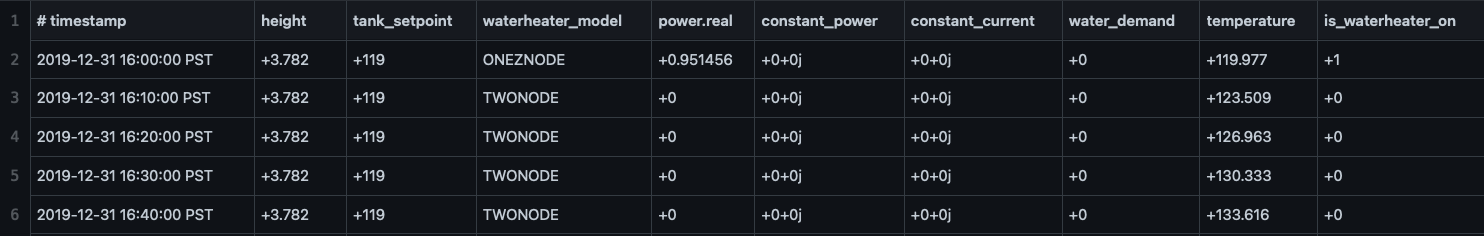
\includegraphics[width=1.1\columnwidth]{Pictures/HPWH_wrong_behavior.png}
        \caption{HPWH object in GLD does not respond to specified setpoints}
        \label{fig:HPWH}
    \end{figure}
    \begin{itemize}
        \item Comparing the HPWH behavior to the EWH, we can see the issue clearly. Figure \ref{fig:EWH} shows the EWH behavior under the same parameters.
    \end{itemize}
    \begin{figure}[htp!]
        \centering
        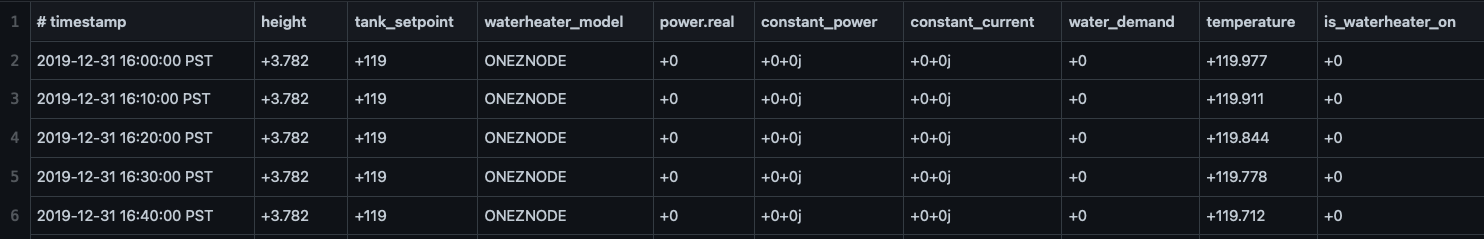
\includegraphics[width=1.1\columnwidth]{Pictures/EWH.png}
        \caption{EWH object in GLD responds properly to specified setpoints}
        \label{fig:EWH}
    \end{figure}
\newpage
    
\subsection{debugging}
\subsubsection{Related links}
\begin{itemize}
    \item Here's my conversation with Frank Tuffner, a GridLAB-D developer, regarding the HPWH. \href{https://sourceforge.net/p/gridlab-d/discussion/842562/thread/4a543d83a0/?limit=25#71e9}{Frank's input regarding HPWH issue.}
    \item On your computer, go to GLD folder $>$ residential $>$ open waterheater.cpp file.
\end{itemize}
\subsection{Water Heater Dynamic Driving Parameters}
\begin{itemize}
    \item Demand
    \begin{itemize}
        \item The higher the demand, the more quickly the thermocline drops.
    \end{itemize}
    \item Voltage
    \begin{itemize}
        \item The line voltage of the coil. The lower the voltage, the more slowly the thermocline rises.
    \end{itemize}
    \item Inlet water temperature
    \begin{itemize}
        \item The lower the inlet water temperature, the more heat needed to raise the temperature to the setpoint.
    \end{itemize}
    \item Indoor air temperature
    \begin{itemize}
        \item The higher the indoor temperature, the less heat loss through the jacket.
    \end{itemize}
\end{itemize}
\subsection{Heating Element Capacity}
The heating element capacity equation in the EWH is voltage dependant as shown in equation \ref{equ:HEC_EWH}.
\begin{equation}
    test = HeatingElementCapacity *(ActualVoltage)^2 / (NominalVoltage)^2
    \label{equ:HEC_EWH}
\end{equation}
However, the heating element capacity for the heat pump water heater does not have a voltage dependence as shown in equation \ref{equ:HEC_HPWH}.
\begin{equation}
    HeatingElementCapacity = (1.09 + (1.17 - 1.09) * (get_Tambient(location) -50) / (70 - 50)) * (0.379 + 0.00364 * Tw)
    \label{equ:HEC_HPWH}
\end{equation}

\subsection{Commented commands by GLD folks}
\begin{itemize}
    \item Heating element capacity (line 1634)
    \item Water temperature increment for onenode and twonode analysis (lines 1656 and 1684)
    \item Coesfficient of Performance (CoP) line 1731
\end{itemize}
\subsection{Water Heater Source Code Structure}
\begin{itemize}
    \item The code is defined by parameters instead of water heater models. 
    \item Some parameters, such as tank\textunderscore area, tank\textunderscore volume, tank\textunderscore height, etc are global as they work with all water heater models (i.e Electric, heat pump, and gas).
    \item Other parameters, such as heating element, need to be calculated when using Heat pump water heater model. The heating element in heat pump water heater is used as a backup.
\end{itemize}
\subsection{Errors Summary}
Running the HPWH object in GLD, we see the following errors:
\begin{itemize}
    \item The property is\textunderscore waterheater\textunderscore on is randomly 1 or 0. For a correct HPWH behavior, it should be 1 when there's sufficient water demand. Otherwise, it should always be zero.
    \item The waterheater\textunderscore model property should be ONEZNODE when there is no water demand. When there is water demand, there is inlet water pumped inside the tank. Therefore, both heating element capacity (top and bottom) should turn on. When both heating element capacity are on, the model switches to TWONODE model which is not the case in the HPWH. Refer to figure \ref{fig:EWH} and figure \ref{fig:HPWH} for a visual analysis.
\end{itemize}
\subsection{Questions}
\begin{itemize}
    \item I know the heating element is used as a backup in the HPWH. How is “backup” defined? Is it used where there’s a high water demand? How high should the water demand be to turn on the heating element?
    \begin{itemize}
        \item There are four modes in the A. O Smith units~\cite{r1}. These modes are listed as shown below:
        \begin{itemize}
            \item \textbf{Hybrid Mode:}
            \begin{itemize}
                \item This mode uses the dead-band algorithm. If the average tank temperature (the weighted temperature of the upper and lower thermostat) drops below 9F below the setpoint, then the HP turns on to heat the water.
                \item If the HP fails to heat the water to the setpoint (i.e due to high water demand.) and the average temperature drops more than 20F below the setpoint, then the upper heating element replaces the HP as the heating source. 
                \item The unit uses the HP until 75$\%$ of the available hot water has been depleted. 
            \end{itemize}
            \item \textbf{Efficiency Mode}
            \begin{itemize}
                \item This mode does not use the electric resistance elements, unless the ambient temperature is outside the safe operating range (45°–109°F) of the heat pump.
            \end{itemize}
            \item \textbf{EWH Mode}
            \begin{itemize}
                \item HPWH acts as EWH. Upper element turns ON first to heat the top of the tank and then lower element turns on to heat the bottom of the tank.
            \end{itemize}
            \item \textbf{Vacation Mode}
            \begin{itemize}
                \item Reduce the temperature setpoint (default is 60F)
            \end{itemize}
        \end{itemize}
    \end{itemize}
\end{itemize}
\subsubsection{Heating Element Operation Principle in HPWH}
The heating element operates under the following circumstances:
\begin{itemize}
    \item If the air temperature is outside the safe range (45 - 120F)
    \item If the water in the tank is significantly lower than the set point, the upper element operates. The difference between the tank temperature and the set point depends on the circumstances, but it is generally 25°–30°F.
    \item If the system senses that the water use is too high, the lower element operates. In general, 25–30 gal within a short time period is considered high water use. Once the lower electric resistance element engages, the entire tank is reheated like a traditional ERWH.
\end{itemize}
\newpage
\subsection{How does a Heat Pump Water-Heater work?}
    \begin{figure}[htp!]
        \centering
        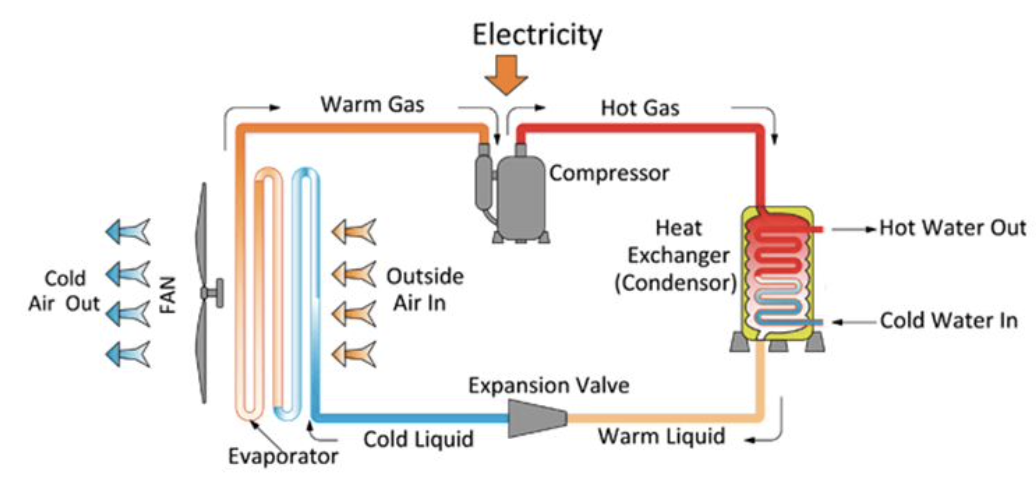
\includegraphics[width=1.1\columnwidth]{Pictures/HPWH_working_principle.png}
        \caption{source:\href{https://inukiengineering.com/heat-pump-water-heaters/}{nukiengineering.com}}
        \label{fig:EWH2}
    \end{figure}
I will start with a basic, however, very important thermodynamic principle. \textbf{HEAT ALWAYS GOES TO COLD.} Compressor increases the pressure of the gas passing through to make its temperature very high. This coil goes through the tank which heats up the water inside the tank (top portion). The heat of the gas gets released as it goes down the tank. The output of the tank is the same gas but with less hot temperature. The liquid goes through an expansion valve. The expansion valve "release" the liquid (less pressure therefore less heat) to make the liquid temperature less hot (cold). When the liquid goes through the evaporator, the temperature of the liquid is way less than the outside temperature. Therefore, the cold air gets dumped out and heat comes in. Thus, warm gas goes in to the compressor again and the same cycle is repeated.
\subsection{Coefficient of Performance (CoP)}
In EWH, we measure the efficiency to understand the performance of the WH. However, in the HPWH, we measure the CoP to see the ratio of useful heating or cooling provided to the required work as shown in equation \ref{equ:CoP}. \par
In GridLAB-D waterheater.cpp file, the CoP of the HPWH is defined with an equation that contains a set of integers. To make CoP more accessible, we need a more general equation. 
\begin{equation} \label{equ:CoP}
    CoP = \frac{E_{delivered}}{E_{in}}
\end{equation}
$E_{delivered}$ can be defined as:
\begin{equation}\label{equ:E_delivered}
    \Delta E_{delivered} = \frac{(V_{i}\rho_{w}C_{p,w}(T_{t,i}-T_{ref})) - (V_{i}\rho_{w}C_{p,w}(T_{t-1,i} - T_{ref}))}{t}
\end{equation}
Where:
\begin{itemize}
    \item $V_{i}$ = Volume of the node
    \item $\rho_{w}$ = water density of the node
    \item $C_{p,w}$ = water specific heat capacity.
    \item $T_{t,i}$ = Temperature of the node measured at time t.
    \item $T_{ref}$ = reference water temperature (default)
    \begin{itemize}
        \item For inlet water, the temperature is 60 $^{\circ}$.
    \end{itemize}
\end{itemize}
\newpage


\pagebreak
%----------------------------------------------------------------------------------------
%   Section: DCS and CTA-2045
%----------------------------------------------------------------------------------------
\newpage
\section{Summer 2021}
% \label{Summer2021}
All data and plots are in PSU Pwrlab Github account. If they're not there, contact midrar@pdx.edu
\pagebreak



%----------------------------------------------------------------------------------------
%   Section: Programmable Load Control
%----------------------------------------------------------------------------------------
\newpage
\section{Fall 2021}
% \label{Fall2021}
\subsection{Coefficient of Performance: V1}
The coefficient of performance is a measure of the useful energy transferred to the water in the tank per the system's supplied work. In other words, how much thermal energy can one get from 100 W input power, for example. The data obtained from this section are from EMCB use cases. There were different equations obtained from different resources~\cite{LeightonClarke,r1,Hudon}. All the aforementioned equations result in the following:
\begin{equation}\label{eq:cop}
    COP = \frac{Q}{E_{input}} = \frac{m \cdot C_{p} \cdot \Delta T}{E_{input}}
\end{equation}
Where:
\begin{itemize}
    \item m is the mass of the water in the tank in Pounds (lbm)
    \item $C_{p}$ is the specific heat of water ($\frac{Btu}{lbm \cdot \circ F}$)
    \item $\Delta T$ is the difference between the ambient temperature and the tank temperature in F.
    \item $E_{input}$ is the electrical power input in Watts. This includes the compressor and the heating element.
\end{itemize}

Equation~\ref{eq:cop} is applied to the morning shower in the EMCB studies. The morning shower is a 20 gallon water draw. The change in the water temperature during the heating process is linear. Therefore, a cumulative sum of the input power and then the average were calculated which resulted in 1680 W. Here's a list of the numerical value in equation \ref{eq:cop}:
\begin{itemize}
    \item $E_{input}$ = 1680 W.
    \item m = 50 gallon $\times$ 8.34 = 417 lbm.
    \item C$_{p}$ = 1.001 $\frac{Btu}{lbm \cdot ^{\circ}F}$.
    \item $T_{ambient}$ = 75 $^{\circ}$F
\end{itemize}

For example, if the current temperature in the tank is 100 $^{\circ}F$, then the COP can be calculated as follows:

\begin{equation}
    COP = \frac{(417 [lbm] \times 1.001 \frac{Btu}{lbm \cdot F} \times (100 - 75) [F]) \times 0.293 }{1680 [W]}
    \&=1.82
\end{equation}

\begin{figure}[htp!]
    \centering
    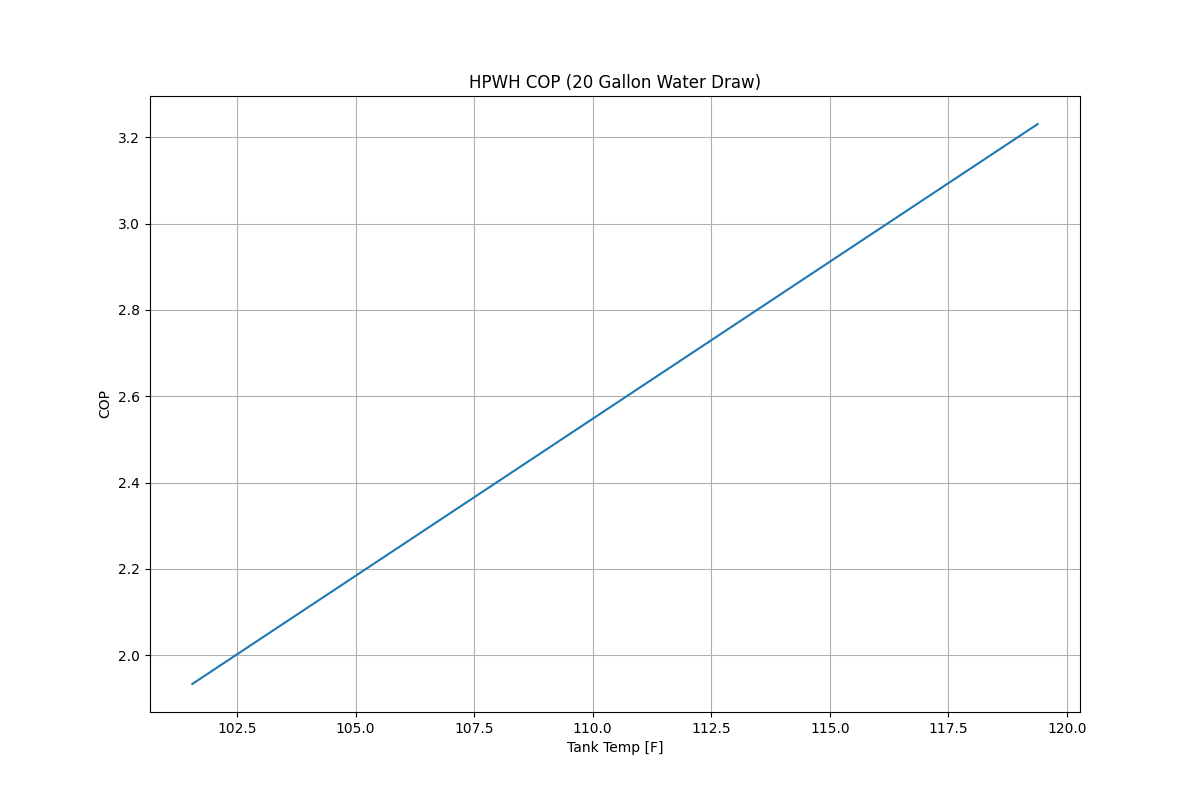
\includegraphics[width=0.9\columnwidth]{Pictures/cop_sim.png}
    \caption{\gls{hpwh} COP: 20 Gallon Water Draw}
    \label{fig:cop}
\end{figure}
\newpage
\subsection{Coefficient of Performance: V2}
The equation used to calculate and plot the COP of the \gls{hpwh} is as follows:

\begin{equation}
    COP = \frac{EnergyTake}{Watts}
\end{equation}

The \gls{hpwh} was set to vacation mode for three days. After, the \gls{hpwh} was switched to Hybrid mode. Here's the data when the \gls{hpwh} switch ON.


\begin{longtable}{|l|l|l|}\label{table:hpwh_vacation_hybrid}

time & EnergyTake & Watts  \\ \hline

Mon Sep 20 12:17:12 2021 &               2775 &       4449.0300 \\ \hline
Mon Sep 20 12:18:12 2021 &               2775 &       4665.8100 \\ \hline
Mon Sep 20 12:19:13 2021 &               2625 &       4686.4500 \\ \hline
Mon Sep 20 12:20:14 2021 &               2550 &       4717.4200 \\ \hline
Mon Sep 20 12:21:14 2021 &               2250 &       4738.0600 \\ \hline
Mon Sep 20 12:22:15 2021 &               2175 &       4748.3900 \\ \hline
Mon Sep 20 12:23:15 2021 &               2025 &       4707.1000 \\ \hline
Mon Sep 20 12:24:16 2021 &               2025 &       4769.0300 \\ \hline
Mon Sep 20 12:25:17 2021 &               1875 &       4769.0300 \\ \hline
Mon Sep 20 12:26:17 2021 &               1800 &       4758.7100 \\ \hline
Mon Sep 20 12:27:18 2021 &               1725 &       4769.0300 \\ \hline
Mon Sep 20 12:28:18 2021 &               1725 &       4769.0300 \\ \hline
Mon Sep 20 12:29:19 2021 &               1650 &       4779.3500 \\ \hline
Mon Sep 20 12:30:19 2021 &               1575 &       4676.1300 \\ \hline
Mon Sep 20 12:31:20 2021 &               1575 &       4707.1000 \\ \hline
Mon Sep 20 12:32:21 2021 &               1425 &       4645.1600 \\ \hline
Mon Sep 20 12:33:21 2021 &               1425 &       4696.7700 \\ \hline
Mon Sep 20 12:34:22 2021 &               1275 &       4696.7700 \\ \hline
Mon Sep 20 12:35:22 2021 &               1200 &       4686.4500 \\ \hline
Mon Sep 20 12:36:23 2021 &               1050 &        392.2580 \\ \hline
Mon Sep 20 12:37:24 2021 &               1050 &        402.5810 \\ \hline
Mon Sep 20 12:38:24 2021 &               1050 &        402.5810 \\ \hline
Mon Sep 20 12:39:25 2021 &                975 &        402.5810 \\ \hline
Mon Sep 20 12:40:25 2021 &                975 &        402.5810 \\ \hline
Mon Sep 20 12:41:26 2021 &                975 &        402.5810 \\ \hline
Mon Sep 20 12:42:27 2021 &                975 &        402.5810 \\ \hline
Mon Sep 20 12:43:27 2021 &                975 &        402.5810 \\ \hline
Mon Sep 20 12:44:28 2021 &                975 &        402.5810 \\ \hline
Mon Sep 20 12:45:28 2021 &                975 &        402.5810 \\ \hline
Mon Sep 20 12:46:29 2021 &                975 &        412.9030 \\ \hline
Mon Sep 20 12:47:29 2021 &                975 &        402.5810 \\ \hline
Mon Sep 20 12:48:30 2021 &                975 &        402.5810 \\ \hline
Mon Sep 20 12:49:31 2021 &                975 &        402.5810 \\ \hline
Mon Sep 20 12:50:31 2021 &                900 &        402.5810 \\ \hline
Mon Sep 20 12:51:32 2021 &                900 &        412.9030 \\ \hline
Mon Sep 20 12:52:32 2021 &                825 &        412.9030 \\ \hline
Mon Sep 20 12:53:33 2021 &                825 &        402.5810 \\ \hline
Mon Sep 20 12:54:34 2021 &                825 &        412.9030 \\ \hline
Mon Sep 20 12:55:34 2021 &                825 &        412.9030 \\ \hline
Mon Sep 20 12:56:35 2021 &                825 &        412.9030 \\ \hline
Mon Sep 20 12:57:35 2021 &                825 &        412.9030 \\ \hline
Mon Sep 20 12:58:36 2021 &                825 &        412.9030 \\ \hline
Mon Sep 20 12:59:36 2021 &                825 &        412.9030 \\ \hline
Mon Sep 20 13:00:37 2021 &                750 &        412.9030 \\ \hline
Mon Sep 20 13:01:38 2021 &                750 &        412.9030 \\ \hline
Mon Sep 20 13:02:38 2021 &                750 &        412.9030 \\ \hline
Mon Sep 20 13:03:39 2021 &                750 &        412.9030 \\ \hline
Mon Sep 20 13:04:39 2021 &                600 &        412.9030 \\ \hline
Mon Sep 20 13:05:40 2021 &                600 &        423.2260 \\ \hline
Mon Sep 20 13:06:41 2021 &                600 &        423.2260 \\ \hline
Mon Sep 20 13:07:41 2021 &                600 &        423.2260 \\ \hline
Mon Sep 20 13:08:42 2021 &                600 &        423.2260 \\ \hline
Mon Sep 20 13:09:42 2021 &                600 &        423.2260 \\ \hline
Mon Sep 20 13:10:43 2021 &                600 &        423.2260 \\ \hline
Mon Sep 20 13:11:43 2021 &                600 &        423.2260 \\ \hline
Mon Sep 20 13:12:44 2021 &                600 &        423.2260 \\ \hline
Mon Sep 20 13:13:45 2021 &                600 &        423.2260 \\ \hline
Mon Sep 20 13:14:45 2021 &                525 &        423.2260 \\ \hline
Mon Sep 20 13:15:46 2021 &                525 &        423.2260 \\ \hline
Mon Sep 20 13:16:46 2021 &                525 &        423.2260 \\ \hline
Mon Sep 20 13:17:47 2021 &                525 &        423.2260 \\ \hline
Mon Sep 20 13:18:48 2021 &                525 &        433.5480 \\ \hline
Mon Sep 20 13:19:48 2021 &                525 &        433.5480 \\ \hline
Mon Sep 20 13:20:49 2021 &                525 &        433.5480 \\ \hline
Mon Sep 20 13:21:49 2021 &                525 &        433.5480 \\ \hline
Mon Sep 20 13:22:50 2021 &                450 &        433.5480 \\ \hline
Mon Sep 20 13:23:51 2021 &                450 &        433.5480 \\ \hline
Mon Sep 20 13:24:51 2021 &                375 &        433.5480 \\ \hline
Mon Sep 20 13:25:52 2021 &                375 &        433.5480 \\ \hline
Mon Sep 20 13:26:52 2021 &                375 &        433.5480 \\ \hline
Mon Sep 20 13:27:53 2021 &                375 &        433.5480 \\ \hline
Mon Sep 20 13:28:53 2021 &                375 &        433.5480 \\ \hline
Mon Sep 20 13:29:54 2021 &                225 &        433.5480 \\ \hline
Mon Sep 20 13:30:55 2021 &                225 &        433.5480 \\ \hline
Mon Sep 20 13:31:55 2021 &                225 &        433.5480 \\ \hline
Mon Sep 20 13:32:56 2021 &                225 &        433.5480 \\ \hline
Mon Sep 20 13:33:56 2021 &                225 &        433.5480 \\ \hline
Mon Sep 20 13:34:57 2021 &                225 &        433.5480 \\ \hline
Mon Sep 20 13:35:58 2021 &                225 &        443.8710 \\ \hline
Mon Sep 20 13:36:58 2021 &                225 &        443.8710 \\ \hline
Mon Sep 20 13:37:59 2021 &                225 &        443.8710 \\ \hline
Mon Sep 20 13:38:59 2021 &                 75 &        443.8710 \\ \hline
Mon Sep 20 13:40:00 2021 &                 75 &        443.8710 \\ \hline
Mon Sep 20 13:41:01 2021 &                 75 &        433.5480 \\ \hline
Mon Sep 20 13:42:01 2021 &                 75 &        433.5480 \\ \hline
Mon Sep 20 13:43:02 2021 &                 75 &        433.5480 \\ \hline
Mon Sep 20 13:44:02 2021 &                 75 &        443.8710 \\ \hline
Mon Sep 20 13:45:03 2021 &                 75 &        443.8710 \\ \hline
Mon Sep 20 13:46:03 2021 &                  0 &        443.8710 \\ \hline
Mon Sep 20 13:47:04 2021 &                  0 &        443.8710 \\ \hline
Mon Sep 20 13:48:05 2021 &                  0 &        443.8710 \\ \hline
Mon Sep 20 13:49:05 2021 &                  0 &        454.1940 \\ \hline
Mon Sep 20 13:50:06 2021 &                  0 &        443.8710 \\ \hline
Mon Sep 20 13:51:06 2021 &                  0 &        454.1940 \\ \hline
Mon Sep 20 13:52:07 2021 &                  0 &        454.1940 \\ \hline
Mon Sep 20 13:53:07 2021 &                  0 &        454.1940 \\ \hline
Mon Sep 20 13:54:08 2021 &                  0 &        443.8710 \\ \hline
Mon Sep 20 13:55:08 2021 &                  0 &        454.1940 \\ \hline
Mon Sep 20 13:56:09 2021 &                  0 &        454.1940 \\ \hline
Mon Sep 20 13:57:09 2021 &                  0 &        454.1940 \\ \hline
Mon Sep 20 13:58:10 2021 &                  0 &        454.1940 \\ \hline
Mon Sep 20 13:59:11 2021 &                  0 &        454.1940 \\ \hline
Mon Sep 20 14:00:11 2021 &                  0 &        454.1940 \\ \hline
Mon Sep 20 14:01:12 2021 &                  0 &        454.1940 \\ \hline
Mon Sep 20 14:02:12 2021 &                  0 &        454.1940 \\ \hline
Mon Sep 20 14:03:13 2021 &                  0 &        454.1940 \\ \hline
Mon Sep 20 14:04:13 2021 &                  0 &        454.1940 \\ \hline
Mon Sep 20 14:05:14 2021 &                  0 &        464.5160 \\ \hline
Mon Sep 20 14:06:15 2021 &                  0 &        454.1940 \\ \hline
Mon Sep 20 14:07:15 2021 &                  0 &        454.1940 \\ \hline
Mon Sep 20 14:08:16 2021 &                  0 &        454.1940 \\ \hline
Mon Sep 20 14:09:16 2021 &                  0 &        454.1940 \\ \hline
Mon Sep 20 14:10:17 2021 &                  0 &        454.1940 \\ \hline
Mon Sep 20 14:11:17 2021 &                  0 &         41.2903 \\ \hline
Mon Sep 20 14:12:18 2021 &                  0 &         30.9677 \\ \hline
Mon Sep 20 14:13:19 2021 &                  0 &         41.2903 \\ \hline
Mon Sep 20 14:14:19 2021 &                  0 &         41.2903 \\ \hline
Mon Sep 20 15:20:57 2021 &                  0 &         10.3226 \\ \hline
\end{longtable}

The \gls{hpwh} was ON for 81 minutes to heat the water up to the setpoints, 120 $^{\circ}F$. Therefore, the values of watts consumed was converted to Watts-hour as follows:
\begin{equation}
    Wh = Watts \times \frac{x-1}{60}
\end{equation}
Where x is the duration of the heating process.

The following figures show the COP VS:
\begin{itemize}
    \item time
    \item EnergyTake
    \item Line fit
\end{itemize}
\textbf{The average COP is 3.2}

\begin{figure}[htp!]
    \centering
    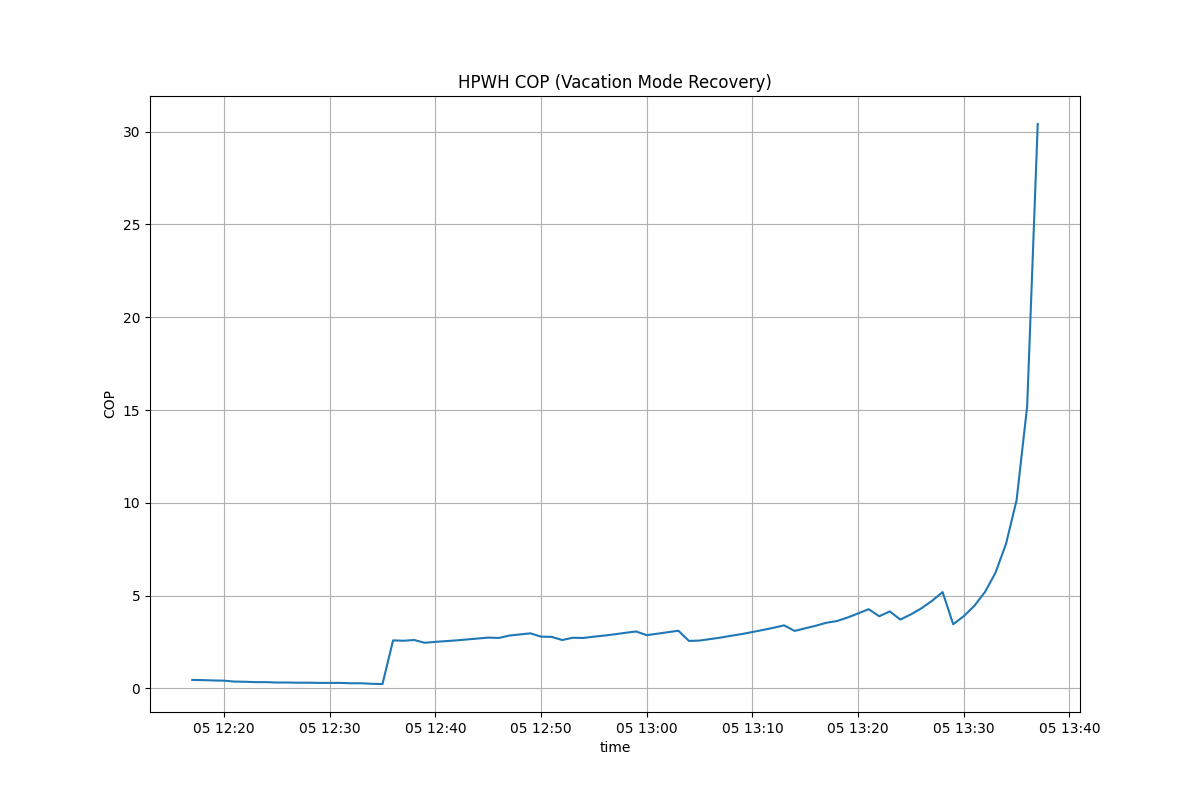
\includegraphics[width=0.9\columnwidth]{Pictures/cop_vs_time.png}
    \caption{\gls{hpwh} COP vs Time: Vacation Mode Recovery}
    \label{fig:copvstime}
\end{figure}

\begin{figure}[htp!]
    \centering
    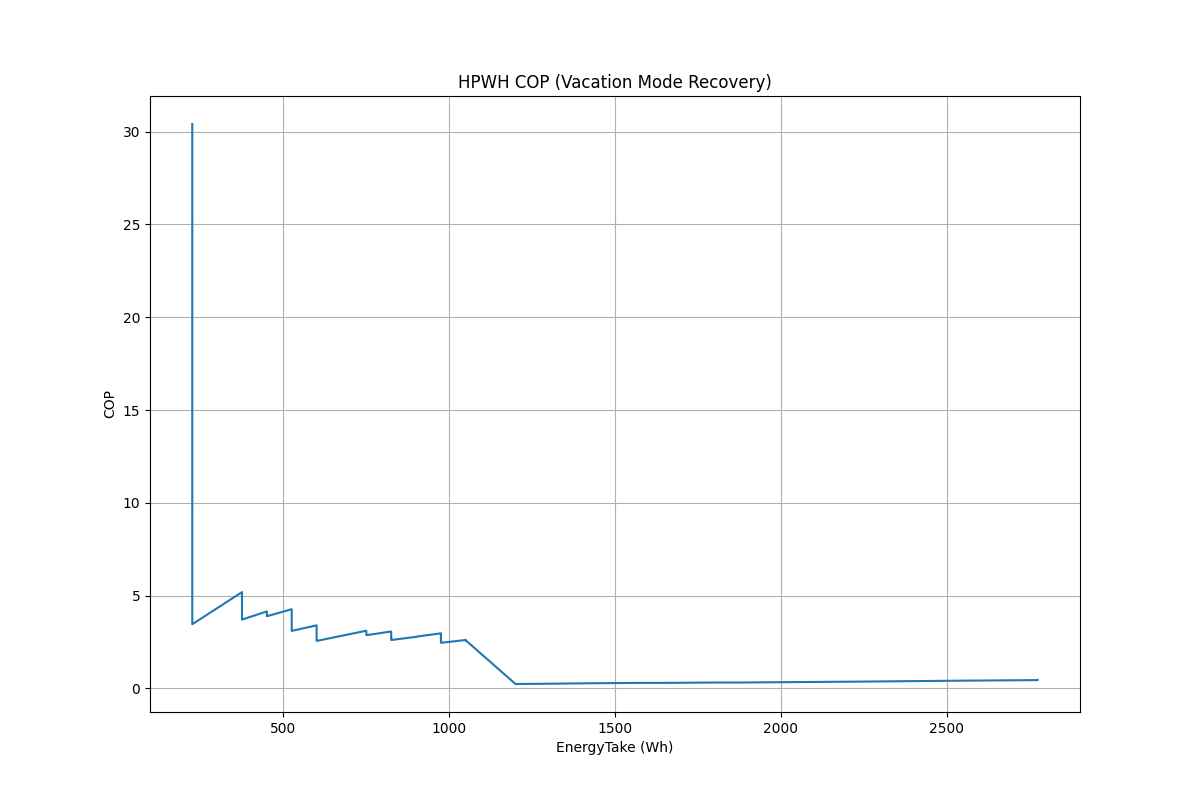
\includegraphics[width=0.9\columnwidth]{Pictures/cop_vs_EnergyTake.png}
    \caption{\gls{hpwh} COP vs EnergyTake: Vacation Mode Recovery}
    \label{fig:copvsenergytake}
\end{figure}
\newpage

\subsection{October 12}
In order to proceed with the COP calculations, we need to calculate the watts and watts-hour used by the water heater every time step. The following sections will walk through the process in steps.
\subsubsection{Testing}

In order to measure the output energy of the water heater, we need to the compressor to run as long as possible. Therefore, the efficiency mode was used. The hot water inside the tank was completely drawn by opening the valve and let the water flow. After that the unit was set in vacation mode for a few days (extra precautions. The unit should be good to go from opening the valve). Then the unit was turned on in efficieny mode. The efficiency mode allows the compressor to do most of the work to heat the water instead of the heating element. The data collected from this testing is shown below:


\begin{longtable}{|l|r|r|}\label{tab:data_v-e HPWH}

               timestamp &  real\_available\_Wh &  consumed\_watts \\ 
\hline
\endfirsthead

               timestamp &  real\_available\_Wh &  consumed\_watts

\endhead

\multicolumn{3}{r}{{Continued on next page}} \\

\endfoot

\endlastfoot
Fri Oct  8 12:26:59 2021 &               4050 &       4459.3500 \\ \hline
Fri Oct  8 12:28:00 2021 &               4050 &       4676.1300 \\ \hline
Fri Oct  8 12:29:01 2021 &               3750 &       4665.8100 \\ \hline
Fri Oct  8 12:30:01 2021 &               3525 &       4727.7400 \\ \hline
Fri Oct  8 12:31:02 2021 &               3450 &       4696.7700 \\ \hline
Fri Oct  8 12:32:03 2021 &               3375 &       4707.1000 \\ \hline
Fri Oct  8 12:33:04 2021 &               3225 &       4707.1000 \\ \hline
Fri Oct  8 12:34:05 2021 &               3225 &       4696.7700 \\ \hline
Fri Oct  8 12:35:05 2021 &               3000 &       4717.4200 \\ \hline
Fri Oct  8 12:36:06 2021 &               3000 &       4696.7700 \\ \hline
Fri Oct  8 12:37:07 2021 &               2925 &       4707.1000 \\ \hline
Fri Oct  8 12:38:08 2021 &               2775 &       4727.7400 \\ \hline
Fri Oct  8 12:39:09 2021 &               2700 &       4748.3900 \\ \hline
Fri Oct  8 12:40:09 2021 &               2700 &       4696.7700 \\ \hline
Fri Oct  8 12:41:10 2021 &               2625 &       4748.3900 \\ \hline
Fri Oct  8 12:42:11 2021 &               2550 &       4696.7700 \\ \hline
Fri Oct  8 12:43:12 2021 &               2550 &       4717.4200 \\ \hline
Fri Oct  8 12:44:13 2021 &               2475 &       4738.0600 \\ \hline
Fri Oct  8 12:45:13 2021 &               2400 &       4748.3900 \\ \hline
Fri Oct  8 12:46:14 2021 &               2325 &       4696.7700 \\ \hline
Fri Oct  8 12:47:15 2021 &               2250 &       4717.4200 \\ \hline
Fri Oct  8 12:48:16 2021 &               2175 &       4707.1000 \\ \hline
Fri Oct  8 12:49:17 2021 &               2100 &        350.9680 \\ \hline
Fri Oct  8 12:50:17 2021 &               2100 &        350.9680 \\ \hline
Fri Oct  8 12:51:18 2021 &               2025 &        350.9680 \\ \hline
Fri Oct  8 12:52:19 2021 &               2025 &        350.9680 \\ \hline
Fri Oct  8 12:53:20 2021 &               1950 &        350.9680 \\ \hline
Fri Oct  8 12:54:20 2021 &               1950 &        361.2900 \\ \hline
Fri Oct  8 12:55:21 2021 &               1950 &        350.9680 \\ \hline
Fri Oct  8 12:56:22 2021 &               2025 &        350.9680 \\ \hline
Fri Oct  8 12:57:23 2021 &               2025 &        350.9680 \\ \hline
Fri Oct  8 12:58:24 2021 &               2025 &        361.2900 \\ \hline
Fri Oct  8 12:59:24 2021 &               2025 &        350.9680 \\ \hline
Fri Oct  8 13:00:25 2021 &               2025 &        361.2900 \\ \hline
Fri Oct  8 13:01:26 2021 &               2025 &        361.2900 \\ \hline
Fri Oct  8 13:02:27 2021 &               2025 &        361.2900 \\ \hline
Fri Oct  8 13:03:28 2021 &               1950 &        361.2900 \\ \hline
Fri Oct  8 13:04:28 2021 &               1950 &        361.2900 \\ \hline
Fri Oct  8 13:05:29 2021 &               1950 &        361.2900 \\ \hline
Fri Oct  8 13:06:30 2021 &               1950 &        361.2900 \\ \hline
Fri Oct  8 13:07:31 2021 &               1800 &        361.2900 \\ \hline
Fri Oct  8 13:08:32 2021 &               1800 &        361.2900 \\ \hline
Fri Oct  8 13:09:32 2021 &               1725 &        371.6130 \\ \hline
Fri Oct  8 13:10:33 2021 &               1725 &        361.2900 \\ \hline
Fri Oct  8 13:11:34 2021 &               1725 &        361.2900 \\ \hline
Fri Oct  8 13:12:35 2021 &               1725 &        371.6130 \\ \hline
Fri Oct  8 13:13:36 2021 &               1650 &        371.6130 \\ \hline
Fri Oct  8 13:14:36 2021 &               1650 &        371.6130 \\ \hline
Fri Oct  8 13:15:37 2021 &               1650 &        371.6130 \\ \hline
Fri Oct  8 13:16:38 2021 &               1650 &        371.6130 \\ \hline
Fri Oct  8 13:17:39 2021 &               1650 &        371.6130 \\ \hline
Fri Oct  8 13:18:40 2021 &               1575 &        371.6130 \\ \hline
Fri Oct  8 13:19:40 2021 &               1575 &        371.6130 \\ \hline
Fri Oct  8 13:20:41 2021 &               1575 &        381.9350 \\ \hline
Fri Oct  8 13:21:42 2021 &               1575 &        371.6130 \\ \hline
Fri Oct  8 13:22:43 2021 &               1575 &        381.9350 \\ \hline
Fri Oct  8 13:23:44 2021 &               1575 &        381.9350 \\ \hline
Fri Oct  8 13:24:44 2021 &               1575 &        381.9350 \\ \hline
Fri Oct  8 13:25:45 2021 &               1425 &        381.9350 \\ \hline
Fri Oct  8 13:26:46 2021 &               1425 &        381.9350 \\ \hline
Fri Oct  8 13:27:47 2021 &               1425 &        381.9350 \\ \hline
Fri Oct  8 13:28:48 2021 &               1425 &        381.9350 \\ \hline
Fri Oct  8 13:29:48 2021 &               1425 &        381.9350 \\ \hline
Fri Oct  8 13:30:49 2021 &               1425 &        381.9350 \\ \hline
Fri Oct  8 13:31:50 2021 &               1350 &        381.9350 \\ \hline
Fri Oct  8 13:32:51 2021 &               1350 &        381.9350 \\ \hline
Fri Oct  8 13:33:52 2021 &               1275 &        381.9350 \\ \hline
Fri Oct  8 13:34:52 2021 &               1275 &        392.2580 \\ \hline
Fri Oct  8 13:35:53 2021 &               1275 &        392.2580 \\ \hline
Fri Oct  8 13:36:54 2021 &               1275 &        381.9350 \\ \hline
Fri Oct  8 13:37:55 2021 &               1275 &        381.9350 \\ \hline
Fri Oct  8 13:38:56 2021 &               1275 &        392.2580 \\ \hline
Fri Oct  8 13:39:56 2021 &               1275 &        392.2580 \\ \hline
Fri Oct  8 13:40:57 2021 &               1200 &        392.2580 \\ \hline
Fri Oct  8 13:41:58 2021 &               1200 &        392.2580 \\ \hline
Fri Oct  8 13:42:59 2021 &               1200 &        392.2580 \\ \hline
Fri Oct  8 13:43:59 2021 &               1050 &        392.2580 \\ \hline
Fri Oct  8 13:45:00 2021 &               1050 &        402.5810 \\ \hline
Fri Oct  8 13:46:01 2021 &               1050 &        392.2580 \\ \hline
Fri Oct  8 13:47:02 2021 &               1050 &        392.2580 \\ \hline
Fri Oct  8 13:48:03 2021 &               1050 &        402.5810 \\ \hline
Fri Oct  8 13:49:03 2021 &               1050 &        402.5810 \\ \hline
Fri Oct  8 13:50:04 2021 &               1050 &        402.5810 \\ \hline
Fri Oct  8 13:51:05 2021 &               1050 &        402.5810 \\ \hline
Fri Oct  8 13:52:06 2021 &                975 &        402.5810 \\ \hline
Fri Oct  8 13:53:07 2021 &                975 &        402.5810 \\ \hline
Fri Oct  8 13:54:07 2021 &                975 &        402.5810 \\ \hline
Fri Oct  8 13:55:08 2021 &                975 &        402.5810 \\ \hline
Fri Oct  8 13:56:09 2021 &                975 &        402.5810 \\ \hline
Fri Oct  8 13:57:10 2021 &                975 &        402.5810 \\ \hline
Fri Oct  8 13:58:11 2021 &                975 &        402.5810 \\ \hline
Fri Oct  8 13:59:11 2021 &                900 &        402.5810 \\ \hline
Fri Oct  8 14:00:12 2021 &                900 &        402.5810 \\ \hline
Fri Oct  8 14:01:13 2021 &                825 &        402.5810 \\ \hline
Fri Oct  8 14:02:14 2021 &                825 &        412.9030 \\ \hline
Fri Oct  8 14:03:15 2021 &                825 &        412.9030 \\ \hline
Fri Oct  8 14:04:15 2021 &                825 &        412.9030 \\ \hline
Fri Oct  8 14:05:16 2021 &                825 &        412.9030 \\ \hline
Fri Oct  8 14:06:17 2021 &                825 &        412.9030 \\ \hline
Fri Oct  8 14:07:18 2021 &                825 &        412.9030 \\ \hline
Fri Oct  8 14:08:19 2021 &                750 &        412.9030 \\ \hline
Fri Oct  8 14:09:19 2021 &                750 &        412.9030 \\ \hline
Fri Oct  8 14:10:20 2021 &                750 &        412.9030 \\ \hline
Fri Oct  8 14:11:21 2021 &                750 &        412.9030 \\ \hline
Fri Oct  8 14:12:22 2021 &                600 &        423.2260 \\ \hline
Fri Oct  8 14:13:23 2021 &                600 &        412.9030 \\ \hline
Fri Oct  8 14:14:23 2021 &                600 &        423.2260 \\ \hline
Fri Oct  8 14:15:24 2021 &                600 &        423.2260 \\ \hline
Fri Oct  8 14:16:25 2021 &                600 &        412.9030 \\ \hline
Fri Oct  8 14:17:26 2021 &                600 &        423.2260 \\ \hline
Fri Oct  8 14:18:27 2021 &                600 &        412.9030 \\ \hline
Fri Oct  8 14:19:27 2021 &                600 &        423.2260 \\ \hline
Fri Oct  8 14:20:28 2021 &                600 &        423.2260 \\ \hline
Fri Oct  8 14:21:29 2021 &                525 &        423.2260 \\ \hline
Fri Oct  8 14:22:30 2021 &                525 &        423.2260 \\ \hline
Fri Oct  8 14:23:31 2021 &                525 &        423.2260 \\ \hline
Fri Oct  8 14:24:31 2021 &                525 &        433.5480 \\ \hline
Fri Oct  8 14:25:32 2021 &                525 &        423.2260 \\ \hline
Fri Oct  8 14:26:33 2021 &                525 &        423.2260 \\ \hline
Fri Oct  8 14:27:34 2021 &                525 &        423.2260 \\ \hline
Fri Oct  8 14:28:35 2021 &                450 &        433.5480 \\ \hline
Fri Oct  8 14:29:35 2021 &                450 &        433.5480 \\ \hline
Fri Oct  8 14:30:36 2021 &                375 &        433.5480 \\ \hline
Fri Oct  8 14:31:37 2021 &                375 &        433.5480 \\ \hline
Fri Oct  8 14:32:38 2021 &                375 &        433.5480 \\ \hline
Fri Oct  8 14:33:39 2021 &                375 &        433.5480 \\ \hline
Fri Oct  8 14:34:39 2021 &                375 &        433.5480 \\ \hline
Fri Oct  8 14:35:40 2021 &                225 &        433.5480 \\ \hline
Fri Oct  8 14:36:41 2021 &                225 &        433.5480 \\ \hline
Fri Oct  8 14:37:42 2021 &                225 &        433.5480 \\ \hline
Fri Oct  8 14:38:43 2021 &                225 &        433.5480 \\ \hline
Fri Oct  8 14:39:43 2021 &                225 &        443.8710 \\ \hline
Fri Oct  8 14:40:44 2021 &                225 &        443.8710 \\ \hline
Fri Oct  8 14:41:45 2021 &                225 &        443.8710 \\ \hline
Fri Oct  8 14:42:46 2021 &                 75 &        443.8710 \\ \hline
Fri Oct  8 14:43:47 2021 &                 75 &        443.8710 \\ \hline
Fri Oct  8 14:44:47 2021 &                 75 &        443.8710 \\ \hline
Fri Oct  8 14:45:48 2021 &                 75 &        443.8710 \\ \hline
Fri Oct  8 14:46:49 2021 &                 75 &        443.8710 \\ \hline
Fri Oct  8 14:47:50 2021 &                 75 &        443.8710 \\ \hline
Fri Oct  8 14:48:50 2021 &                 75 &        443.8710 \\ \hline
Fri Oct  8 14:49:51 2021 &                  0 &        443.8710 \\ \hline
Fri Oct  8 14:50:52 2021 &                  0 &        443.8710 \\ \hline
Fri Oct  8 14:51:53 2021 &                  0 &        443.8710 \\ \hline
Fri Oct  8 14:52:54 2021 &                  0 &        454.1940 \\ \hline
Fri Oct  8 14:53:54 2021 &                  0 &        443.8710 \\ \hline
Fri Oct  8 14:54:55 2021 &                  0 &        443.8710 \\ \hline
Fri Oct  8 14:55:56 2021 &                  0 &        454.1940 \\ \hline
Fri Oct  8 14:56:57 2021 &                  0 &        443.8710 \\ \hline
Fri Oct  8 14:57:58 2021 &                  0 &        443.8710 \\ \hline
Fri Oct  8 14:58:58 2021 &                  0 &        454.1940 \\ \hline
Fri Oct  8 14:59:59 2021 &                  0 &        454.1940 \\ \hline
Fri Oct  8 15:01:00 2021 &                  0 &        454.1940 \\ \hline
Fri Oct  8 15:02:01 2021 &                  0 &        454.1940 \\ \hline
Fri Oct  8 15:03:02 2021 &                  0 &        454.1940 \\ \hline
Fri Oct  8 15:04:02 2021 &                  0 &        454.1940 \\ \hline
Fri Oct  8 15:05:03 2021 &                  0 &        454.1940 \\ \hline
Fri Oct  8 15:06:04 2021 &                  0 &        454.1940 \\ \hline
Fri Oct  8 15:07:05 2021 &                  0 &        464.5160 \\ \hline
Fri Oct  8 15:08:06 2021 &                  0 &        454.1940 \\ \hline
Fri Oct  8 15:09:06 2021 &                  0 &        454.1940 \\ \hline
Fri Oct  8 15:10:07 2021 &                  0 &        454.1940 \\ \hline
Fri Oct  8 15:11:08 2021 &                  0 &        454.1940 \\ \hline
Fri Oct  8 15:12:09 2021 &                  0 &        464.5160 \\ \hline
Fri Oct  8 15:13:10 2021 &                  0 &        464.5160 \\ \hline
Fri Oct  8 15:14:10 2021 &                  0 &         41.2903 \\ \hline
Fri Oct  8 15:15:11 2021 &                  0 &         30.9677 \\ \hline
Fri Oct  8 15:16:12 2021 &                  0 &         41.2903 \\ \hline
Fri Oct  8 15:17:13 2021 &                  0 &         41.2903 \\ \hline

\end{longtable}


\subsubsection{EnergyTake and Watts}

The COP equation that I've been using so far is the following:

\begin{equation}
    COP = \frac{EnergyTake}{Watts}
\end{equation}

The EnergyTake definition, from $CTA-2045$ as shown in figure~\ref{fig:cta_def}, is the current available energy in the tank. It does not represent the output energy with every timestep. However, the output energy can be represented by the difference between each ET value in each timestep, which in this case, would be 75 Wh. Table~\ref{tab:data_v-e HPWH} shows the data collected from the \gls{hpwh} durint the testing. The watts conversion to Watts-hour is the same way used as before. No changes. 

\begin{figure}[htp!]
    \centering
    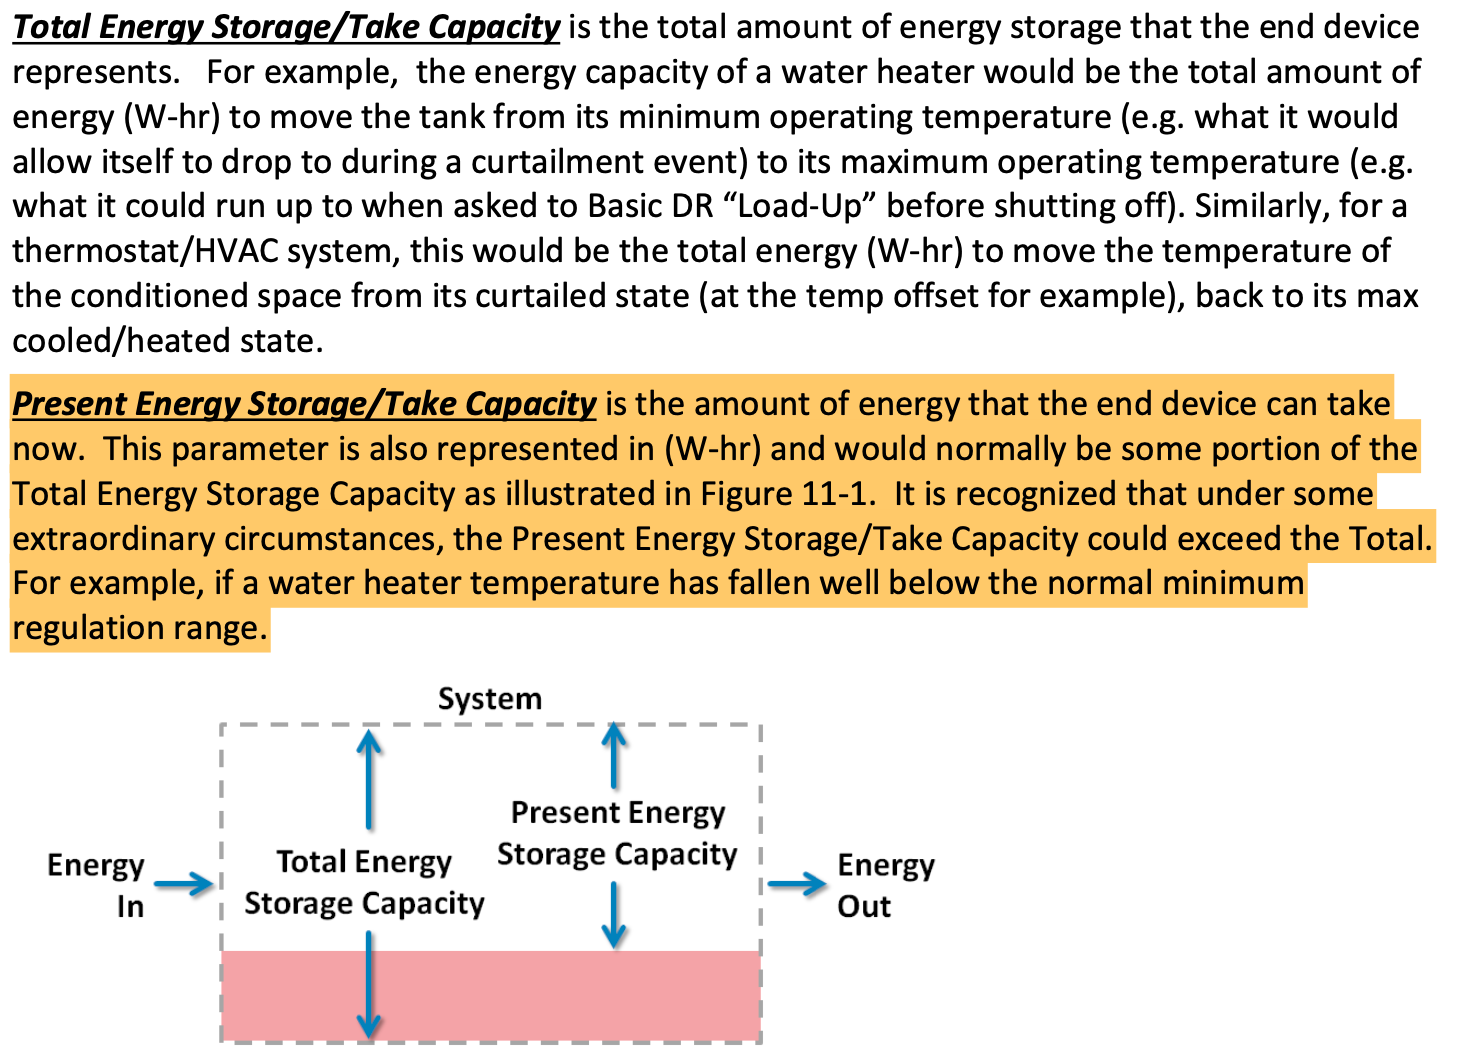
\includegraphics[width=0.9\columnwidth]{Pictures/cta_def.png}
    \caption{CTA-2045 EnergyTake Definition}
    \label{fig:cta_def}
\end{figure}

\subsubsection{Data Used for Calculations}
\begin{table}[ht!]
\caption{\gls{hpwh} Data Used For Calculating COP in this Section}
\begin{adjustbox}{max width=\textwidth}
\begin{tabular}{|l|r|r|r|r|r|r|}
\hline
    time &  EnergyTake (Wh) &  consumed\_watts (Watts) &  time\_diff &  average\_watts &  Energy in &   cop \\ \hline

12:49:17 &               2100 &         350.968 &       1.02 &         350.97 &   5.97 & 12.56 \\ \hline
12:51:18 &               2025 &         350.968 &       2.02 &         350.97 &  11.82 &  6.35 \\ \hline
12:53:20 &               1950 &         350.968 &       2.03 &         350.97 &  11.87 &  6.32 \\ \hline
13:07:31 &               1800 &         361.290 &      14.18 &         361.29 &  85.38 &  0.88 \\ \hline
13:09:32 &               1725 &         371.613 &       2.02 &         371.61 &  12.51 &  6.00 \\ \hline
13:13:36 &               1650 &         371.613 &       4.07 &         371.61 &  25.21 &  2.98 \\ \hline
13:18:40 &               1575 &         371.613 &       5.07 &         371.61 &  31.40 &  2.39 \\ \hline
13:25:45 &               1425 &         381.935 &       7.08 &         381.94 &  45.07 &  1.66 \\ \hline
13:31:50 &               1350 &         381.935 &       6.08 &         381.94 &  38.70 &  1.94 \\ \hline
13:33:52 &               1275 &         381.935 &       2.03 &         381.94 &  12.92 &  5.80 \\ \hline
13:40:57 &               1200 &         392.258 &       7.08 &         392.26 &  46.29 &  1.62 \\ \hline
13:43:59 &               1050 &         392.258 &       3.03 &         392.26 &  19.81 &  3.79 \\ \hline
13:52:06 &                975 &         402.581 &       8.12 &         402.58 &  54.48 &  1.38 \\ \hline
13:59:11 &                900 &         402.581 &       7.08 &         402.58 &  47.50 &  1.58 \\ \hline
14:01:13 &                825 &         402.581 &       2.03 &         402.58 &  13.62 &  5.51 \\ \hline
14:08:19 &                750 &         412.903 &       7.10 &         412.90 &  48.86 &  1.53 \\ \hline
14:12:22 &                600 &         423.226 &       4.05 &         423.23 &  28.57 &  2.63 \\ \hline
14:21:29 &                525 &         423.226 &       9.12 &         423.23 &  64.33 &  1.17 \\ \hline
14:28:35 &                450 &         433.548 &       7.10 &         433.55 &  51.30 &  1.46 \\ \hline
14:30:36 &                375 &         433.548 &       2.02 &         433.55 &  14.60 &  5.14 \\ \hline
14:35:40 &                225 &         433.548 &       5.07 &         433.55 &  36.63 &  2.05 \\ \hline
14:42:46 &                 75 &         443.871 &       7.10 &         443.87 &  52.52 &  1.43 \\ \hline


\end{tabular}
\label{table:cop_calc}
\end{adjustbox}
\end{table}



\newpage

The data for the \gls{hpwh} including the heating element are as shown in Table~\ref{table:cop_heating_and_comp}. I also included the work done by the heating element to the compressor as shown in Figure~\ref{fig:copET75}. Furthermore, a line fit to the data to see the average range of the coefficient of performance is shown in Figure~\ref{fig:copET75_linefit}.
\begin{table}[ht!]
\caption{Heating Element for \gls{hpwh}}
\begin{adjustbox}{max width=\textwidth}
\begin{tabular}{|l|r|r|r|r|r|r|}
\hline
    time &  EnergyTake (Wh) &  $consumed\_watts$ &  $time\_diff$ (minutes) &  $average\_watts (watts)$ &    Energy in (Wh) &   cop \\ \hline

12:26:59 &               4050 &        4459.350 &     746.50 &        4459.35 & 55481.75 &  0.00 \\ \hline
12:29:01 &               3750 &        4665.810 &       2.03 &        4665.81 &   157.86 &  0.48 \\ \hline
12:30:01 &               3525 &        4727.740 &       1.00 &        4727.74 &    78.80 &  0.95 \\ \hline
12:31:02 &               3450 &        4696.770 &       1.02 &        4696.77 &    79.85 &  0.94 \\ \hline
12:32:03 &               3375 &        4707.100 &       1.02 &        4707.10 &    80.02 &  0.94 \\ \hline
12:33:04 &               3225 &        4707.100 &       1.02 &        4707.10 &    80.02 &  0.94 \\ \hline
12:35:05 &               3000 &        4717.420 &       2.02 &        4717.42 &   158.82 &  0.47 \\ \hline
12:37:07 &               2925 &        4707.100 &       2.03 &        4707.10 &   159.26 &  0.47 \\ \hline
12:38:08 &               2775 &        4727.740 &       1.02 &        4727.74 &    80.37 &  0.93 \\ \hline
12:39:09 &               2700 &        4748.390 &       1.02 &        4748.39 &    80.72 &  0.93 \\ \hline
12:41:10 &               2625 &        4748.390 &       2.02 &        4748.39 &   159.86 &  0.47 \\ \hline
12:42:11 &               2550 &        4696.770 &       1.02 &        4696.77 &    79.85 &  0.94 \\ \hline
12:44:13 &               2475 &        4738.060 &       2.03 &        4738.06 &   160.30 &  0.47 \\ \hline
12:45:13 &               2400 &        4748.390 &       1.00 &        4748.39 &    79.14 &  0.95 \\ \hline
12:46:14 &               2325 &        4696.770 &       1.02 &        4696.77 &    79.85 &  0.94 \\ \hline
12:47:15 &               2250 &        4717.420 &       1.02 &        4717.42 &    80.20 &  0.94 \\ \hline
12:48:16 &               2175 &        4707.100 &       1.02 &        4707.10 &    80.02 &  0.94 \\ \hline
12:49:17 &               2100 &         350.968 &       1.02 &         350.97 &     5.97 & 12.56 \\ \hline
12:51:18 &               2025 &         350.968 &       2.02 &         350.97 &    11.82 &  6.35 \\ \hline
12:53:20 &               1950 &         350.968 &       2.03 &         350.97 &    11.87 &  6.32 \\ \hline
13:07:31 &               1800 &         361.290 &      14.18 &         361.29 &    85.38 &  0.88 \\ \hline
13:09:32 &               1725 &         371.613 &       2.02 &         371.61 &    12.51 &  6.00 \\ \hline
13:13:36 &               1650 &         371.613 &       4.07 &         371.61 &    25.21 &  2.98 \\ \hline
13:18:40 &               1575 &         371.613 &       5.07 &         371.61 &    31.40 &  2.39 \\ \hline
13:25:45 &               1425 &         381.935 &       7.08 &         381.94 &    45.07 &  1.66 \\ \hline
13:31:50 &               1350 &         381.935 &       6.08 &         381.94 &    38.70 &  1.94 \\ \hline
13:33:52 &               1275 &         381.935 &       2.03 &         381.94 &    12.92 &  5.80 \\ \hline
13:40:57 &               1200 &         392.258 &       7.08 &         392.26 &    46.29 &  1.62 \\ \hline
13:43:59 &               1050 &         392.258 &       3.03 &         392.26 &    19.81 &  3.79 \\ \hline
13:52:06 &                975 &         402.581 &       8.12 &         402.58 &    54.48 &  1.38 \\ \hline
13:59:11 &                900 &         402.581 &       7.08 &         402.58 &    47.50 &  1.58 \\ \hline
14:01:13 &                825 &         402.581 &       2.03 &         402.58 &    13.62 &  5.51 \\ \hline
14:08:19 &                750 &         412.903 &       7.10 &         412.90 &    48.86 &  1.53 \\ \hline
14:12:22 &                600 &         423.226 &       4.05 &         423.23 &    28.57 &  2.63 \\ \hline
14:21:29 &                525 &         423.226 &       9.12 &         423.23 &    64.33 &  1.17 \\ \hline
14:28:35 &                450 &         433.548 &       7.10 &         433.55 &    51.30 &  1.46 \\ \hline
14:30:36 &                375 &         433.548 &       2.02 &         433.55 &    14.60 &  5.14 \\ \hline
14:35:40 &                225 &         433.548 &       5.07 &         433.55 &    36.63 &  2.05 \\ \hline
14:42:46 &                 75 &         443.871 &       7.10 &         443.87 &    52.52 &  1.43 \\ \hline


\end{tabular}
\label{table:cop_heating_and_comp}
\end{adjustbox}
\end{table}

\begin{figure}[htp!]
    \centering
    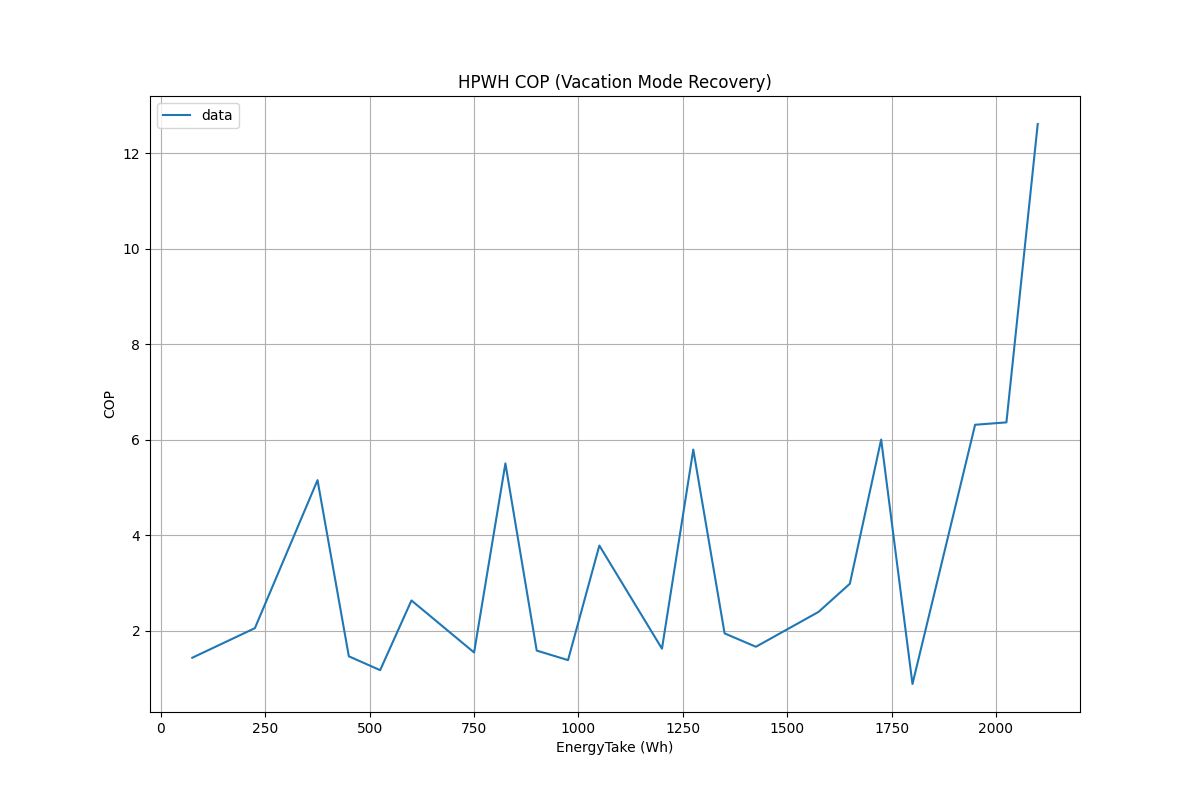
\includegraphics[width=0.9\columnwidth]{Pictures/cop_vs_EnergyTake_75.png}
    \caption{\gls{hpwh} COP vs EnergyTake: Vacation Mode Recovery}
    \label{fig:copET75}
\end{figure}
\newpage
\begin{figure}[ht!]
    \centering
    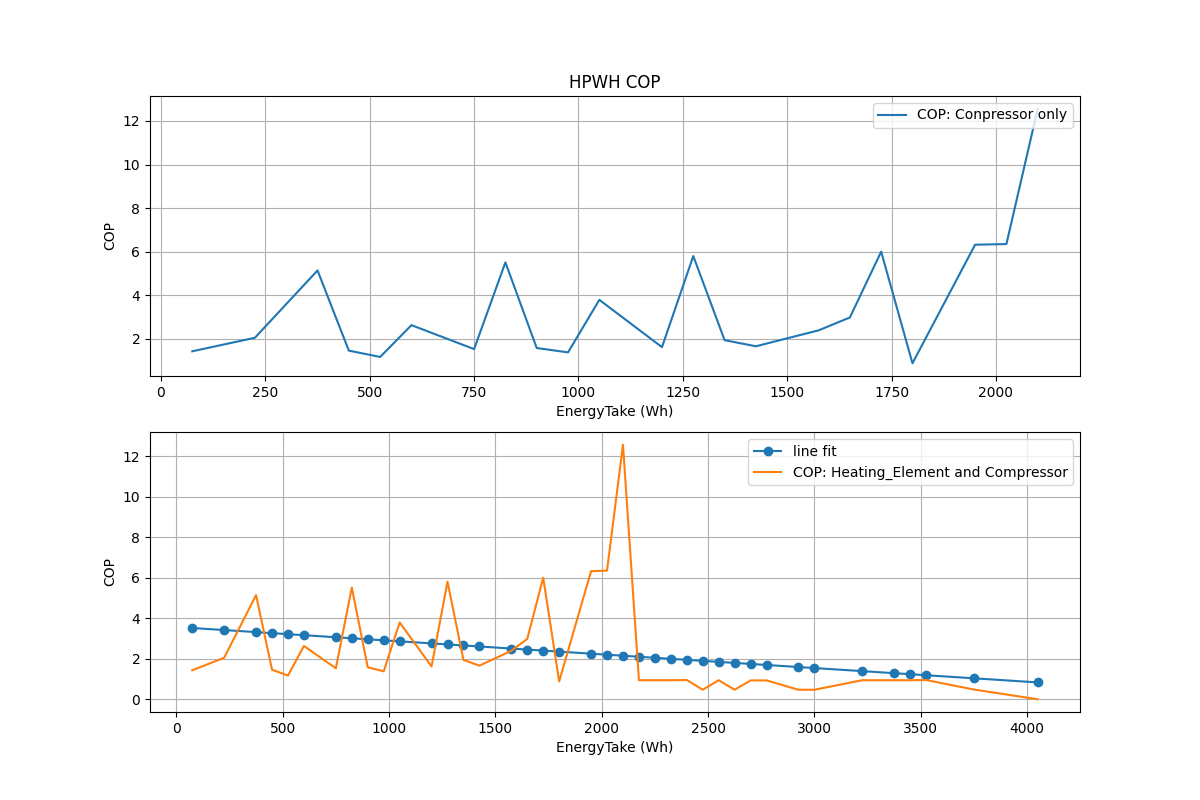
\includegraphics[width=\columnwidth]{Pictures/cop_vs_EnergyTake_75_linefit.png}
    \caption{\gls{hpwh} COP vs EnergyTake: Vacation Mode Recovery}
    \label{fig:copET75_linefit}
\end{figure}

\subsection{Oct 19}

The difference in EnergyTake in each timestemp was calculated. The data calculated is as shown in Table~\ref{table:EnergyTake Diff}
\begin{table}[ht!]
\caption{EnergyTake Difference Calculated}
\begin{adjustbox}{max width=\textwidth}
\begin{tabular}{|l|r|r|l|r|r|r|r|r|}
\hline
    time &  real\_available\_Wh &  consumed\_watts &   time.1 &  time\_diff &  average\_watts &   power in Wh&  EnergyTake\_diff &  cop \\ \hline

12:26:59 &               4050 &        4459.350 & 12:26:59 &       2.03 &        4459.35 &  150.87 &            300.0 & 1.99 \\ \hline
12:29:01 &               3750 &        4665.810 & 12:29:01 &       1.00 &        4665.81 &   77.76 &            225.0 & 2.89 \\ \hline
12:30:01 &               3525 &        4727.740 & 12:30:01 &       1.02 &        4727.74 &   80.37 &             75.0 & 0.93 \\ \hline
12:31:02 &               3450 &        4696.770 & 12:31:02 &       1.02 &        4696.77 &   79.85 &             75.0 & 0.94 \\ \hline
12:32:03 &               3375 &        4707.100 & 12:32:03 &       1.02 &        4707.10 &   80.02 &            150.0 & 1.87 \\ \hline
12:33:04 &               3225 &        4707.100 & 12:33:04 &       2.02 &        4707.10 &  158.47 &            225.0 & 1.42 \\ \hline
12:35:05 &               3000 &        4717.420 & 12:35:05 &       2.03 &        4717.42 &  159.61 &             75.0 & 0.47 \\ \hline
12:37:07 &               2925 &        4707.100 & 12:37:07 &       1.02 &        4707.10 &   80.02 &            150.0 & 1.87 \\ \hline
12:38:08 &               2775 &        4727.740 & 12:38:08 &       1.02 &        4727.74 &   80.37 &             75.0 & 0.93 \\ \hline
12:39:09 &               2700 &        4748.390 & 12:39:09 &       2.02 &        4748.39 &  159.86 &             75.0 & 0.47 \\ \hline
12:41:10 &               2625 &        4748.390 & 12:41:10 &       1.02 &        4748.39 &   80.72 &             75.0 & 0.93 \\ \hline
12:42:11 &               2550 &        4696.770 & 12:42:11 &       2.03 &        4696.77 &  158.91 &             75.0 & 0.47 \\ \hline
12:44:13 &               2475 &        4738.060 & 12:44:13 &       1.00 &        4738.06 &   78.97 &             75.0 & 0.95 \\ \hline
12:45:13 &               2400 &        4748.390 & 12:45:13 &       1.02 &        4748.39 &   80.72 &             75.0 & 0.93 \\ \hline
12:46:14 &               2325 &        4696.770 & 12:46:14 &       1.02 &        4696.77 &   79.85 &             75.0 & 0.94 \\ \hline
12:47:15 &               2250 &        4717.420 & 12:47:15 &       1.02 &        4717.42 &   80.20 &             75.0 & 0.94 \\ \hline
12:48:16 &               2175 &        4707.100 & 12:48:16 &       1.02 &        4707.10 &   80.02 &             75.0 & 0.94 \\ \hline
12:49:17 &               2100 &         350.968 & 12:49:17 &       2.02 &         350.97 &   11.82 &             75.0 & 6.35 \\ \hline
12:51:18 &               2025 &         350.968 & 12:51:18 &       2.03 &         350.97 &   11.87 &             75.0 & 6.32 \\ \hline
12:53:20 &               1950 &         350.968 & 12:53:20 &      14.18 &         350.97 &   82.95 &            150.0 & 1.81 \\ \hline
13:07:31 &               1800 &         361.290 & 13:07:31 &       2.02 &         361.29 &   12.16 &             75.0 & 6.17 \\ \hline
13:09:32 &               1725 &         371.613 & 13:09:32 &       4.07 &         371.61 &   25.21 &             75.0 & 2.98 \\ \hline
13:13:36 &               1650 &         371.613 & 13:13:36 &       5.07 &         371.61 &   31.40 &             75.0 & 2.39 \\ \hline
13:18:40 &               1575 &         371.613 & 13:18:40 &       7.08 &         371.61 &   43.85 &            150.0 & 3.42 \\ \hline
13:25:45 &               1425 &         381.935 & 13:25:45 &       6.08 &         381.94 &   38.70 &             75.0 & 1.94 \\ \hline
13:31:50 &               1350 &         381.935 & 13:31:50 &       2.03 &         381.94 &   12.92 &             75.0 & 5.80 \\ \hline
13:33:52 &               1275 &         381.935 & 13:33:52 &       7.08 &         381.94 &   45.07 &             75.0 & 1.66 \\ \hline
13:40:57 &               1200 &         392.258 & 13:40:57 &       3.03 &         392.26 &   19.81 &            150.0 & 7.57 \\ \hline
13:43:59 &               1050 &         392.258 & 13:43:59 &       8.12 &         392.26 &   53.09 &             75.0 & 1.41 \\ \hline
13:52:06 &                975 &         402.581 & 13:52:06 &       7.08 &         402.58 &   47.50 &             75.0 & 1.58 \\ \hline
13:59:11 &                900 &         402.581 & 13:59:11 &       2.03 &         402.58 &   13.62 &             75.0 & 5.51 \\ \hline
14:01:13 &                825 &         402.581 & 14:01:13 &       7.10 &         402.58 &   47.64 &             75.0 & 1.57 \\ \hline
14:08:19 &                750 &         412.903 & 14:08:19 &       4.05 &         412.90 &   27.87 &            150.0 & 5.38 \\ \hline
14:12:22 &                600 &         423.226 & 14:12:22 &       9.12 &         423.23 &   64.33 &             75.0 & 1.17 \\ \hline
14:21:29 &                525 &         423.226 & 14:21:29 &       7.10 &         423.23 &   50.08 &             75.0 & 1.50 \\ \hline
14:28:35 &                450 &         433.548 & 14:28:35 &       2.02 &         433.55 &   14.60 &             75.0 & 5.14 \\ \hline
14:30:36 &                375 &         433.548 & 14:30:36 &       5.07 &         433.55 &   36.63 &            150.0 & 4.10 \\ \hline
14:35:40 &                225 &         433.548 & 14:35:40 &       7.10 &         433.55 &   51.30 &            150.0 & 2.92 \\ \hline

\end{tabular}
\label{table:EnergyTake Diff}
\end{adjustbox}
\end{table}

\newpage

The data above was plotted as shown in the following figure. Note that the spike of COP = 12 has disappeared, which is progress, I guess. But Still the COP plot is not appropriate. The next steps that I have in mind is the following:

\begin{itemize}
    \item Plot the "EnergyTake diff" values versus time
    \item Fit a line into the data
    \item Repeate the same steps for the "power" values in the above table.
    \item Finally, caluclate the COP from the above lines.
\end{itemize}

The idea is that these spikes are caused by the fluctuating in the EnergyTake values (increment in 75 Wh). Averaging these values might be a solution to get a nice, clean plot.


\begin{figure}[htp!]
    \centering
    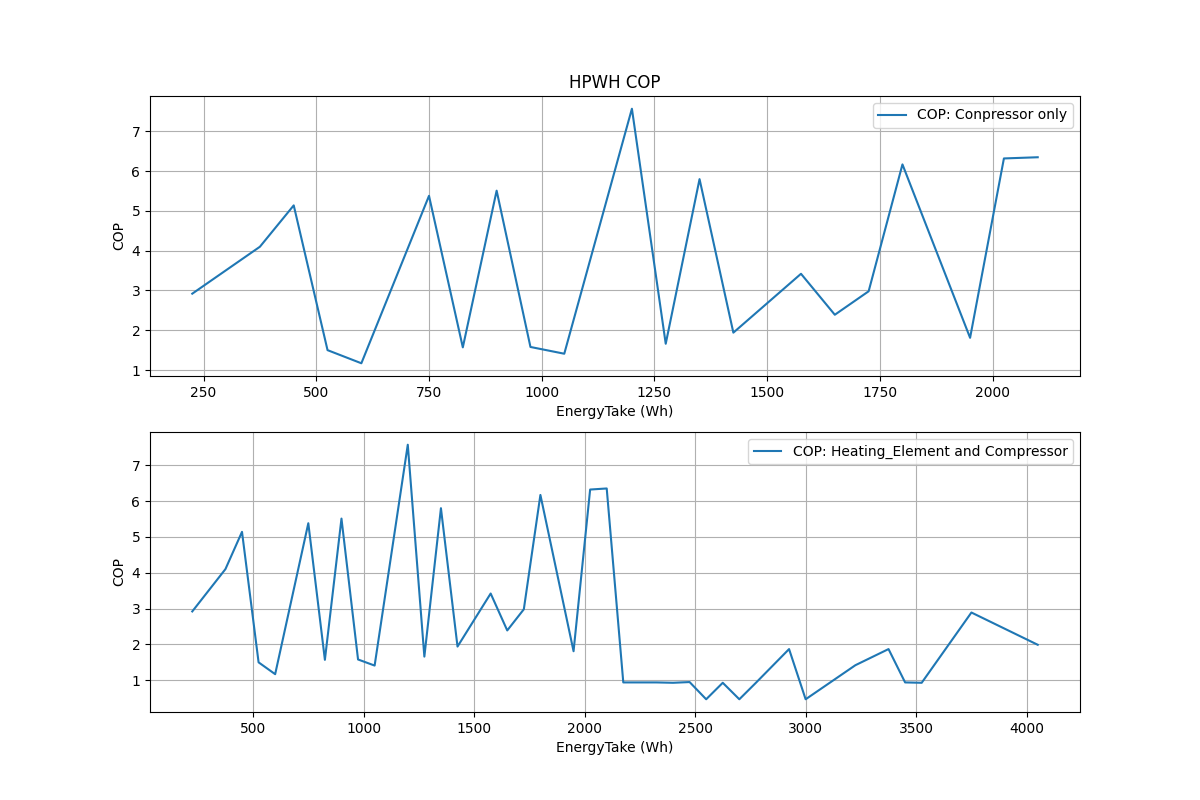
\includegraphics[width=0.9\columnwidth]{Pictures/cop_vs_EnergyTake_var.png}
    \caption{\gls{hpwh} COP vs EnergyTake: Vacation Mode Recovery}
    \label{fig:copET7_5}
\end{figure}

\subsection{Oct 26}

In this trial, I'm going to use the cumulative energy divided by the $Energy_{in}$. The $Energy_{in}$ is calculated as
following: (As coded in $cop\_vmode.py$ file)
\begin{itemize}
    \item Recorded the time difference between each timestep in a column named $time\_diff$
    \item Then each value in the $time\_diff$ column is converted to seconds (This is because timedelta library. It does
        not take arguments in minutes. It has to be seconds.)
    \item The seconds values is then converted to minutes and saved in the same column, $time\_diff$.
    \item Then the each value in the $time\_diff$ column is converted to hours by dividing the value by 60.
    \item Then the consumed power in each timestep ($consumed\_watts$ column) is multiplied by the time difference and
        saved in a new column named $energy\_in (Wh)$
\end{itemize}

The cumulative energy values is obvious which I believe there's no need to explain. However, for validation sake, each
csv file pulled from the DCS devices, contains a cumulative energy queries. These values are validated with the
calculated values.

The following table shows the data recorded for this simulation trial. Note that only the compressor operation is
recorded. The heating element operation was ignored in this table. 

\begin{table}[ht!]
\caption{Recorded and Calculated \gls{hpwh} Porperties}
\begin{adjustbox}{max width=\textwidth}
\begin{tabular}{|l|r|r|r|l|r|r|r|r|r|r|}
\hline
time &  cumulative\_energy &  real\_available\_Wh &  consumed\_watts &   time.1 &  EnergyTake\_diff &  time\_diff &  average\_watts &  power &  power\_cum &  cop \\ \hline

12:49:17 &                  0 &               2100 &         350.968 & 12:49:17 &             75.0 &       2.02 &         350.97 &  11.82 &       0.00 & 0.00 \\ \hline
12:51:18 &                 26 &               2025 &         350.968 & 12:51:18 &             75.0 &       2.03 &         350.97 &  11.87 &      11.82 & 2.20 \\ \hline
12:53:20 &                 52 &               1950 &         350.968 & 12:53:20 &            150.0 &      14.18 &         350.97 &  82.95 &      23.69 & 2.20 \\ \hline
13:07:31 &                234 &               1800 &         361.290 & 13:07:31 &             75.0 &       2.02 &         361.29 &  12.16 &     106.64 & 2.19 \\ \hline
13:09:32 &                260 &               1725 &         371.613 & 13:09:32 &             75.0 &       4.07 &         371.61 &  25.21 &     118.80 & 2.19 \\ \hline
13:13:36 &                312 &               1650 &         371.613 & 13:13:36 &             75.0 &       5.07 &         371.61 &  31.40 &     144.01 & 2.17 \\ \hline
13:18:40 &                390 &               1575 &         371.613 & 13:18:40 &            150.0 &       7.08 &         371.61 &  43.85 &     175.41 & 2.22 \\ \hline
13:25:45 &                481 &               1425 &         381.935 & 13:25:45 &             75.0 &       6.08 &         381.94 &  38.70 &     219.26 & 2.19 \\ \hline
13:31:50 &                559 &               1350 &         381.935 & 13:31:50 &             75.0 &       2.03 &         381.94 &  12.92 &     257.96 & 2.17 \\ \hline
13:33:52 &                585 &               1275 &         381.935 & 13:33:52 &             75.0 &       7.08 &         381.94 &  45.07 &     270.88 & 2.16 \\ \hline
13:40:57 &                676 &               1200 &         392.258 & 13:40:57 &            150.0 &       3.03 &         392.26 &  19.81 &     315.95 & 2.14 \\ \hline
13:43:59 &                715 &               1050 &         392.258 & 13:43:59 &             75.0 &       8.12 &         392.26 &  53.09 &     335.76 & 2.13 \\ \hline
13:52:06 &                819 &                975 &         402.581 & 13:52:06 &             75.0 &       7.08 &         402.58 &  47.50 &     388.85 & 2.11 \\ \hline
13:59:11 &                910 &                900 &         402.581 & 13:59:11 &             75.0 &       2.03 &         402.58 &  13.62 &     436.35 & 2.09 \\ \hline
14:01:13 &                936 &                825 &         402.581 & 14:01:13 &             75.0 &       7.10 &         402.58 &  47.64 &     449.97 & 2.08 \\ \hline
14:08:19 &               1027 &                750 &         412.903 & 14:08:19 &            150.0 &       4.05 &         412.90 &  27.87 &     497.61 & 2.06 \\ \hline
14:12:22 &               1079 &                600 &         423.226 & 14:12:22 &             75.0 &       9.12 &         423.23 &  64.33 &     525.48 & 2.05 \\ \hline
14:21:29 &               1196 &                525 &         423.226 & 14:21:29 &             75.0 &       7.10 &         423.23 &  50.08 &     589.81 & 2.03 \\ \hline
14:28:35 &               1287 &                450 &         433.548 & 14:28:35 &             75.0 &       2.02 &         433.55 &  14.60 &     639.89 & 2.01 \\ \hline
14:30:36 &               1326 &                375 &         433.548 & 14:30:36 &            150.0 &       5.07 &         433.55 &  36.63 &     654.49 & 2.03 \\ \hline
14:35:40 &               1391 &                225 &         433.548 & 14:35:40 &            150.0 &       7.10 &         433.55 &  51.30 &     691.12 & 2.01 \\ \hline
14:42:46 &               1482 &                 75 &         443.871 & 14:42:46 &             75.0 &       7.08 &         443.87 &  52.38 &     742.42 & 2.00 \\ \hline
14:49:51 &               1573 &                  0 &         443.871 & 14:49:51 &              0.0 &        NaN &         443.87 &    NaN &     794.80 & 1.98 \\ \hline

\end{tabular}
\label{table:cta-energytake}
\end{adjustbox}
\end{table}
\par As shown in table~\ref{table:cta-energytake}, the first cop values are zero because the cumulative energy is zero. The actual cop values
were NaN but they were converted to zero. Anyways, \textbf{The cumulative energy values are queries from the unit sent
using CTA2045}. The following table shows the calculated cumualtive energy which is the cumsum of the $EnergyTake\_diff$
column. These values are assigned in a new column that is called $EnergyTake\_cumsum$.


\subsection{Nov 16}

The calculated COP for this work is as shown in equation \ref{eq:cop_nov}

\begin{equation}\label{eq:cop_nov}
    COP = \frac{EnergyOut}{EnergyIn}
\end{equation}

The \textit{EnergyOut} is represented by the \textit{EnergyTake} gradient during the heating process. The \gls{hpwh} was set to \textit{efficiecy mode} and cooled down all the way to inlet water temperature. The heating element turned on for a while and then the compressor turned on. Since the operation of the heating element is predictable and its efficiency is understood, the COP was calculated for the compressor operation.

\subsubsection{Data Recorded}

During the heating process, several \gls{hpwh} properties were recorded and calculated as shown in Table~\ref{tab:cop_nov_table}. This section discusses the properties that were used to caluclate the COP. 

\begin{table}[ht!]
\caption{Recorded and Calculated \gls{hpwh} Porperties}
\begin{adjustbox}{max width=\textwidth}
\begin{tabular}{|r|r|r|l|r|r|r|r|r|r|r|r|}
\hline
 cumulative\_energy &  EnergyTake &  consumed\_watts &     time &  EnergyTake\_diff &  time\_diff &  average\_watts &  Energy\_in &  power\_cum &  ET\_fit\_comp &  W\_fit\_comp &  cop\_comp \\ \hline

                52 &               1950 &         350.968 & 12:53:20 &              150 &      14.18 &         350.97 &      82.95 &      23.69 &        94.70 &       34.47 &      2.75 \\ \hline
               234 &               1800 &         361.290 & 13:07:31 &               75 &       2.02 &         361.29 &      12.16 &     106.64 &        94.82 &       34.63 &      2.74 \\ \hline
               260 &               1725 &         371.613 & 13:09:32 &               75 &       4.07 &         371.61 &      25.21 &     118.80 &        95.06 &       34.95 &      2.72 \\ \hline
               312 &               1650 &         371.613 & 13:13:36 &               75 &       5.07 &         371.61 &      31.40 &     144.01 &        95.36 &       35.35 &      2.70 \\ \hline
               390 &               1575 &         371.613 & 13:18:40 &              150 &       7.08 &         371.61 &      43.85 &     175.41 &        95.78 &       35.91 &      2.67 \\ \hline
               481 &               1425 &         381.935 & 13:25:45 &               75 &       6.08 &         381.94 &      38.70 &     219.26 &        96.14 &       36.39 &      2.64 \\ \hline
               559 &               1350 &         381.935 & 13:31:50 &               75 &       2.03 &         381.94 &      12.92 &     257.96 &        96.26 &       36.55 &      2.63 \\ \hline
               585 &               1275 &         381.935 & 13:33:52 &               75 &       7.08 &         381.94 &      45.07 &     270.88 &        96.68 &       37.11 &      2.61 \\ \hline
               676 &               1200 &         392.258 & 13:40:57 &              150 &       3.03 &         392.26 &      19.81 &     315.95 &        96.86 &       37.35 &      2.59 \\ \hline
               715 &               1050 &         392.258 & 13:43:59 &               75 &       8.12 &         392.26 &      53.09 &     335.76 &        97.34 &       37.99 &      2.56 \\ \hline
               819 &                975 &         402.581 & 13:52:06 &               75 &       7.08 &         402.58 &      47.50 &     388.85 &        97.76 &       38.55 &      2.54 \\ \hline
               910 &                900 &         402.581 & 13:59:11 &               75 &       2.03 &         402.58 &      13.62 &     436.35 &        97.88 &       38.71 &      2.53 \\ \hline
               936 &                825 &         402.581 & 14:01:13 &               75 &       7.10 &         402.58 &      47.64 &     449.97 &        98.30 &       39.27 &      2.50 \\ \hline
              1027 &                750 &         412.903 & 14:08:19 &              150 &       4.05 &         412.90 &      27.87 &     497.61 &        98.54 &       39.59 &      2.49 \\ \hline
              1079 &                600 &         423.226 & 14:12:22 &               75 &       9.12 &         423.23 &      64.33 &     525.48 &        99.08 &       40.31 &      2.46 \\ \hline
              1196 &                525 &         423.226 & 14:21:29 &               75 &       7.10 &         423.23 &      50.08 &     589.81 &        99.50 &       40.87 &      2.43 \\ \hline
              1287 &                450 &         433.548 & 14:28:35 &               75 &       2.02 &         433.55 &      14.60 &     639.89 &        99.62 &       41.03 &      2.43 \\ \hline
              1326 &                375 &         433.548 & 14:30:36 &              150 &       5.07 &         433.55 &      36.63 &     654.49 &        99.92 &       41.43 &      2.41 \\ \hline
              1391 &                225 &         433.548 & 14:35:40 &              150 &       7.10 &         433.55 &      51.30 &     691.12 &       100.34 &       41.99 &      2.39 \\ \hline
              1482 &                 75 &         443.871 & 14:42:46 &               75 &       7.08 &         443.87 &      52.38 &     742.42 &       100.76 &       42.55 &      2.37 \\ \hline

\end{tabular}
\label{tab:cop_nov_table}
\end{adjustbox}
\end{table}

\subsubsection{\textit{EnergyTake} \& Energy\_in} 

The time (in minutes) that it takes the \gls{hpwh} to reports a change in the \textit{EnergyTake} (``EnergyTake\_diff'' column) and the power consumption (``avergae\_watts'' column) is shown in Table \ref{tab:cop_nov_table}, column ``time\_diff''. For each time window, the consumed watts is converted to energy and reported in the column ``Energy\_in''. As shown in the table, the ``Energy\_in'' values are proportional to the size of the time window. That is, as the time window increases, the ``Energy\_in'' values increase as well. 

\subsubsection{Linear line fitting}

A linear regression algorithm is used to fit lines to two plots. The first plot is the \textit{EnergyTake} VS Time, and the second plot is the \textit{Energy\_in} VS Time. Numpy Module in python provides an efficient way of doing such task by simply calling the function \textit{\textbf{polyfit}} along with equation's degree. Since our data behaves linearly, a polynomial equaiton with a degree of 1 was used to fit a line into each plot. Figure \ref{fig:line_fit} (Top) shows the \textit{EnergyTake} vs Time in minutes and the \textit{Energy\_in} along with a line to fit the data in each plot

\begin{figure}[htp!]
    \centering
    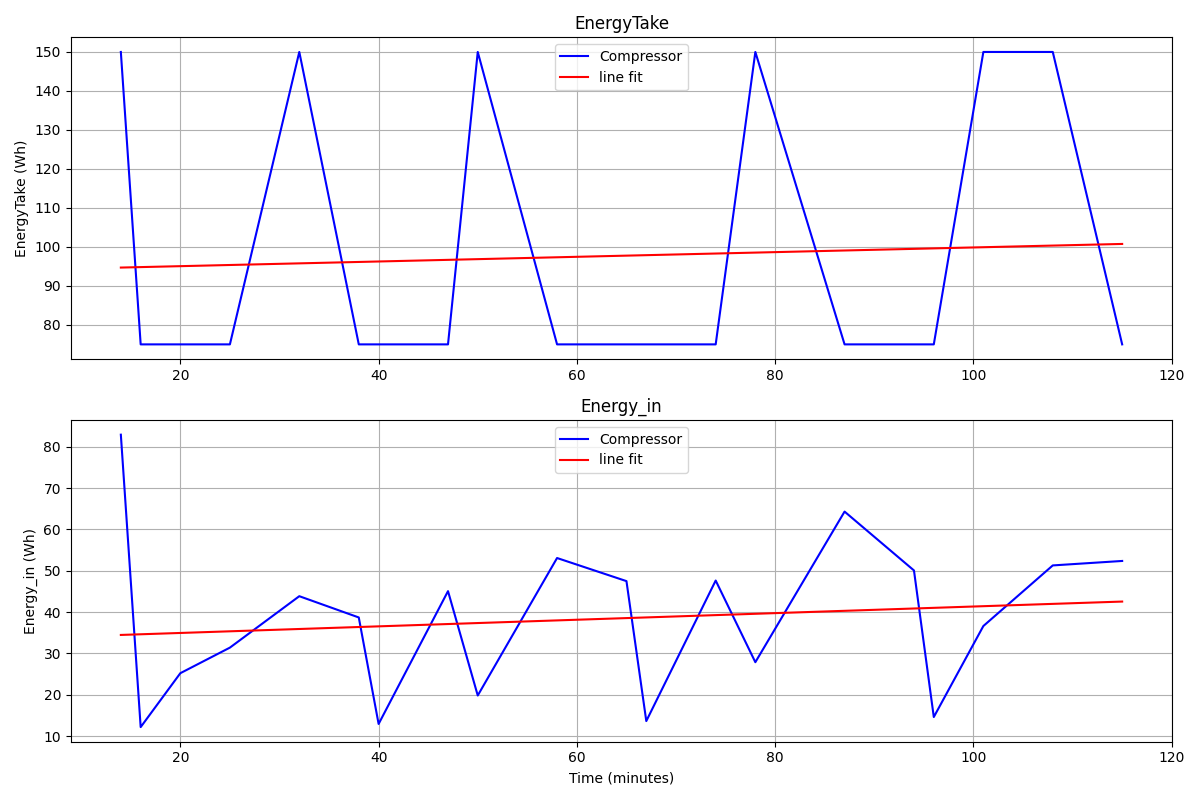
\includegraphics[width=0.9\columnwidth]{Pictures/energytake_watts_line_fit_nov.png}
    \caption{\gls{hpwh} EnergyTake (top) and Energy\_in (bottom) line fitting}
    \label{fig:line_fit}
\end{figure}

\subsubsection{COP}

The COP is calculated as shown in Equation \ref{eq:cop_nov}. The EnergyOut is the ``EnergyTake\_diff'' column shown in Table \ref{tab:cop_nov_table} and the EnergyIn is the ``EnergyIn'' column shown in Table \ref{tab:cop_nov_table}. The lines fit of each of the represented data were used to calculate the COP. The COP ranges between 2.3 and 2.76 as shown in Figure \ref{fig:cop_nov}

\begin{figure}[htp!]
    \centering
    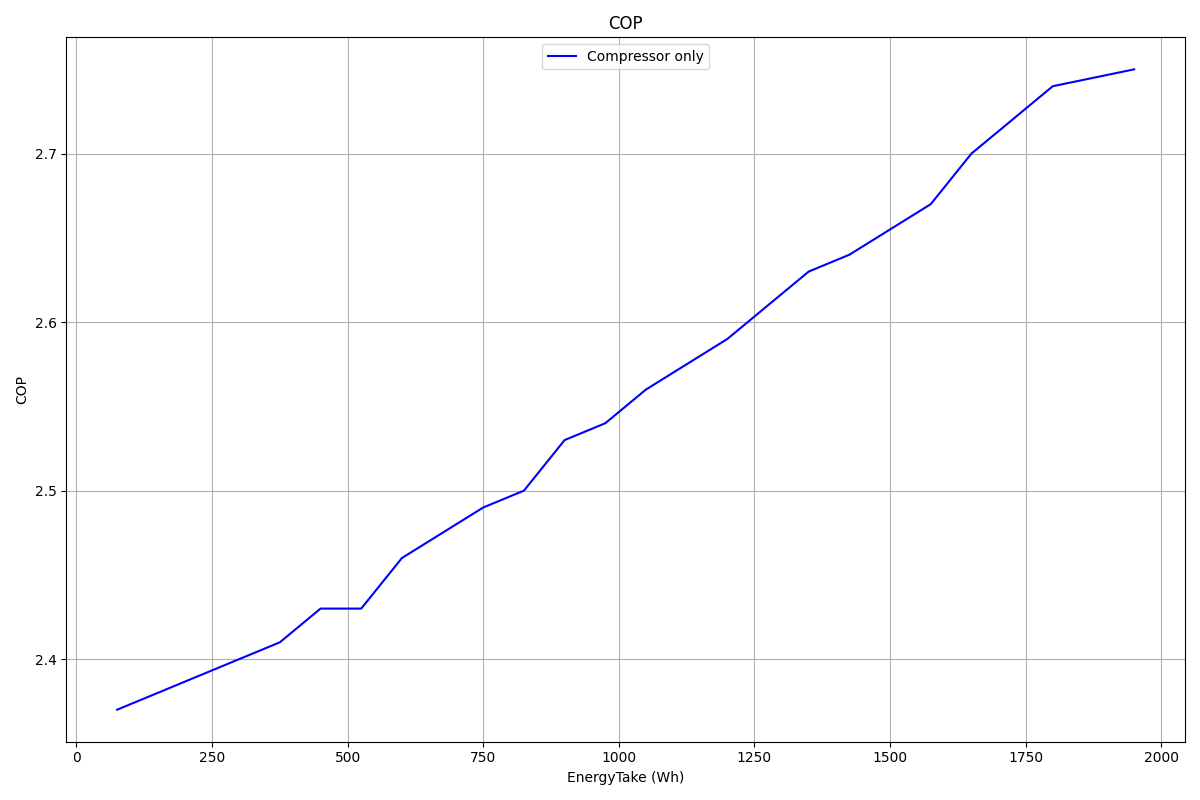
\includegraphics[width=0.9\columnwidth]{Pictures/cop_nov.png}
    \caption{\gls{hpwh} COP vs EnergyTake: Vacation Mode Recovery}
    \label{fig:cop_nov}
\end{figure}

Therefore, the equation for the COP is as follows:

\begin{equation}\label{eq:cop_nov_lines_fit}
    COP = \frac{0.06 \times \textit{EnergyTake} + 93.86}{0.08 \times \textit{EnergyIn} + 33.35}
\end{equation}

\newpage

\subsubsection{Relationship between Power Consumption (W) and \textit{EnergyTake} (Wh)}

This relationship is needed when the \textit{EnergyTake} changes due to the triggering of the heating source, either the heating element or the compressor. To get an equation that is representative for this relationship, both maximum compressor threshold points of the compressor and the heating element are considered. From the \gls{emcb} use cases report, case 3, the 20 gallon water draw event caused the \textit{EnergyTake} to increase more than 2000~Wh. The heating element triggered and heated the water until the \textit{EnergyTake} reached 200~Wh. The heating element then switched off and the compressor triggered to heat the water until the set points. Therefore, two equations are needed to represent this behavior. One for the heating element operation, and one for the compressor operation. 

For the compressor operation, the \textit{EnergyTake} data were plotted against the power consumption as shown in Figure~\ref{fig:w_wh_comp}. The same process is repeated for the heating element as shown in Figure~\ref{fig:w_wh_heating_elem}. To get a representative equation for the compressor and heating element, a line-fit equation was fit to both curves. 

\begin{figure}[htp!]
    \centering
    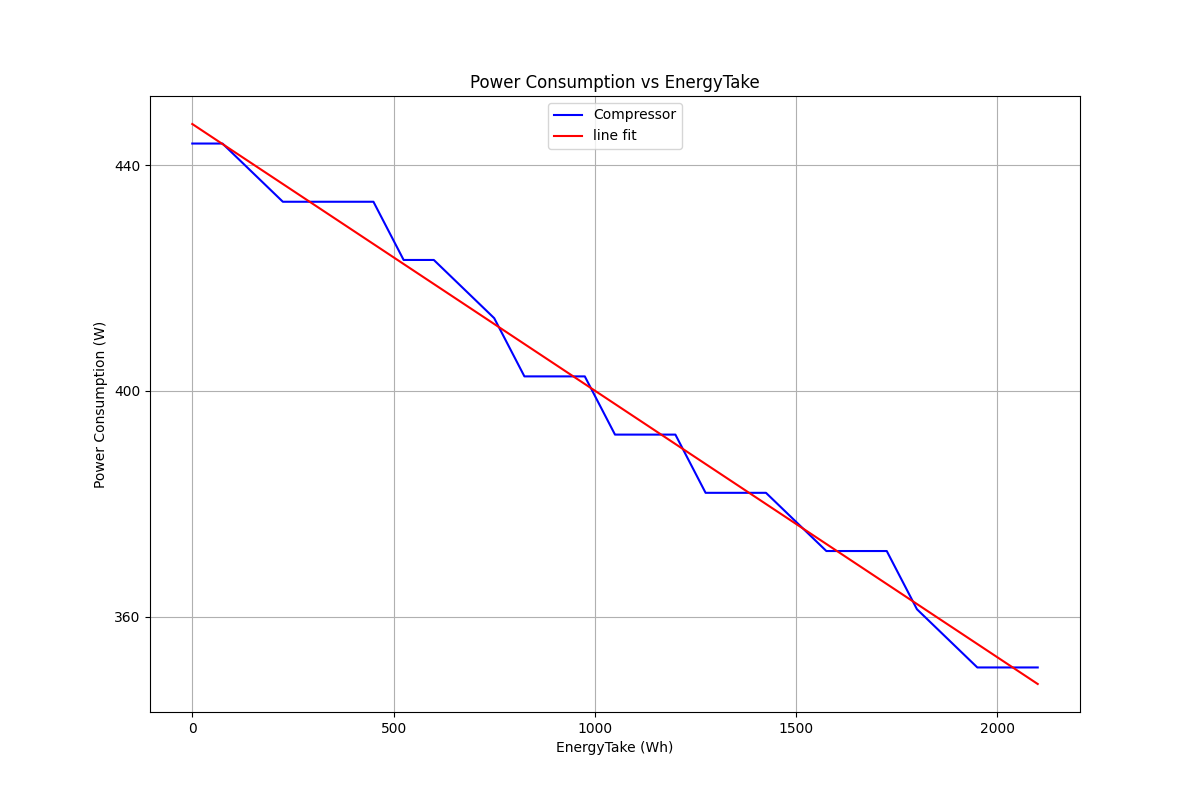
\includegraphics[width=0.99\columnwidth]{Pictures/watts_wh_relation_comp.png}
    \caption{\gls{hpwh} Watts vs EnergyTake: Vacation Mode Recovery}
    \label{fig:w_wh_comp}
\end{figure}

\begin{figure}[htp!]
    \centering
    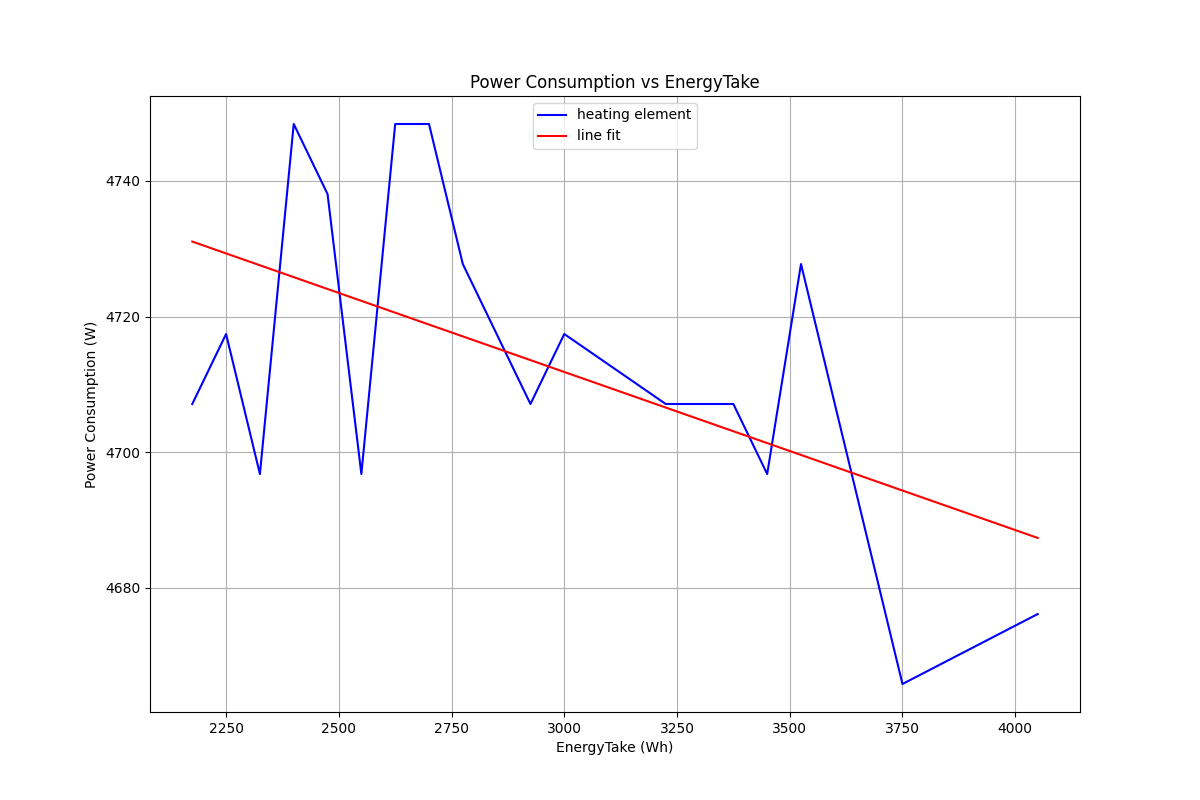
\includegraphics[width=0.99\columnwidth]{Pictures/watts_wh_relation_heating_element.png}
    \caption{\gls{hpwh} Watts vs EnergyTake: Vacation Mode Recovery}
    \label{fig:w_wh_heating_elem}
\end{figure}

\newpage

\subsubsection{HPWH Idle Losses}
To test the change in \textit{EnergyTake} when the \gls{hpwh} is idle, a \textit{CPE} command was sent and no water draws were applied. The \gls{hpwh} was allowed to cool down all the way to 1600~Wh as shown in Figure~\ref{fig:hpwh_idle_losses}.
\begin{figure}[htp!]
    \centering
    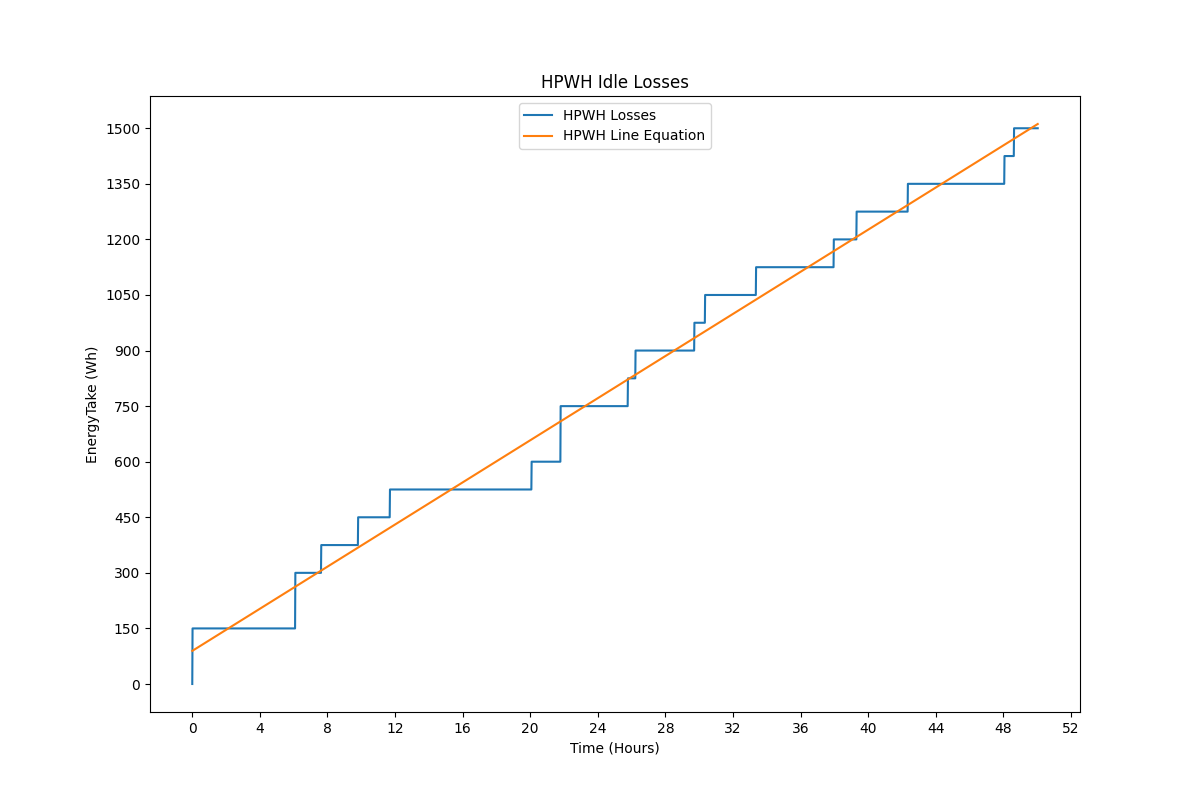
\includegraphics[width=0.99\columnwidth]{Pictures/hpwh_idle_losses.png}
    \caption{\gls{hpwh} EnergyTake vs Time: Vacation Mode Recovery}
    \label{fig:hpwh_idle_losses}
\end{figure}

\newpage

\subsubsection{Power Consumption (W) and \textit{EnergyTake} (Wh) Validation Test}

The compressor behavior is modeled using the following equation:

\begin{equation}\label{eq:cop_nov_lines_fit_}
    P(ET) = -0.04729 \times ET + 447.3
\end{equation}

The heating element behavior is modeled using the following equation:


\begin{equation}\label{eq:cop_nov_lines_fi_t}
    P(ET) = -0.02331 \times ET + 4782
\end{equation}

Both of these equations were tested against the \gls{emcb} data. Their behavior is shown in Figure~\ref{fig:hpwh_idle_losses}.

\begin{figure}[htp!]
    \centering
    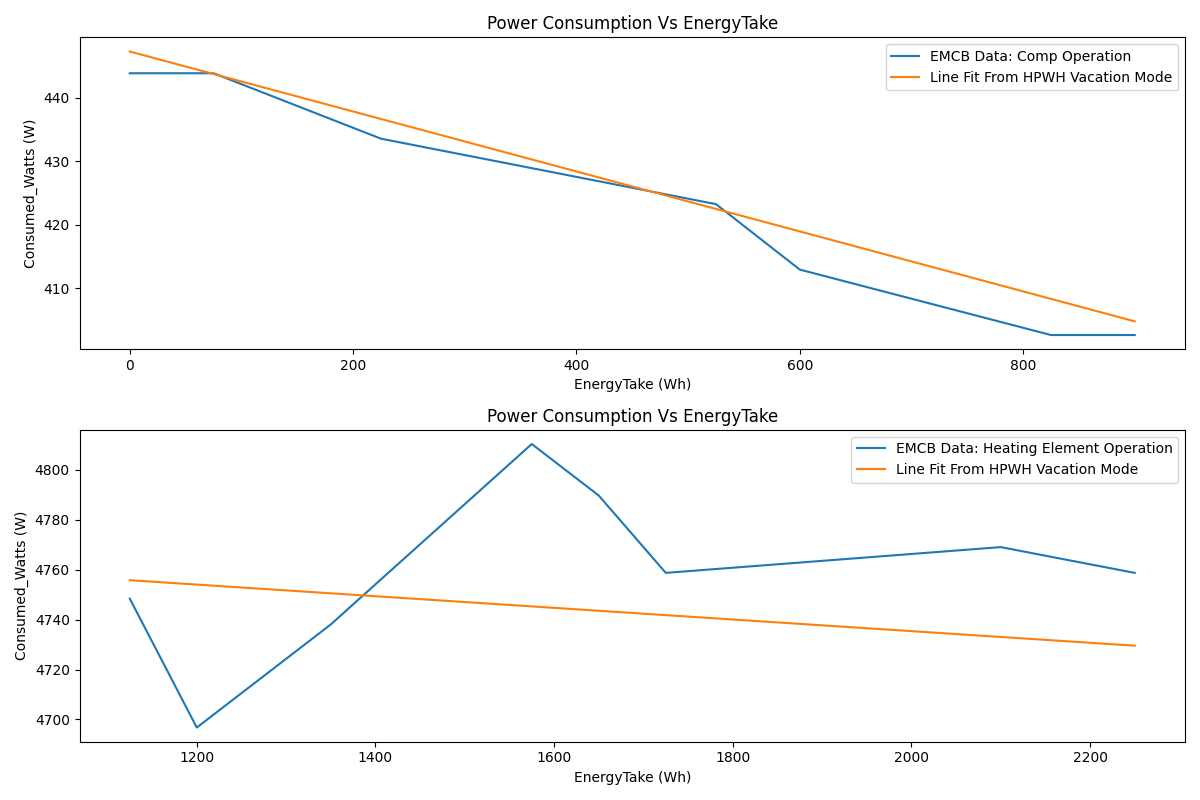
\includegraphics[width=0.9\columnwidth]{Pictures/w_wh_validation.png}
    \caption{\gls{hpwh} Watts vs EnergyTake: Validation with \gls{emcb} Data}
    \label{fig:hpwh_idle_l_osses}
\end{figure}
\newpage
\subsubsection{HPWH Idle Losses Validation Test}
The idle losses equation was also tested agains the \gls{emcb} data. Since the equation was created from a operiod of two days, the equaiton did not perform well with the testing data. Therefore, a modification factor was added to the equation. The modification factor was obtained upon different testings. Figure~\ref{fig:hpwh_idle_losses_val} shows the behavior of Equation~\ref{eq:idle_losses_lines_fit_modified} when tested with the \gls{emcb} data.

The original equation:

\begin{equation}\label{eq:idle_losses_lines_fit_original}
    E(time) = 0.4737 \times time + 89.36
\end{equation}

The modified equation:

\begin{equation}\label{eq:idle_losses_lines_fit_modified}
    E(time) = 0.8960 \times time + 126
\end{equation}

\newpage
\begin{figure}[ht]
    \centering
    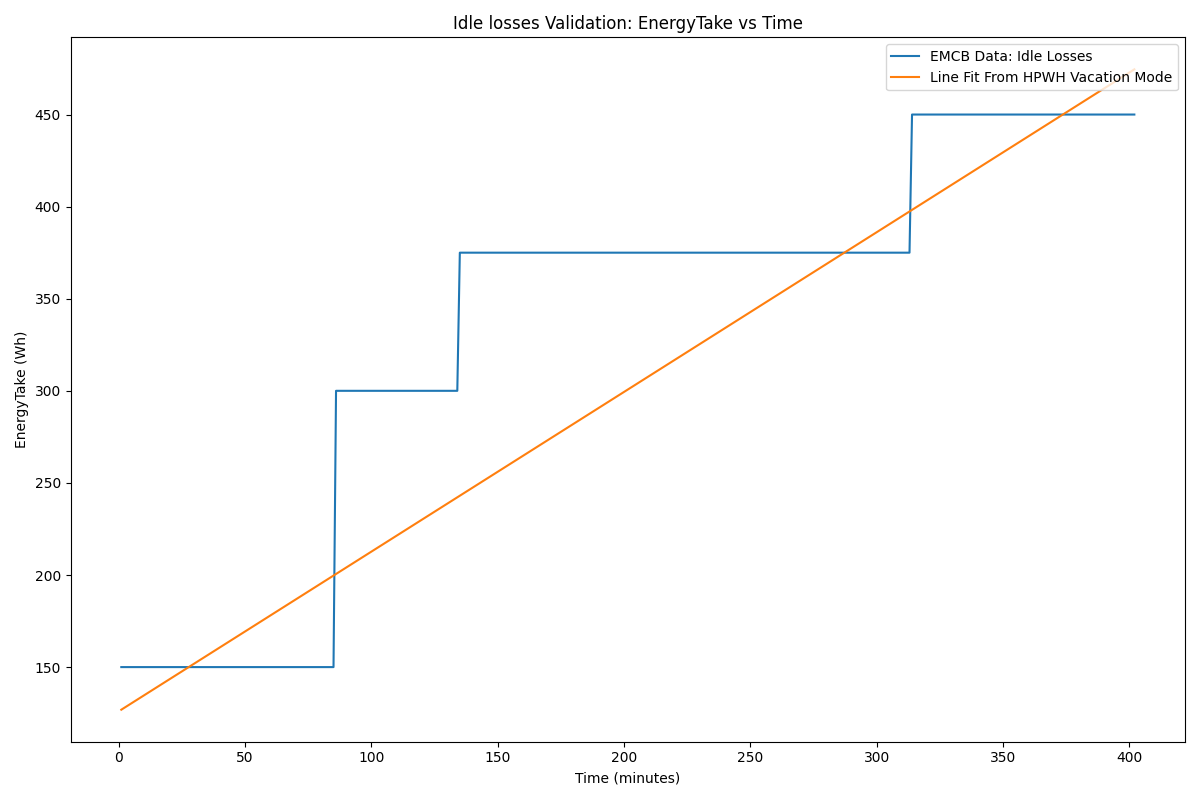
\includegraphics[width=0.9\columnwidth]{Pictures/idle_losses_val_validation.png}
    \caption{\gls{hpwh} Idle losses: Validation with \gls{emcb} Data}
    \label{fig:hpwh_idle_losses_val}
\end{figure}

\newpage
\subsubsection{\textit{EnergyTake} as a function of Water Draw Volume}

As water draw occurs, the temperature in the tank changes due to influx water. The influx water is the water entering the tank due to water leaving the tank. The influx water temperature is usually around 60${^\circ}F$. In this test, I'm trying to measure the temperature of the tank as a 20~gallon water volume enters the tank and gets mixed with 30~gallon water in the tank.

As the cold water enters the tank, the heat in the hot water transfers to the cold water and vice-versa. This process continues to happen until both water volumes reach the same temperature. In other words, the hot water loses heat and cold water gains heat. This can be interperted from the first law of thermodynamics: Energy Conservation. This process can be expressed mathematically as shown in equation~\ref{eq:heat_transfer}, where $Q_{lost}$ and $Q_{gain}$ are expressed as shown in equations~\ref{eq:qlost} and ~\ref{eq:qgain}. Equating equations~\ref{eq:qlost} and~\ref{eq:qgain} and solving for $T_{New}$, we end up with equation~\ref{eq:Tnew}

\begin{equation}\label{eq:heat_transfer}
    Q_{lost} = Q_{gained}
\end{equation}

\begin{equation}\label{eq:qlost}
    Q_{lost} = V_{WaterTank} (gal) \times \rho_{water} (\frac{lb}{gal}) \times C_{p} (\frac{Btu}{lb.F}) \times (T_{Set point} - T_{New})
\end{equation}

\begin{equation}\label{eq:qgain}
    Q_{gain} = V_{WaterDraw} (gal) \times \rho_{water} (\frac{lb}{gal}) \times C_{p} (\frac{Btu}{lb.F}) \times (T_{New} - T_{init})
\end{equation}

\begin{equation}\label{eq:Tnew}
    T_{New} = \frac{(V_{WaterTank} \times T_{Set point}) + (V_{Draw} \times T_{inlet})}
    {V_{draw} + V_{WaterTank}}
\end{equation}

\newpage

Equation~\ref{eq:Tnew} approximates the temperature of the tank after both water volumes get mixed together. As the \gls{hpwh} model detects the drop in the temperature, one of the heating elements will trigger to heat the water. The change in temperature as heat added to the tank is calculated as shown in equation~\ref{eq:Tchange}. Keep in mind that the heat added to the tank is now heating the whole 50~gallon.

\begin{equation}\label{eq:Tchange}
    \Delta T = \frac{(Q_{added} (btu))}
    {(C_{p} (\frac{Btu}{lb.F}) \times V_{WaterTank} (gal) \times \rho_{water} (\frac{lb}{gal}))}
\end{equation}
\newline


Where $Q_added$ is as follows:

\begin{equation}\label{eq:Tchang_e}
    Q_{added} (btu) = P_{consumed} (W) \times T_{step} (h) * 3.41
\end{equation}

\subsubsection{Testing}

The above procedure was tested on one of the \gls{emcb} files. The water draw event was 20~gallon. Table~\ref{tab:temp_comp} shows comparison between the calculated temperature (inferred from ET) and the temperature calculated from the above equations.

\begin{table}[ht]
\centering
\caption{Temperature Comparison}
\begin{adjustbox}{max width=\textwidth}
\begin{tabular}{|r|r|}
\hline
 Original Temp &   Calc\_Temp \\ \hline
     97.029769 &  101.557377 \\ \hline
     98.059539 &  102.786885 \\ \hline
    101.148847 &  105.860656 \\ \hline
    103.208385 &  106.475410 \\ \hline
    104.238155 &  107.090164 \\ \hline
    107.327463 &  108.934426 \\ \hline
    109.387001 &  110.163934 \\ \hline
    110.416770 &  110.778689 \\ \hline
    112.242271 &  112.622951 \\ \hline
    112.698646 &  113.237705 \\ \hline
    114.372021 &  115.081967 \\ \hline
    115.589021 &  115.696721 \\ \hline
    117.870896 &  118.155738 \\ \hline
    119.087896 &  119.385246 \\ \hline
    120.000646 &  119.779253 \\ \hline
\end{tabular}
\label{tab:temp_comp}
\end{adjustbox}
\end{table}

\begin{comment}
The \gls{hpwh} model reports the \textit{EnergyTake} according to the timestamp specified by the user. For this test, the timestamp is assumed to be one minute. Also, we're assuming that the water draw for this experiment is 20~Gallon. To calculate the change in the \textit{EnergyTake} corresponding to the 20~Gallon water draw, the \textit{EnergyTake} of the tank is calculated when 20~Gallon hot water is replaced with 20~Gallon cold water. 

\begin{equation}\label{eq:et_water_draw}
    Q = V_{WaterDraw} (gal) \times \rho_{water} (\frac{lb}{gal}) \times C_{p} (\frac{Btu}{lb.F}) \times (T_{avg} - T_{init})
\end{equation}

The parameters in Equation~\ref{eq:et_water_draw} are defined as follows:
\begin{itemize}
    \item $\rho_{water}$ = 8.3176 $\frac{lb}{gal}$
    \item $C_{p}$ = 0.998 $\frac{Btu}{lb.F}$
    \item $V_{WaterDraw}$ = 20 gallon
    \item $T_{avg}$ = 101.76 $^{\circ}$F
    \item $T_{init}$ = 60 $^{\circ}$F
\end{itemize}

The result of Equation~\ref{eq:et_water_draw} indicates the energy in the tank after mixing the cold water with hot water, which is 6899.26 btu. Converting Q to Wh by multiplying by 0.293, we end up with 2021.48~Wh. For the same conditions, the \gls{dcs} reports \textit{EnergyTake} of 2250~Wh. This difference between the calculated values and measured values is repeated through other experiments. Therefore, a correction factor of 1.113 is multiplied by the heat value (2021.48~Wh) gives us 2249.91, which reflects the measured values accurately. 

Two more steps are needed to be taken to achieve a good \texit{EnergyTake} model. One is to continue the \textit{EnergyTake} calculations until 0~Wh is reached. Second is to find a ramp rate that indicate the impact of the 20~gallon water gradually instead of an instantenous response as shown above. For the former, the temperature
\end{comment}

\begin{comment}
\subsection{Temperature Calculations}

\subsubsection{\gls{hpwh} Behavior \& Assumptions}

Before we get into temperature calculations, let's get a general idea of how the \gls{hpwh} behaves when the temperature decreases. A long with the compressor, the \gls{hpwh} has two heating elements, one at the top of the tank, and one near the bottom of the tank. My focus is on the compressor and the upper heating element. In case of an aggressive water draw that increases the \textit{EnergyTake} to 2000~Wh, the upper heating element triggers.\footnote{Look at the \gls{emcb} report, test case analysis no. 3 \& 4.} 

L. Clarke~\cite{LeightonClarke} used five sensors in the \gls{ewh} to measure the temperature inside the tank as shown in Figure~\ref{fig:temp_data} during a water draw, aggressive one, I believe. The sensors are arranged from one to five, top to bottom. Note that during the water draw event, the top two sensors did not record much change in the temperature. However, the lower three sensors recorded a significant drop in the temperature. This shows different layers of thermal stratification within the tank. Caclaulating the temperature in the \gls{hpwh} would require similar process.

\begin{figure}[H]
    \centering
    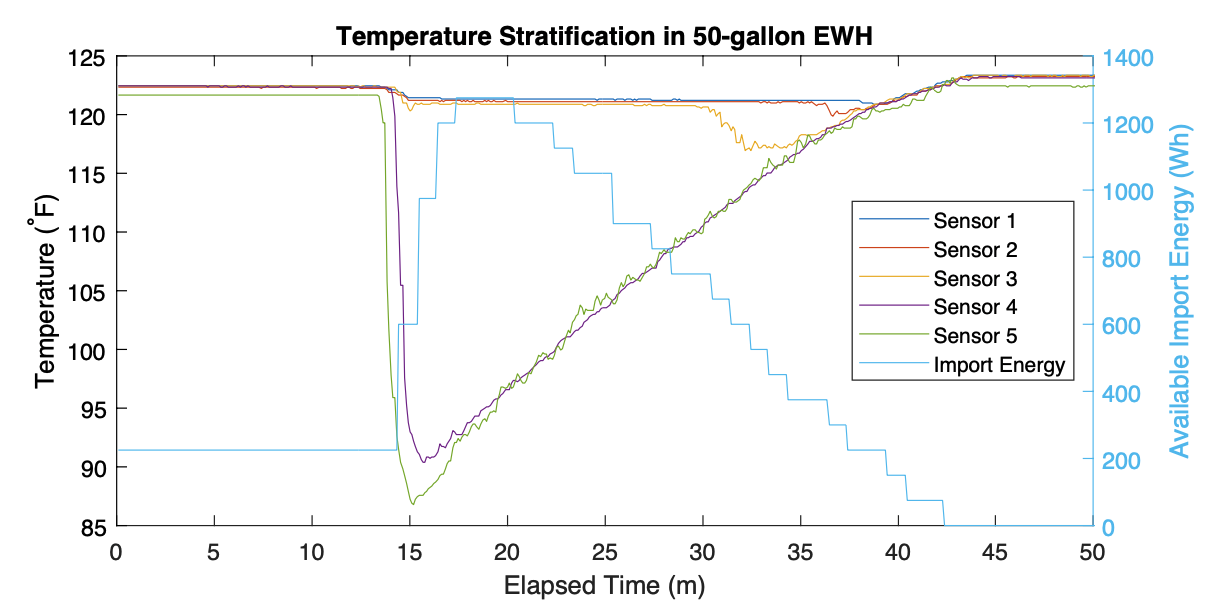
\includegraphics[width=0.9\columnwidth]{Pictures/temp_sensors_data.png}
    \caption{EWH Temperature Sensors Data~\cite{LeightonClarke}}
    \label{fig:temp_data}
\end{figure}
\newpage

L. Clarke~\cite{LeightonClarke} planted the sensors in the \gls{ewh} by replacing the anode rode with five sensors. In the \gls{hpwh} case, the anode rode is not accessible. In fact, even if it were accessible, it'd require un-installing the water heater station due to lack of space between the top of the station and the roof. Furthermore, the \gls{hpwh} has internal sensors that measure the temperature of the water. However, these sensors are, also, not accessible and they're used for logic control within the tank. For the previous reasons, the best way to approach an average temperature results is by considering the \textit{EnergyTake}. The \gls{hpwh} uses unknown controlling logic to calculate the \textit{EnergyTake} values and reports them through \acrshort{cta}-2045. 

The temperature calcualtions used in this work is in Rankine scale. The reason for that is the \textit{EnergyTake} is in Watts-hour. The corresponding temperature for a zero Wh \textit{EnergyTake} is also $0^{\circ} R$.

\end{comment}


\pagebreak

\newpage
\section{Winter 2022}
% \label{Winter2022}
\subsection{GridLAB-D Model Validation}
\textbf{THIS SECTION AND FORWARD NEEDS TO BE REWRITTEN AND EXPLAINED. FOR NOW, I'M POSTING IMAGES HERE TO PRESENT IN THE TECH MEETING}
\newpage
\subsubsection{HPWH Water Demand Behavior}
\begin{figure}[H]
    \centering
    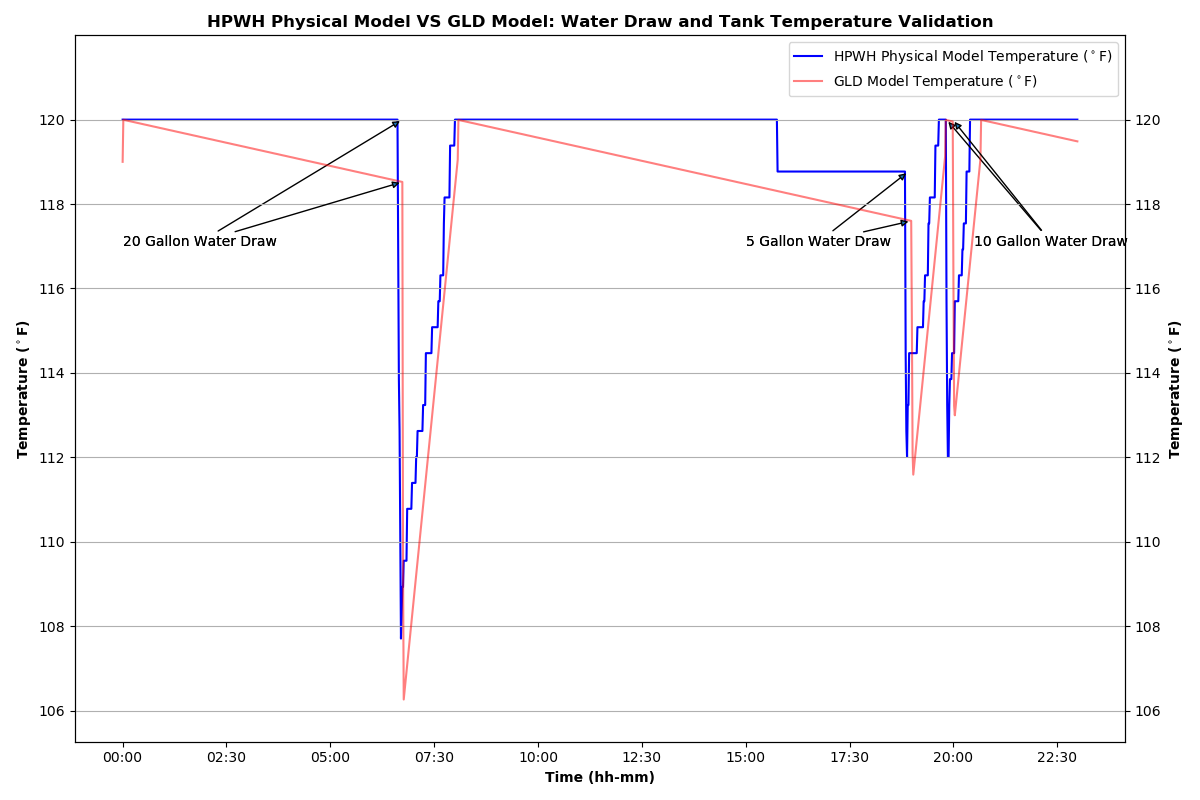
\includegraphics[width=1.1\columnwidth]{Pictures/Temperature_validation.png}
    \caption{GLD and Physical Model Validation: Water Draw Validation}
    %\label{fig:temp_data}
\end{figure}

\newpage
\subsubsection{Idle Losses}
\begin{figure}[H]
    \centering
    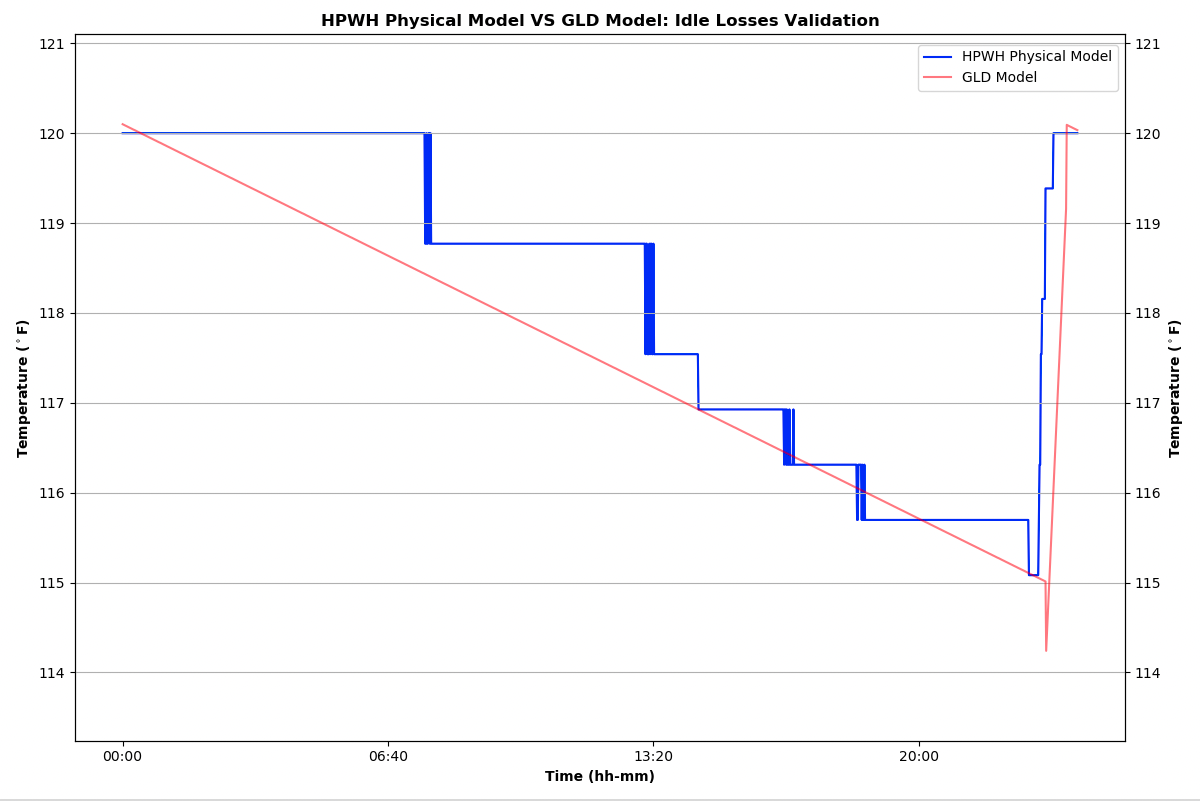
\includegraphics[width=1.1\columnwidth]{Pictures/idle_losses.png}
    \caption{GLD and Physical Model Validation: Idle Losses}
    %\label{fig:temp_data}
\end{figure}

\newpage
\subsubsection{Heating Sources Switching}
\begin{figure}[H]
    \centering
    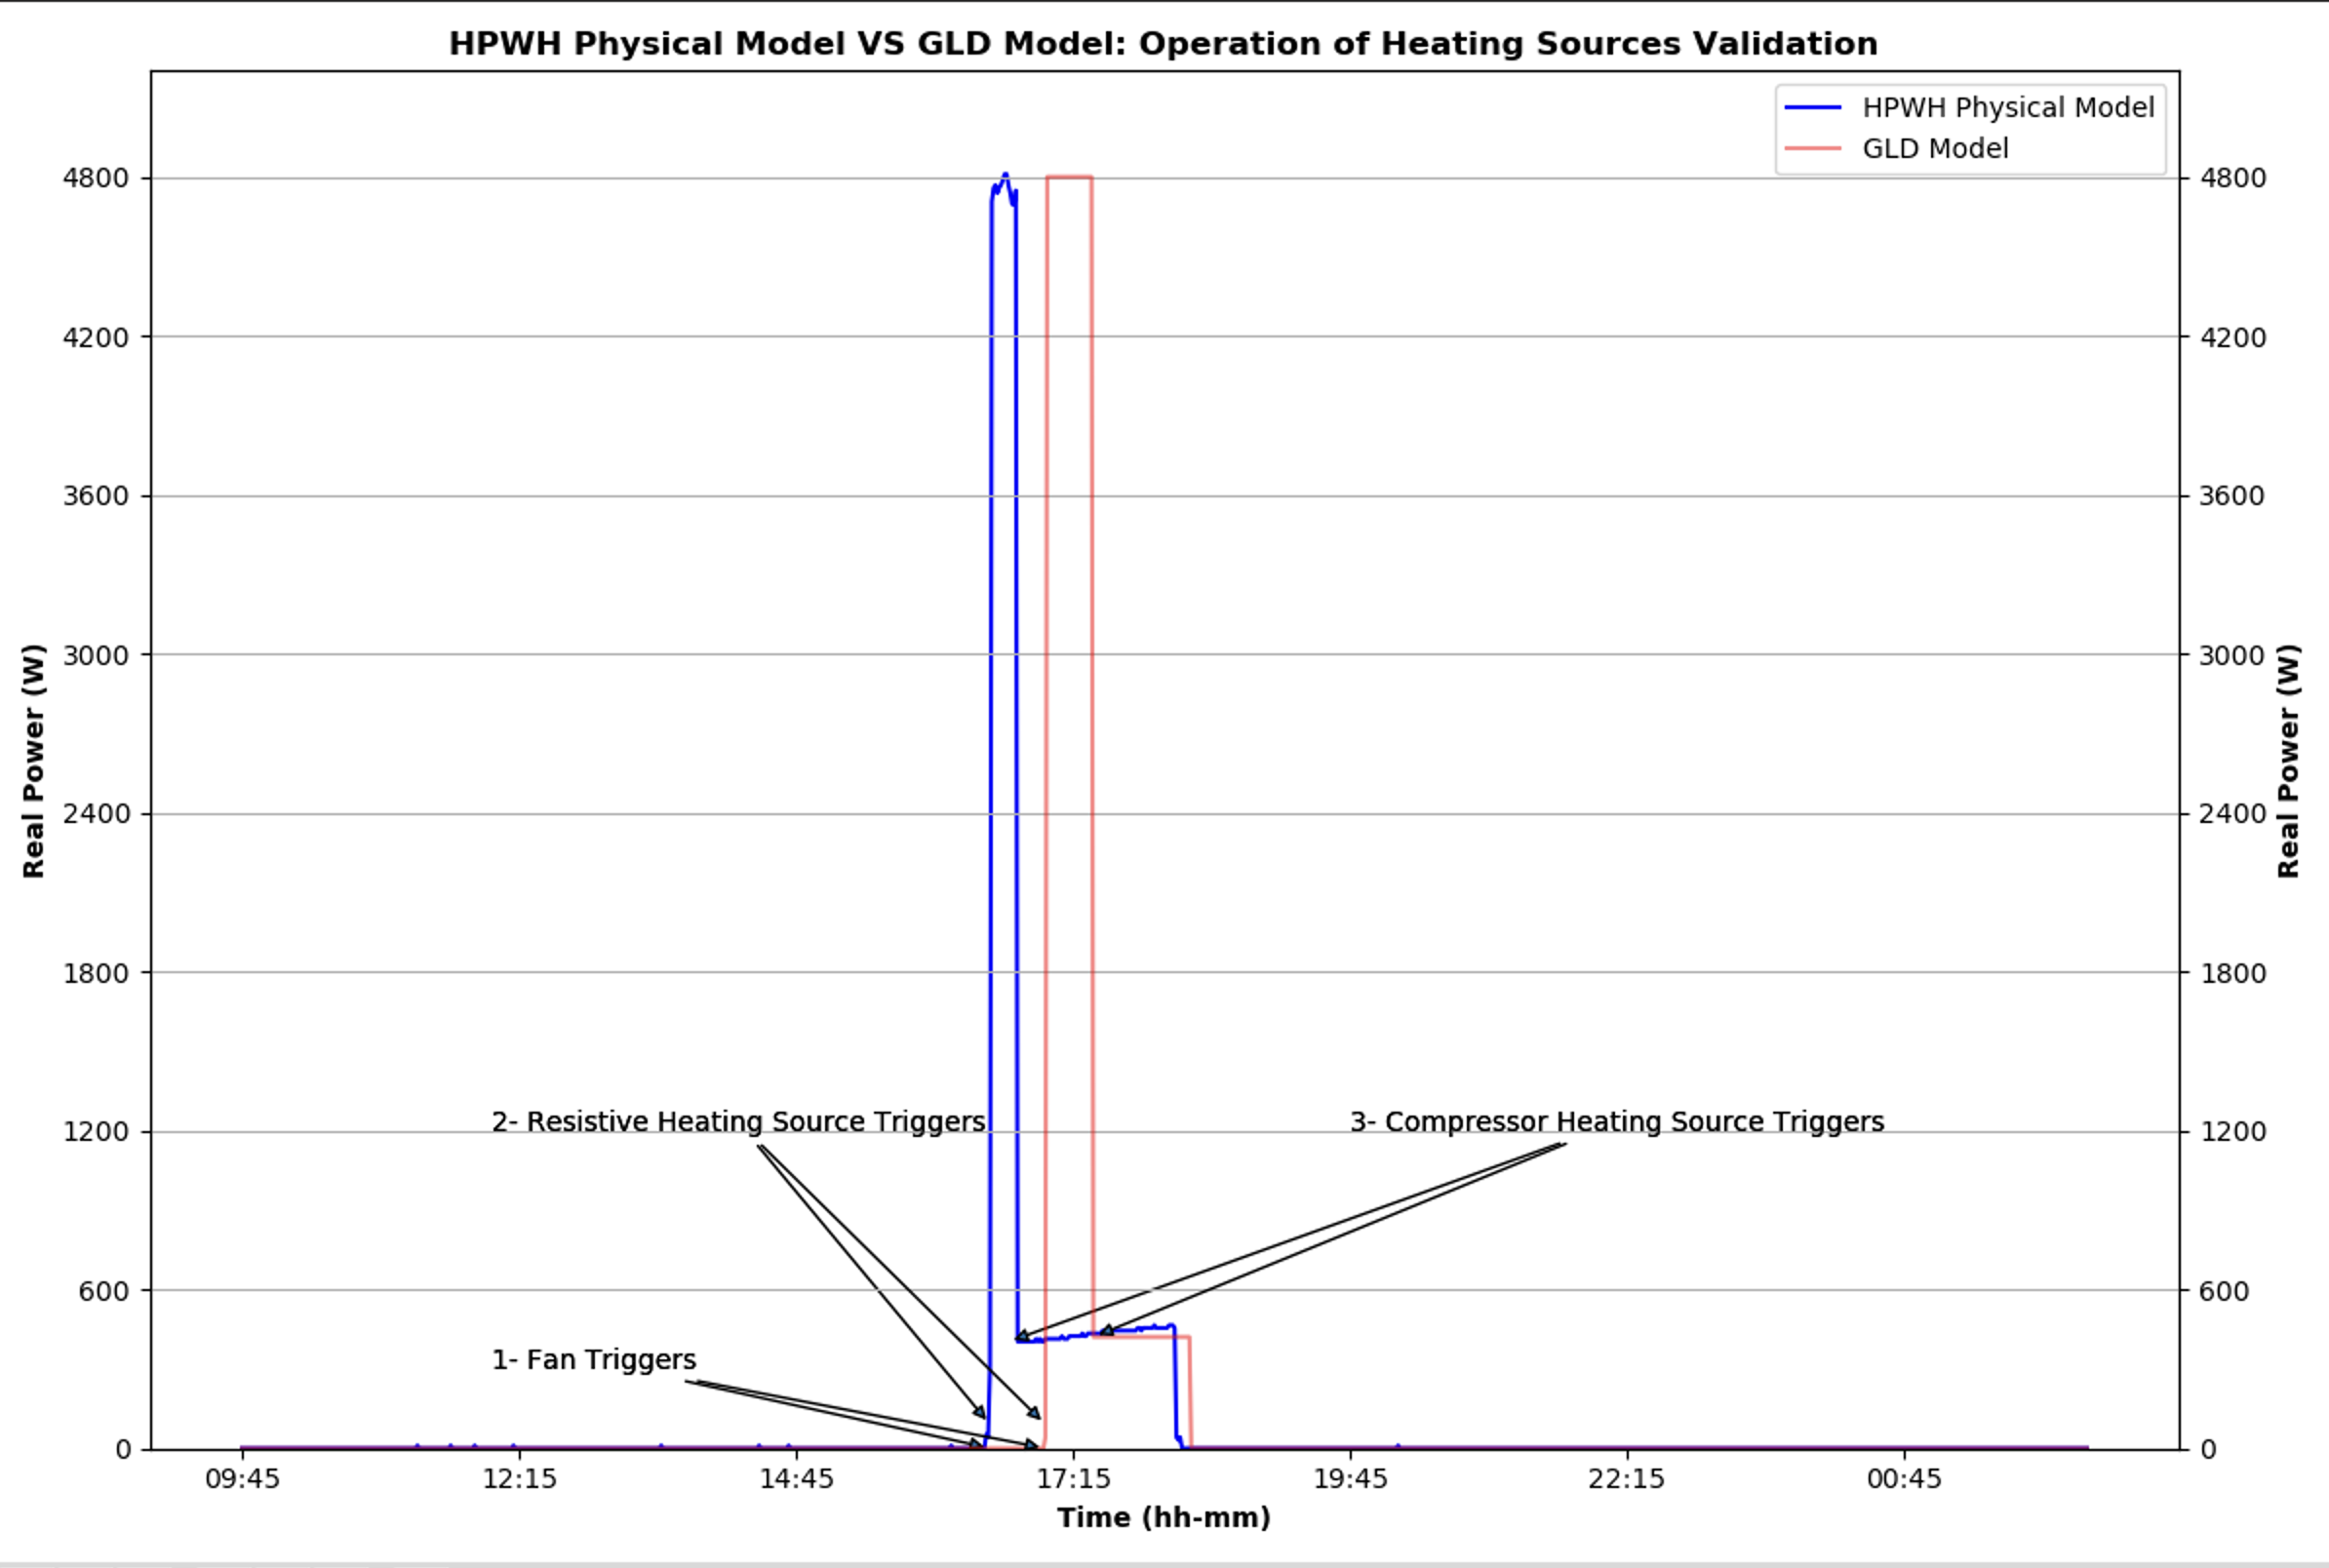
\includegraphics[width=1.1\columnwidth]{Pictures/heating_element_switching.png}
    \caption{GLD and Physical Model Validation: Heating Sources Switching}
    %\label{fig:temp_data}
\end{figure}
\newpage
\subsubsection{Data Samples}
\begin{figure}[H]
    \centering
    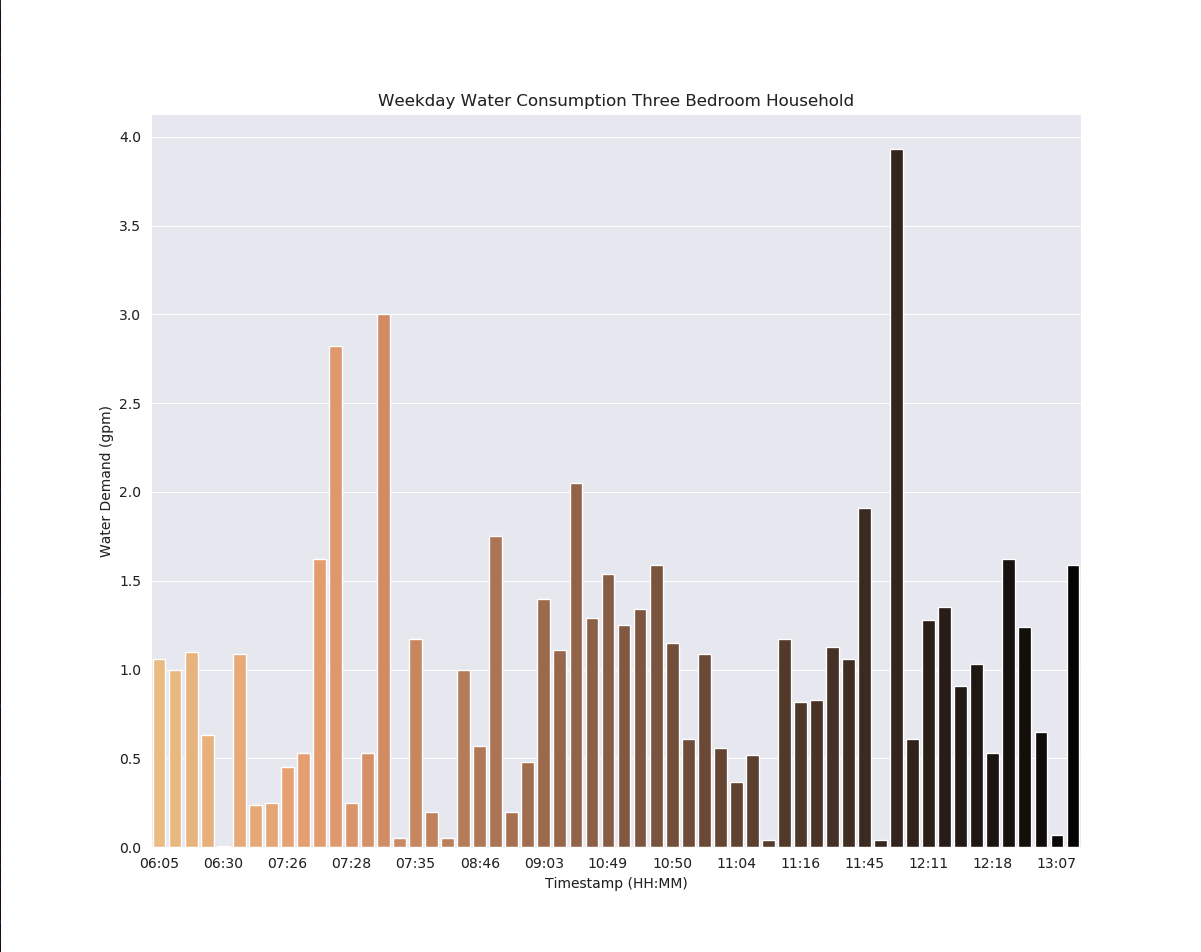
\includegraphics[width=1.1\columnwidth]{Pictures/water_demand_sample.png}
    \caption{Water Demand Sample}
    %\label{fig:temp_data}
\end{figure}

\newpage

\begin{figure}[H]
    \centering
    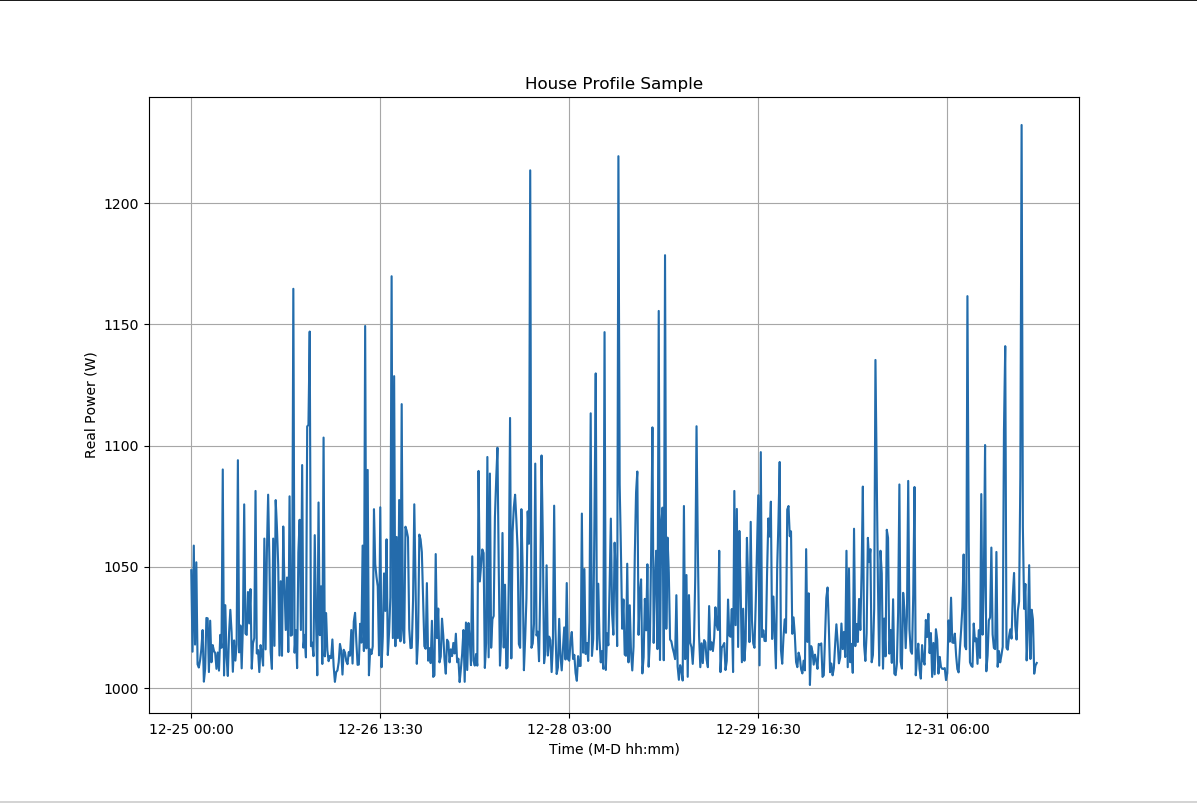
\includegraphics[width=1.1\columnwidth]{Pictures/house_profile_sample.png}
    \caption{ }
    %\label{fig:temp_data}
\end{figure}

\newpage

// ==================================================================================

\begin{figure}[H]
    \centering
    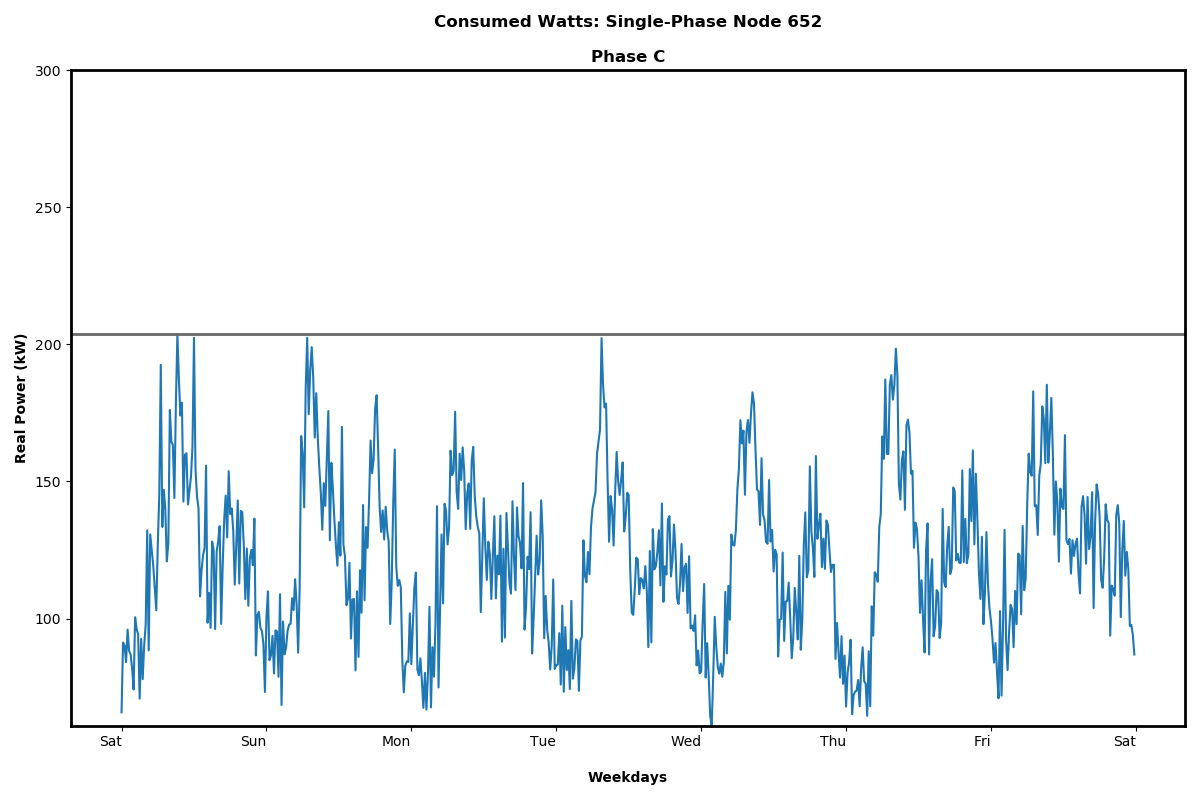
\includegraphics[width=1.1\columnwidth]{Pictures/basecase_single_phase_652_power.png}
    \caption{ }
    %\label{fig:basecase_pow}
\end{figure}

\newpage

\begin{figure}[H]
    \centering
    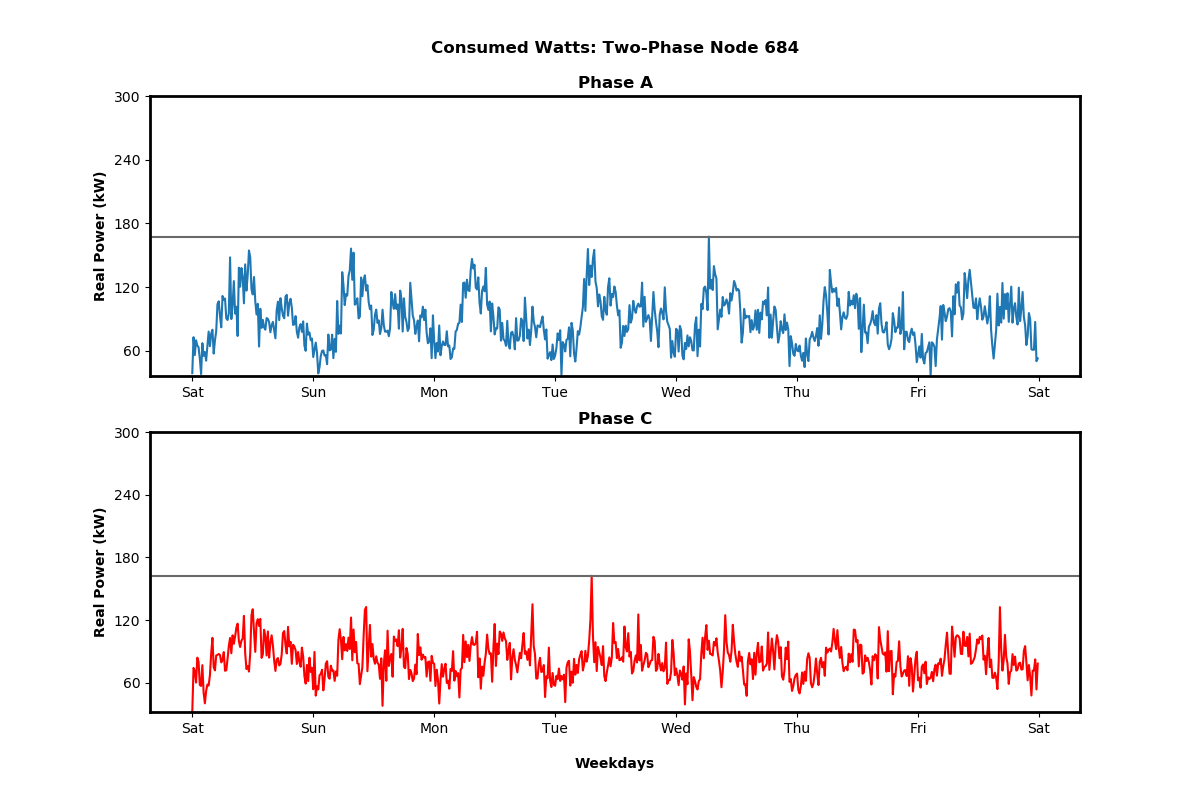
\includegraphics[width=1.1\columnwidth]{Pictures/basecase_two_phase_684_power.png}
    \caption{ }
    %\label{fig:temp_data}
\end{figure}

\newpage

\begin{figure}[H]
    \centering
    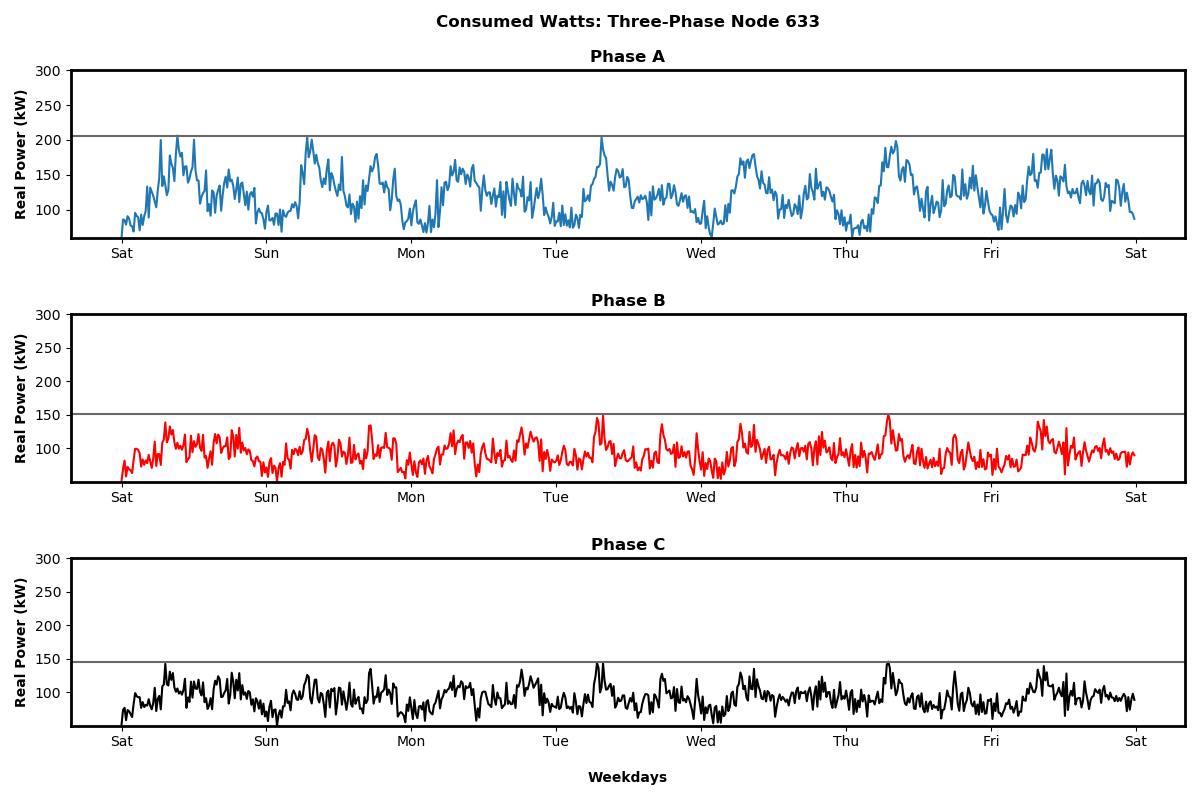
\includegraphics[width=1.1\columnwidth]{Pictures/basecase_three_phase_633_power.png}
    \caption{ }
    %\label{fig:temp_data}
\end{figure}
\newpage


\begin{figure}[H]
    \centering
    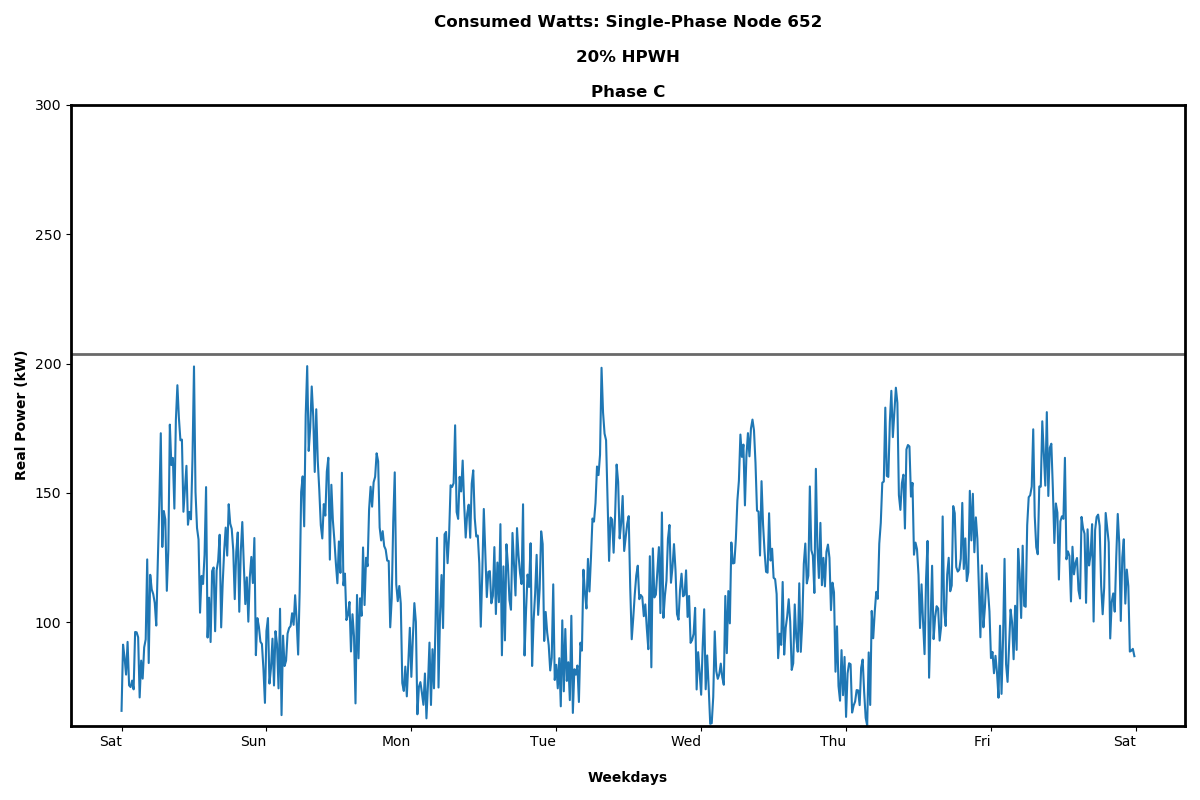
\includegraphics[width=1.1\columnwidth]{Pictures/twenty_single_phase_652_power.png}
    \caption{ }
    %\label{fig:basecase_pow}
\end{figure}

\newpage

\begin{figure}[H]
    \centering
    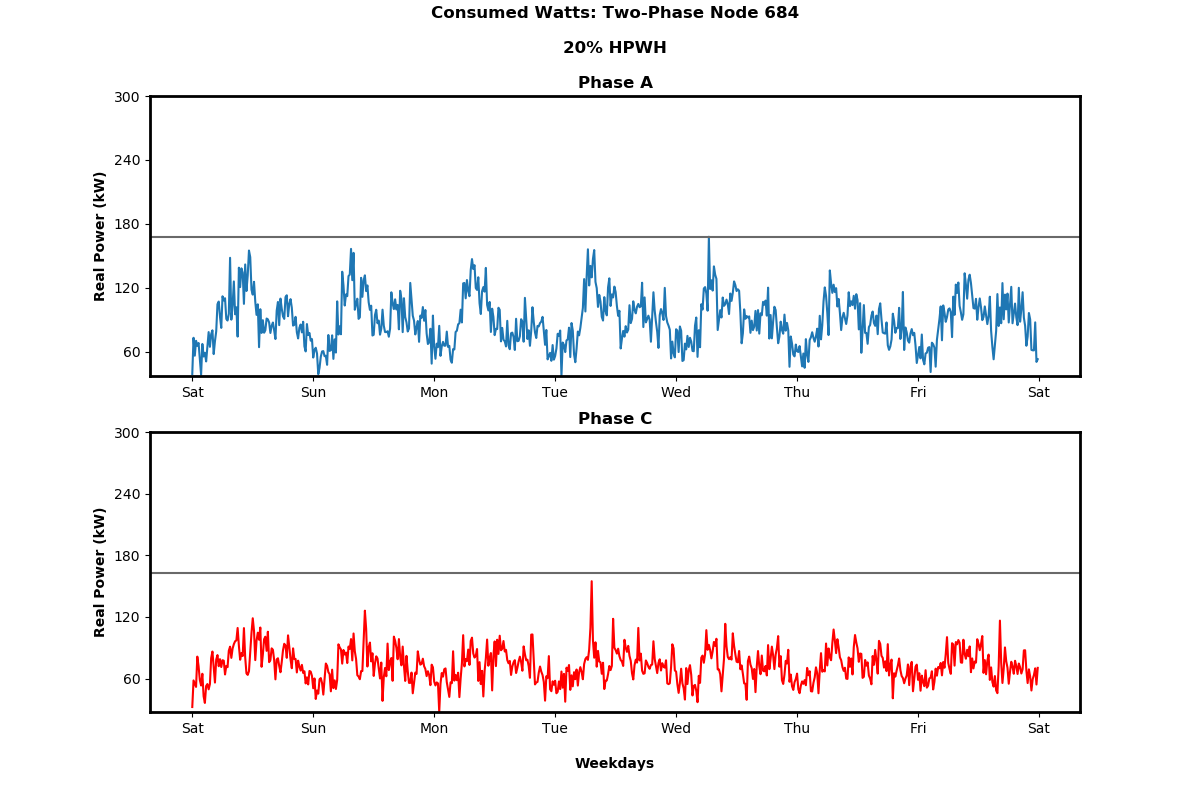
\includegraphics[width=1.1\columnwidth]{Pictures/twenty_two_phase_684_power.png}
    \caption{ }
    %\label{fig:temp_data}
\end{figure}

\newpage

\begin{figure}[H]
    \centering
    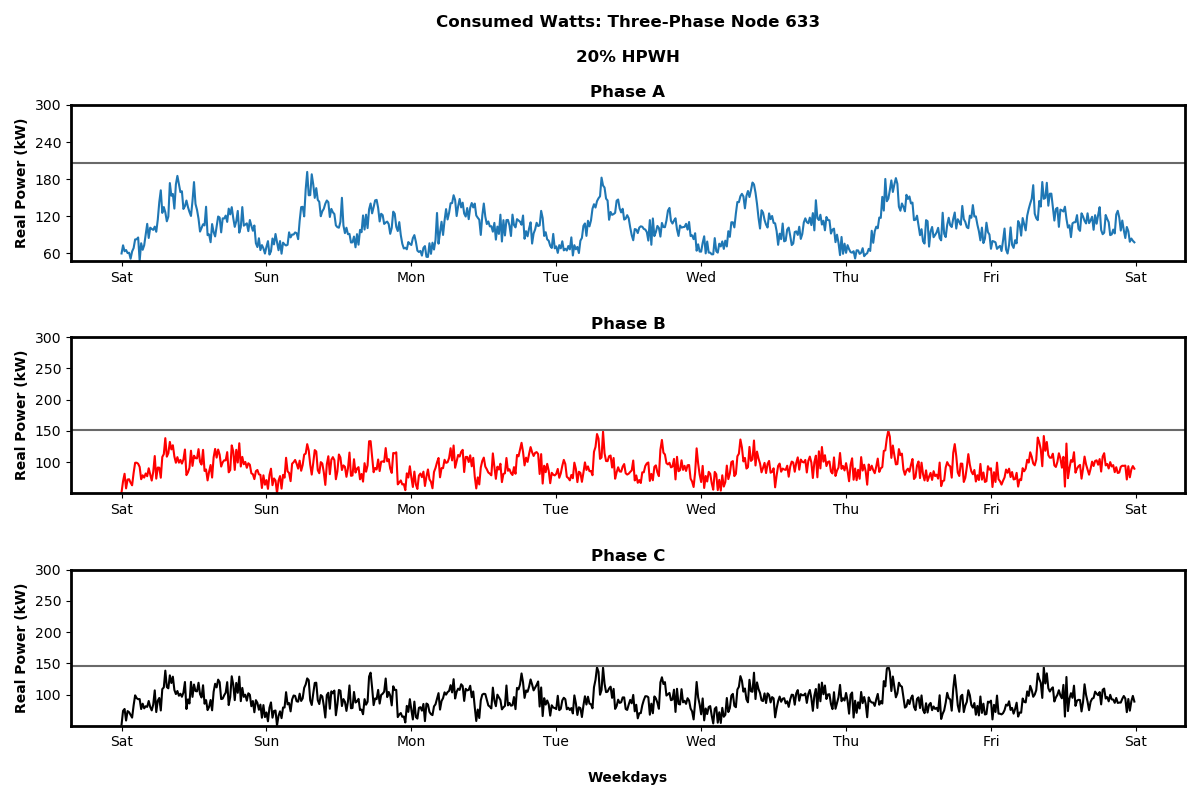
\includegraphics[width=1.1\columnwidth]{Pictures/twenty_three_phase_633_power.png}
    \caption{ }
    %\label{fig:temp_data}
\end{figure}




\begin{figure}[H]
    \centering
    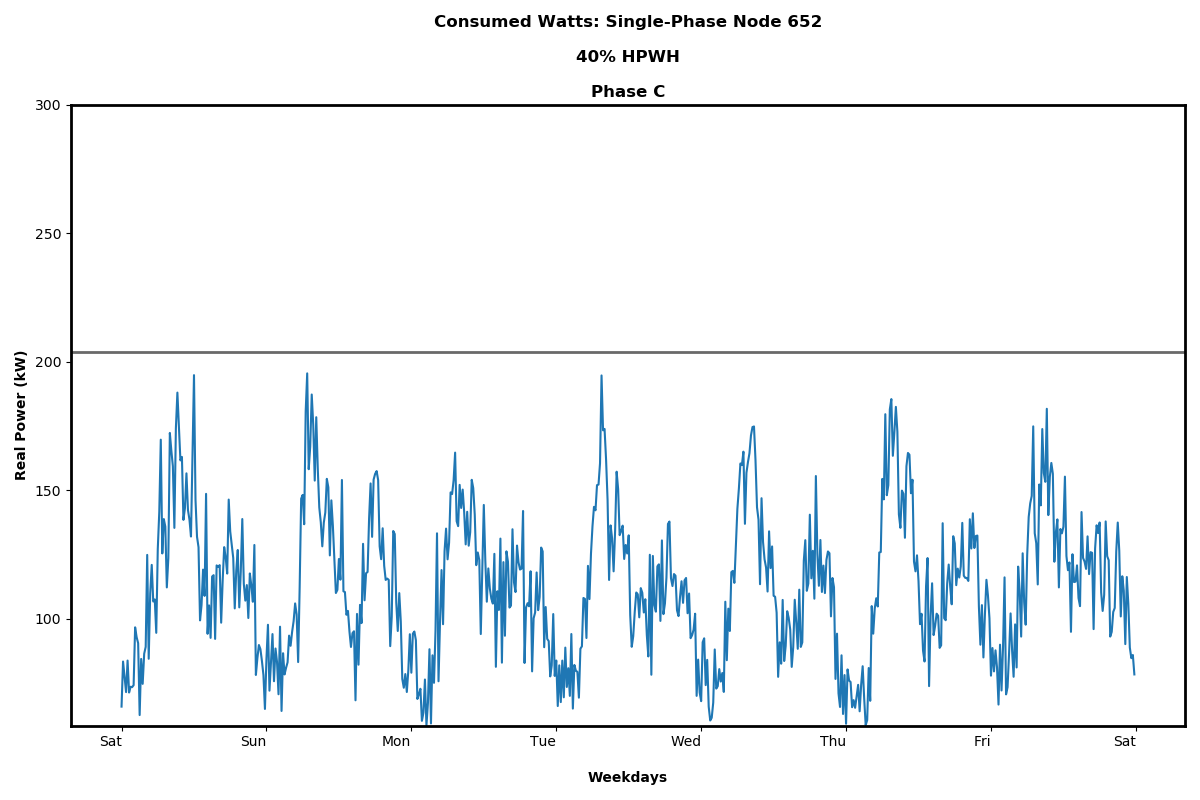
\includegraphics[width=1.1\columnwidth]{Pictures/fourty_single_phase_652_power.png}
    \caption{ }
    %\label{fig:basecase_pow}
\end{figure}

\newpage

\begin{figure}[H]
    \centering
    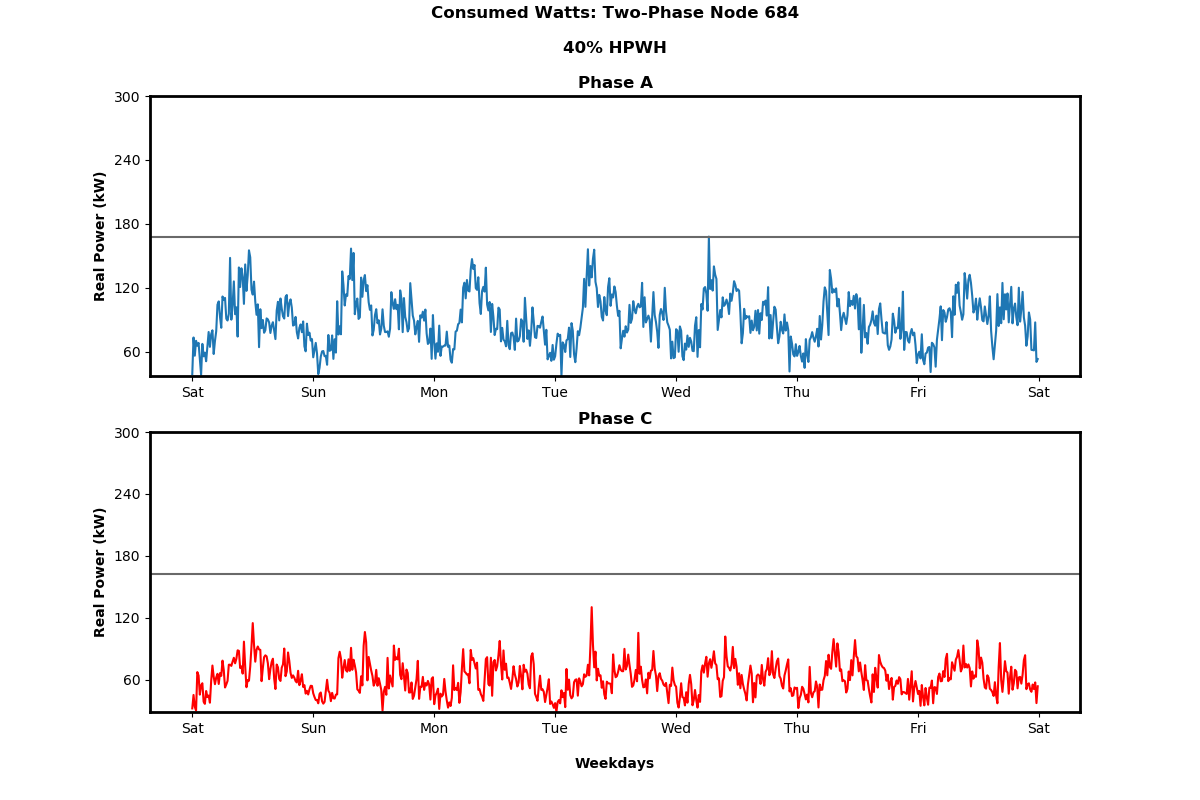
\includegraphics[width=1.1\columnwidth]{Pictures/fourty_two_phase_684_power.png}
    \caption{ }
    %\label{fig:temp_data}
\end{figure}

\newpage

\begin{figure}[H]
    \centering
    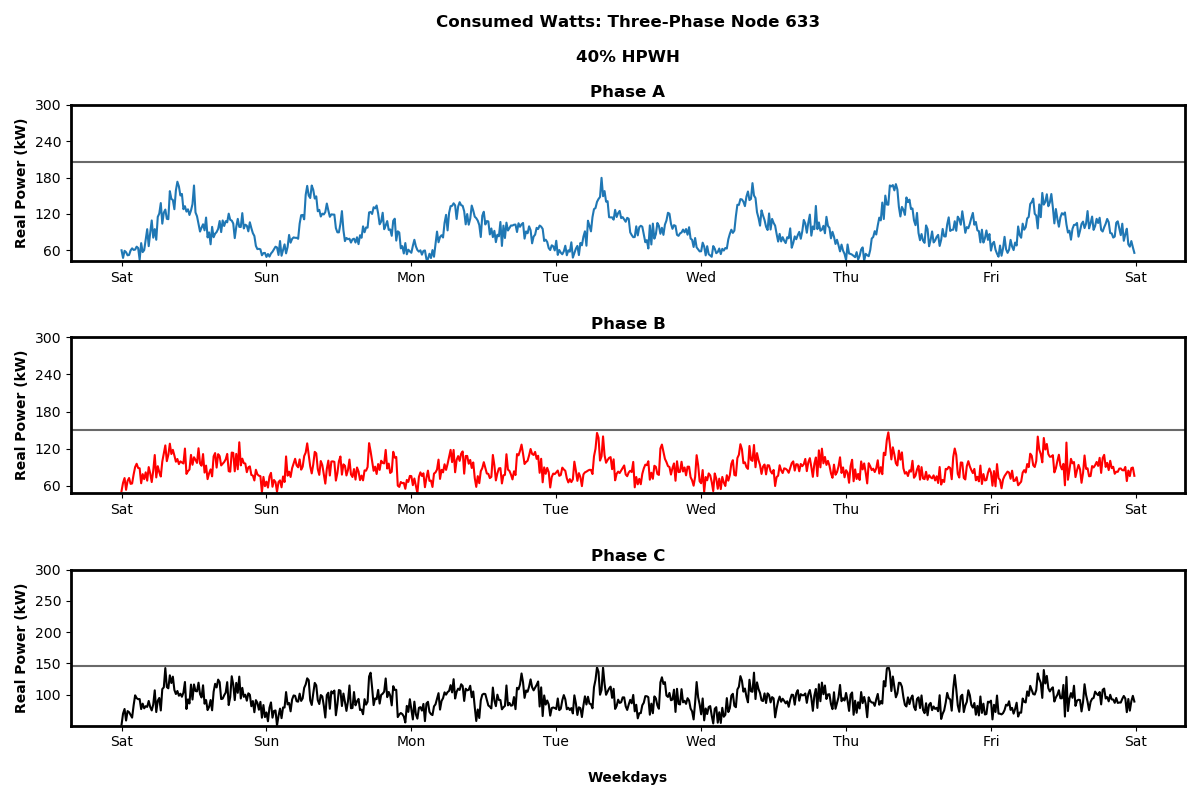
\includegraphics[width=1.1\columnwidth]{Pictures/fourty_three_phase_633_power.png}
    \caption{ }
    %\label{fig:temp_data}
\end{figure}

\newpage



\begin{figure}[H]
    \centering
    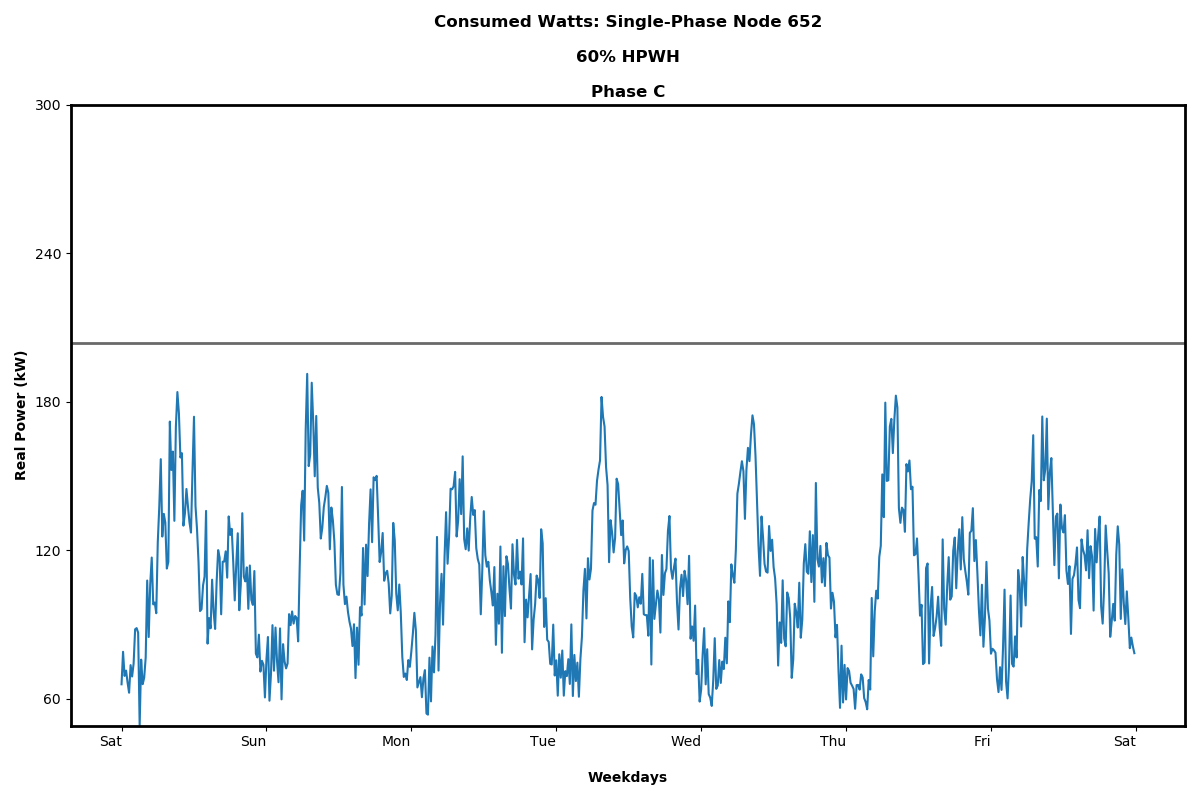
\includegraphics[width=1.1\columnwidth]{Pictures/sixty_single_phase_652_power.png}
    \caption{ }
    %\label{fig:basecase_pow}
\end{figure}

\newpage

\begin{figure}[H]
    \centering
    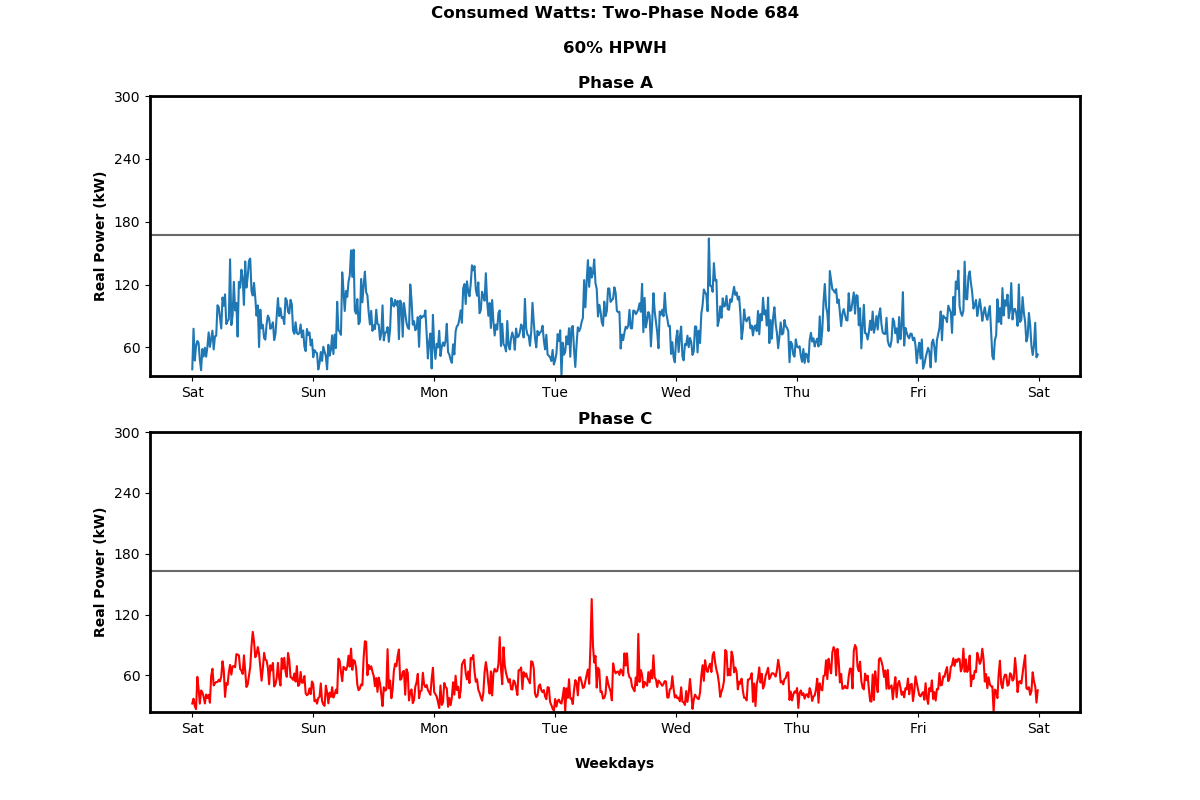
\includegraphics[width=1.1\columnwidth]{Pictures/sixty_two_phase_684_power.png}
    \caption{ }
    %\label{fig:temp_data}
\end{figure}

\newpage

\begin{figure}[H]
    \centering
    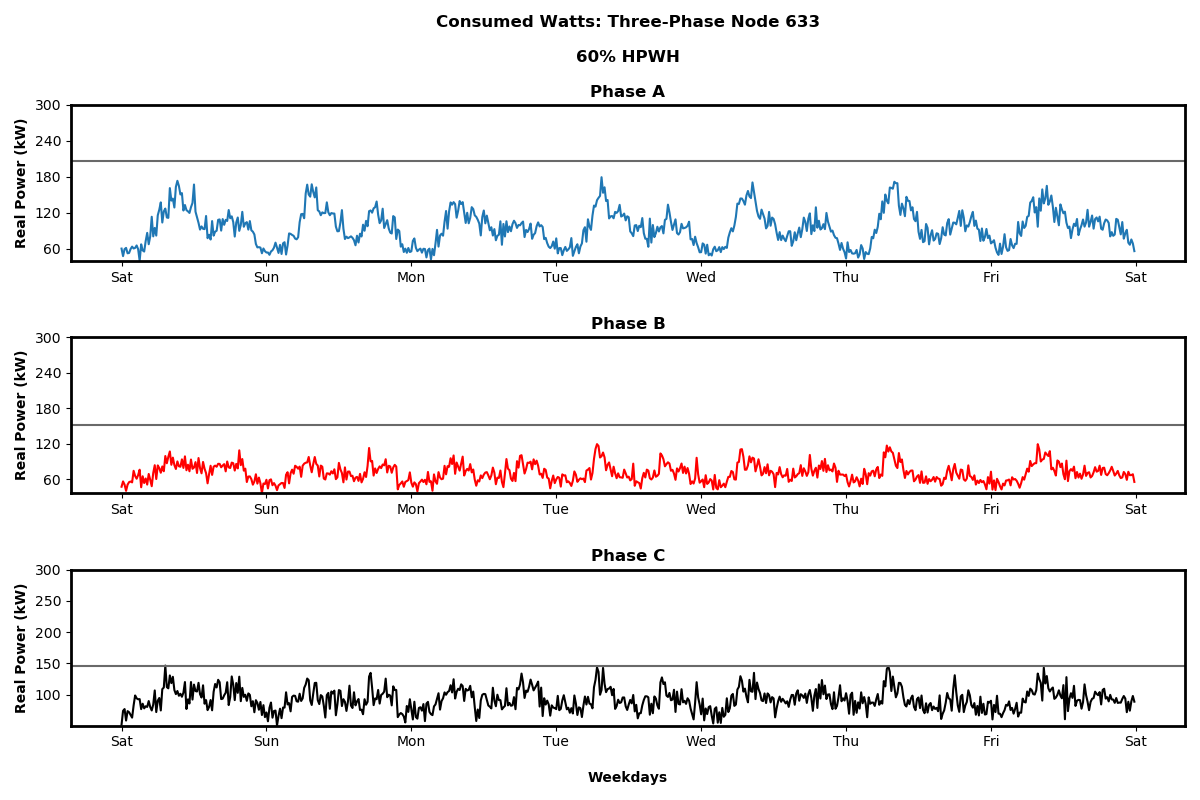
\includegraphics[width=1.1\columnwidth]{Pictures/sixty_three_phase_633_power.png}
    \caption{ }
    %\label{fig:temp_data}
\end{figure}
\newpage





\begin{figure}[H]
    \centering
    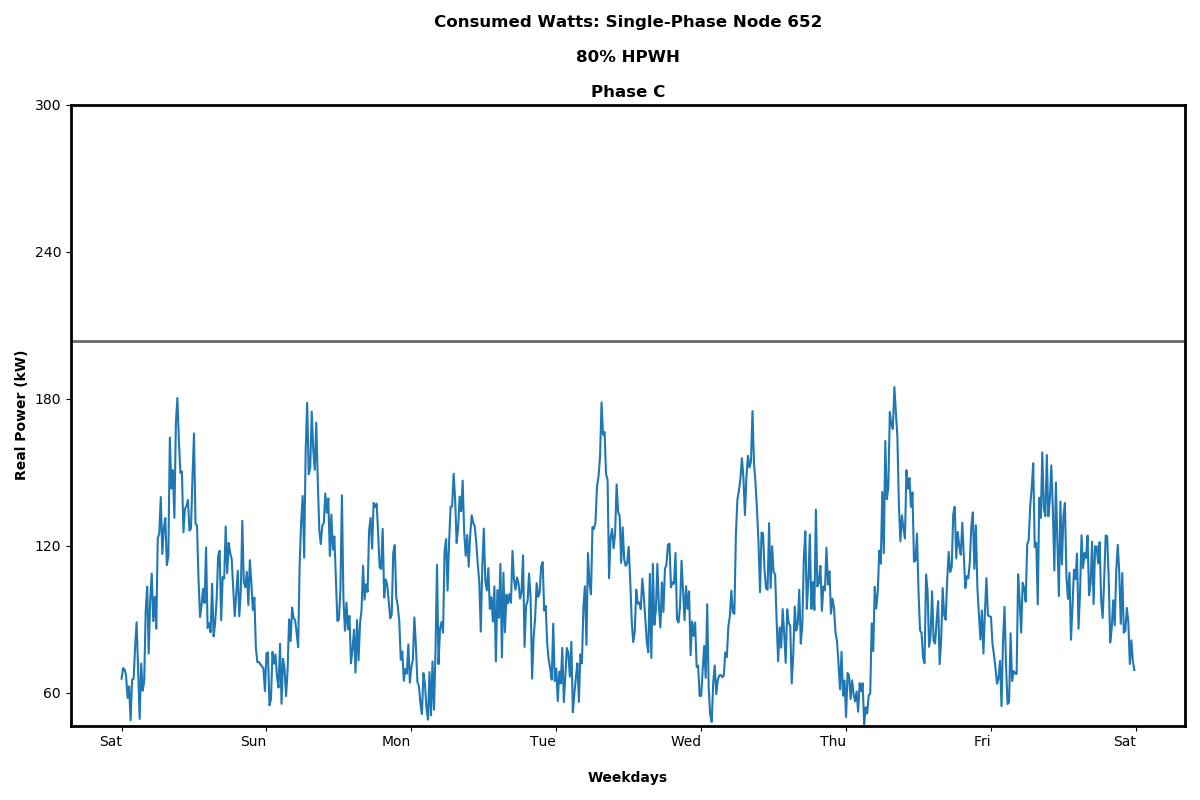
\includegraphics[width=1.1\columnwidth]{Pictures/eighty_single_phase_652_power.png}
    \caption{ }
    %\label{fig:basecase_pow}
\end{figure}

\newpage

\begin{figure}[H]
    \centering
    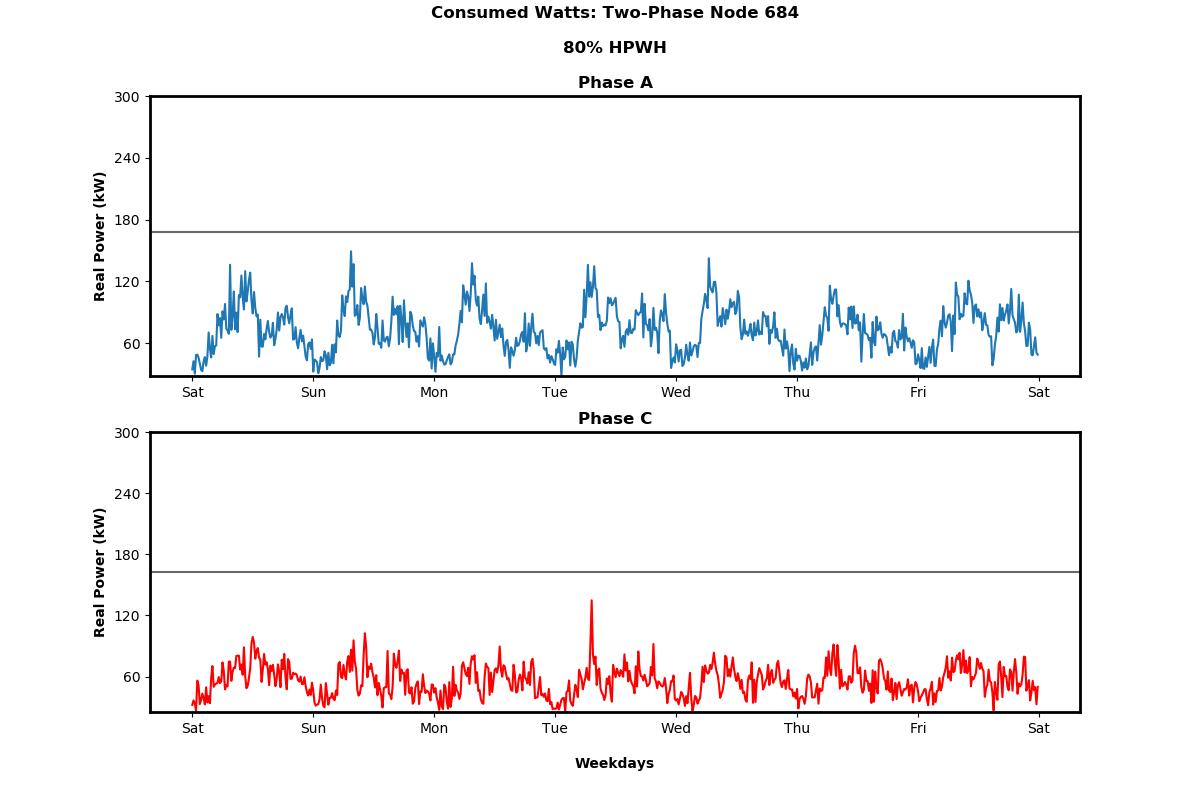
\includegraphics[width=1.1\columnwidth]{Pictures/eighty_two_phase_684_power.png}
    \caption{ }
    %\label{fig:temp_data}
\end{figure}

\newpage

\begin{figure}[H]
    \centering
    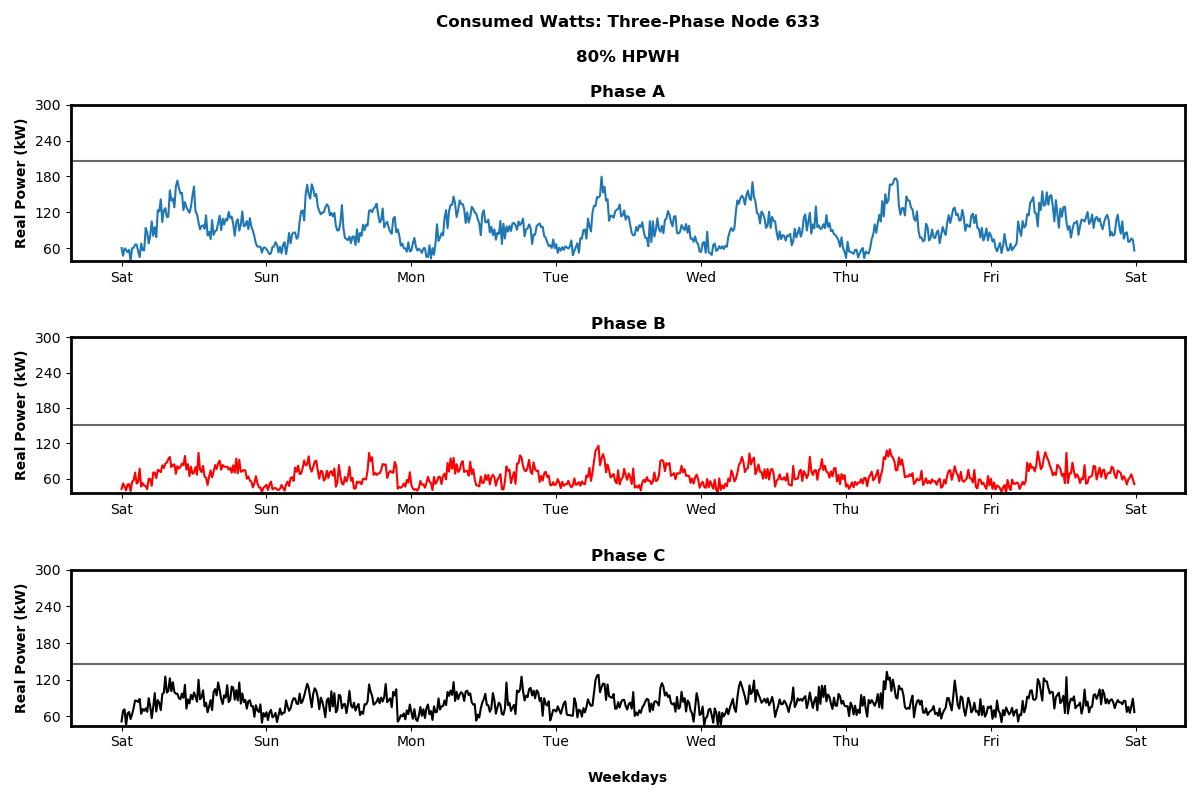
\includegraphics[width=1.1\columnwidth]{Pictures/eighty_three_phase_633_power.png}
    \caption{ }
    %\label{fig:temp_data}
\end{figure}

\newpage





\begin{figure}[H]
    \centering
    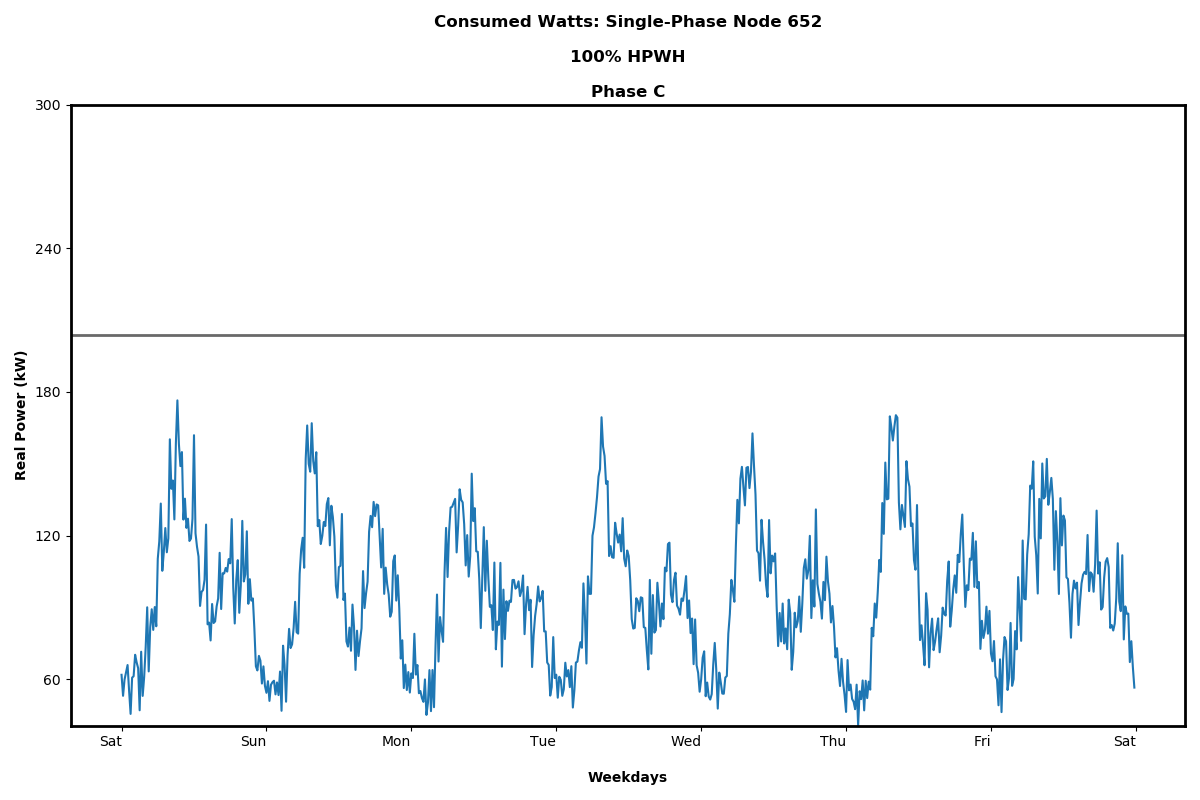
\includegraphics[width=1.1\columnwidth]{Pictures/hundred_single_phase_652_power.png}
    \caption{ }
    %\label{fig:basecase_pow}
\end{figure}

\newpage

\begin{figure}[H]
    \centering
    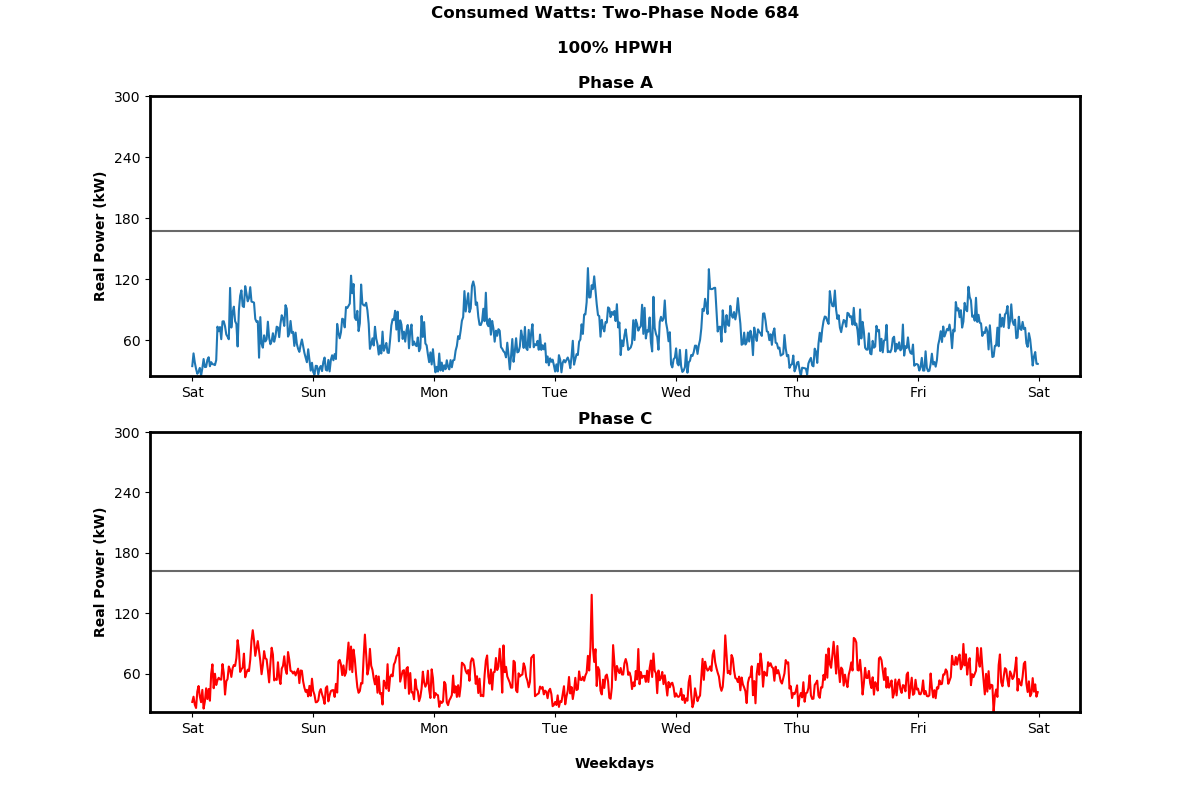
\includegraphics[width=1.1\columnwidth]{Pictures/hundred_two_phase_684_power.png}
    \caption{ }
    %\label{fig:temp_data}
\end{figure}

\newpage

\begin{figure}[H]
    \centering
    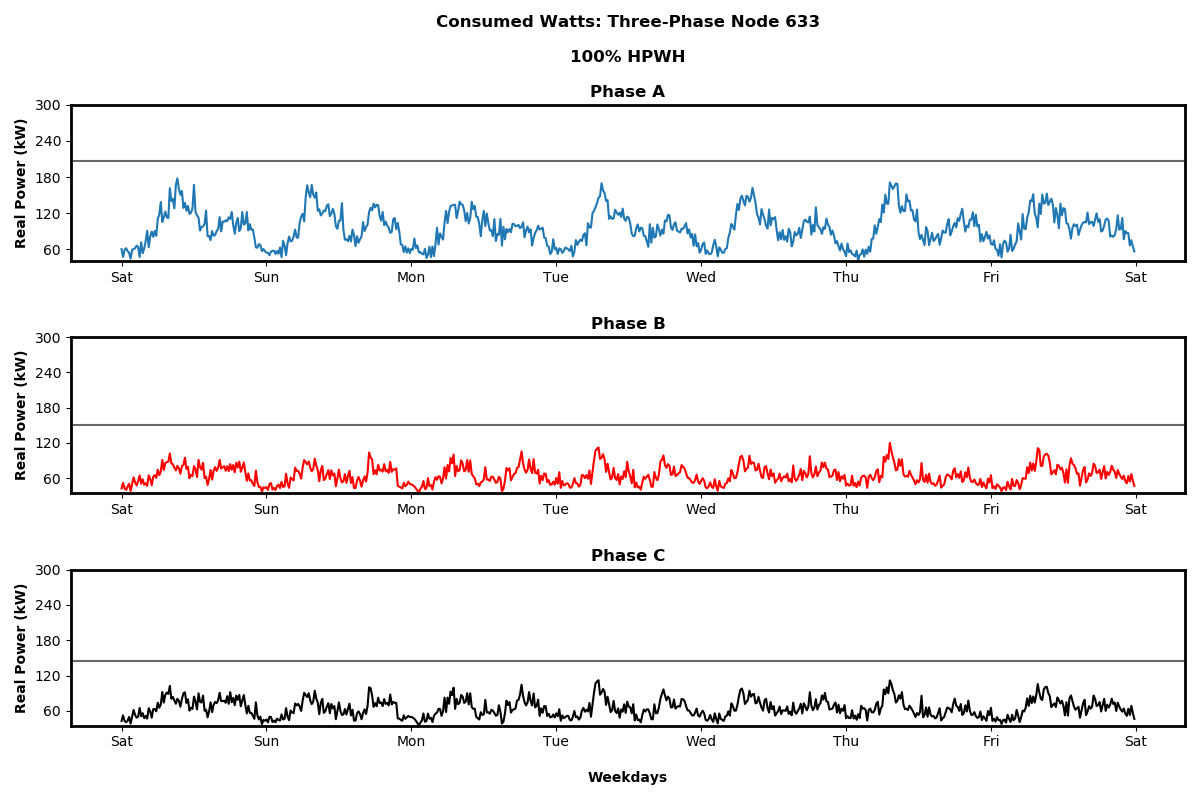
\includegraphics[width=1.1\columnwidth]{Pictures/hundred_three_phase_633_power.png}
    \caption{ }
    %\label{fig:temp_data}
\end{figure}



// ==================================================================================

\begin{figure}[H]
    \centering
    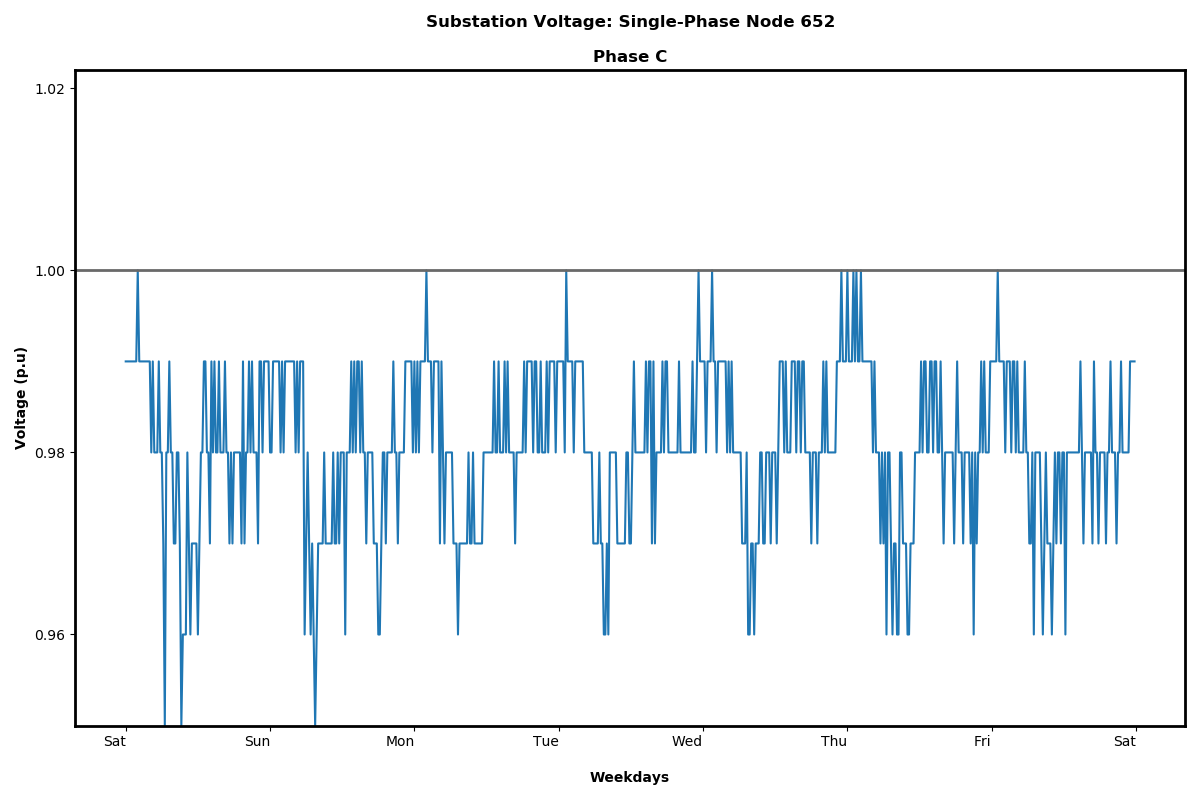
\includegraphics[width=1.1\columnwidth]{Pictures/basecase_single_phase_652_volt.png}
    \caption{ }
    %\label{fig:basecase_pow}
\end{figure}

\newpage

\begin{figure}[H]
    \centering
    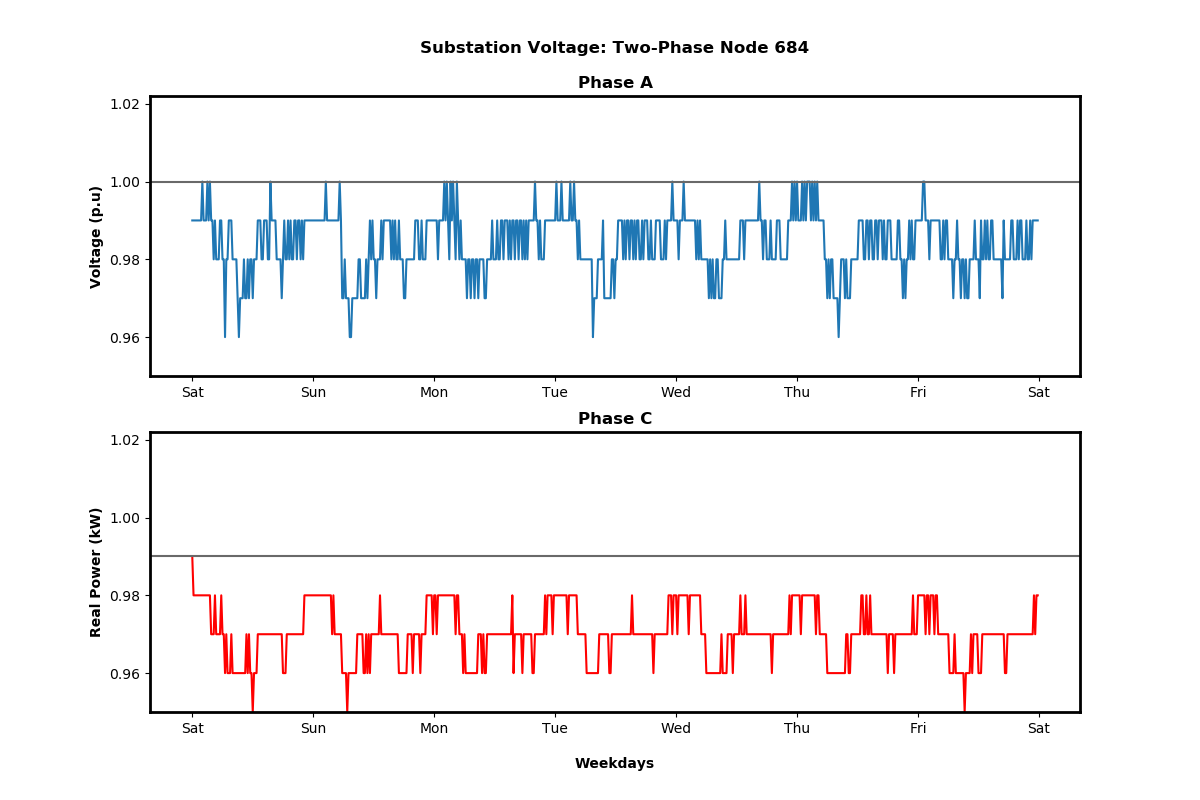
\includegraphics[width=1.1\columnwidth]{Pictures/basecase_two_phase_684_volt.png}
    \caption{ }
    %\label{fig:temp_data}
\end{figure}

\newpage

\begin{figure}[H]
    \centering
    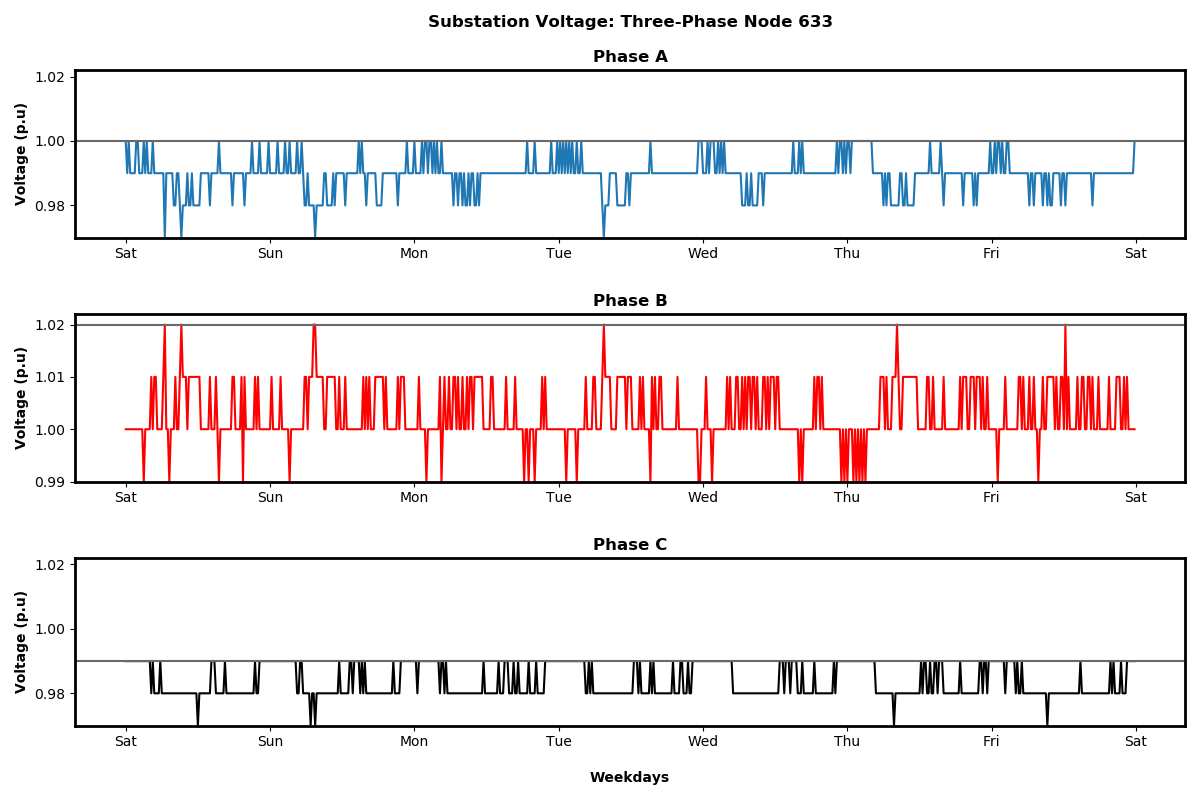
\includegraphics[width=1.1\columnwidth]{Pictures/basecase_three_phase_633_volt.png}
    \caption{ }
    %\label{fig:temp_data}
\end{figure}
\newpage


\begin{figure}[H]
    \centering
    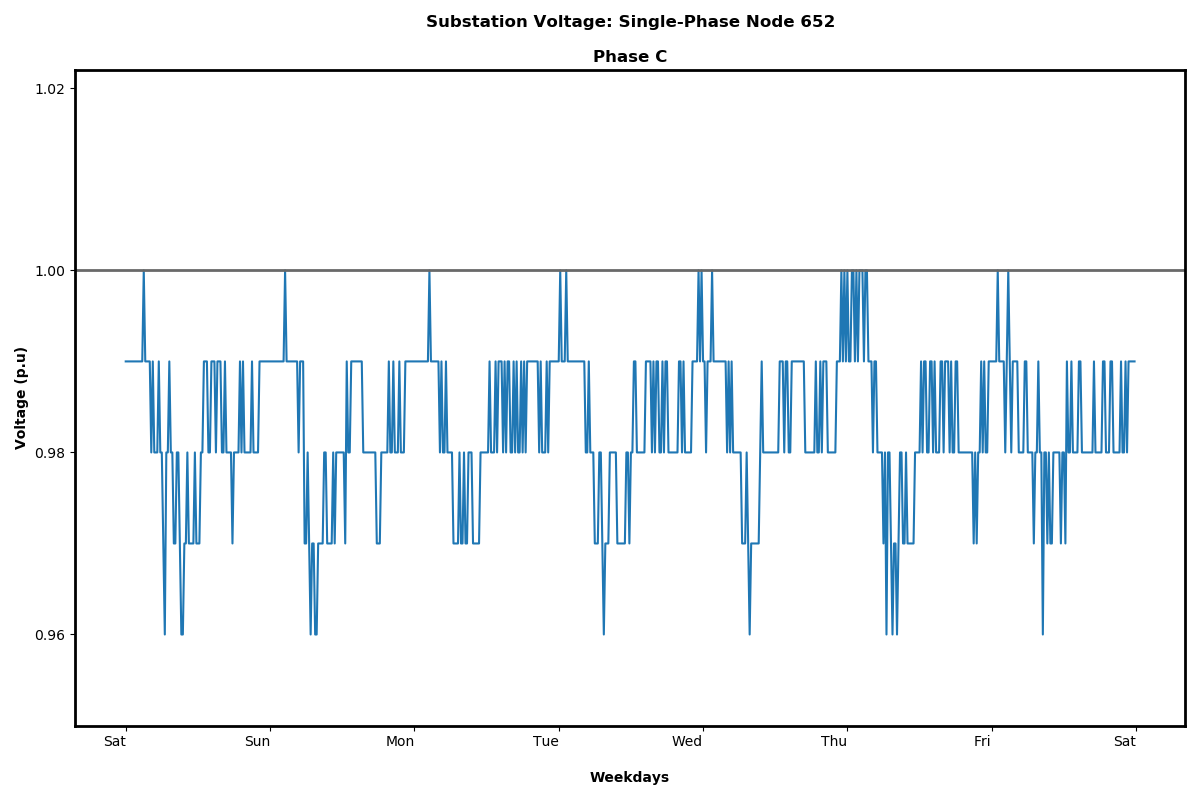
\includegraphics[width=1.1\columnwidth]{Pictures/twenty_single_phase_652_volt.png}
    \caption{ }
    %\label{fig:basecase_pow}
\end{figure}

\newpage

\begin{figure}[H]
    \centering
    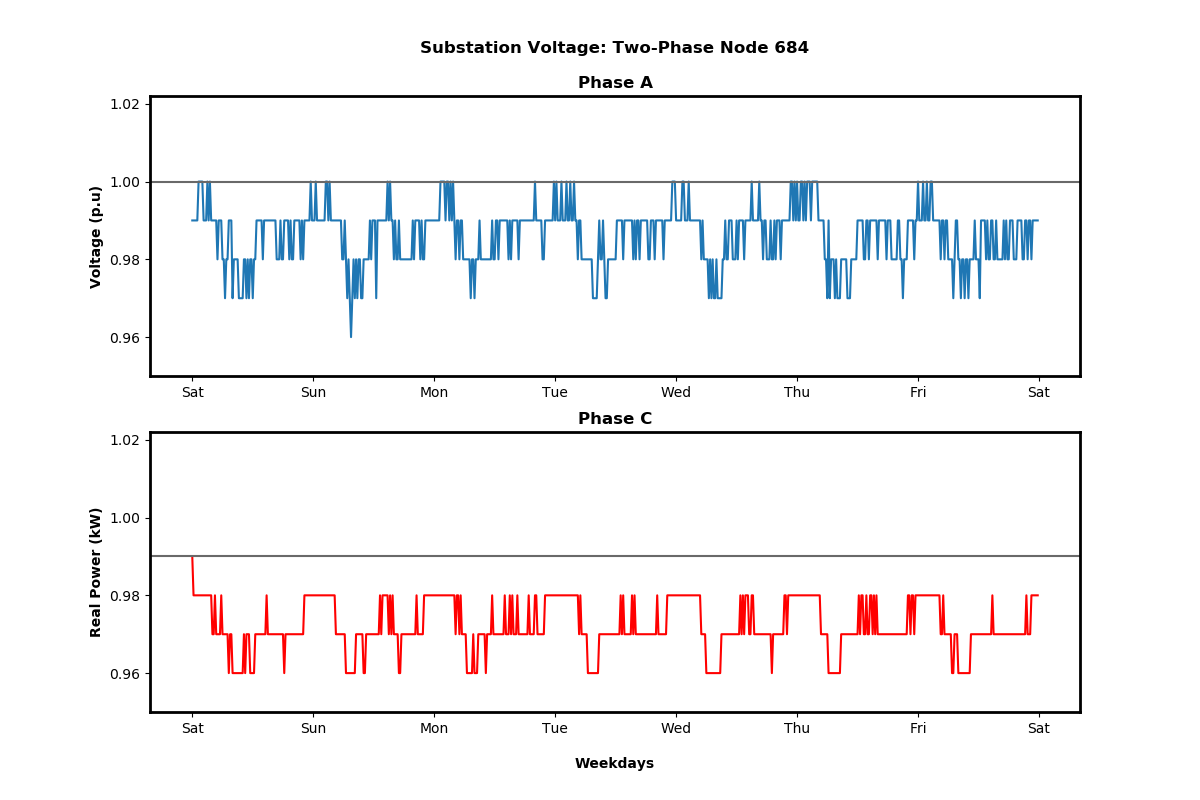
\includegraphics[width=1.1\columnwidth]{Pictures/twenty_two_phase_684_volt.png}
    \caption{ }
    %\label{fig:temp_data}
\end{figure}

\newpage

\begin{figure}[H]
    \centering
    \includegraphics[width=1.1\columnwidth]{Pictures/twenty_three_phase_633_volt.png}
    \caption{ }
    %\label{fig:temp_data}
\end{figure}




\begin{figure}[H]
    \centering
    \includegraphics[width=1.1\columnwidth]{Pictures/fourty_single_phase_652_volt.png}
    \caption{ }
    %\label{fig:basecase_pow}
\end{figure}

\newpage

\begin{figure}[H]
    \centering
    \includegraphics[width=1.1\columnwidth]{Pictures/fourty_two_phase_684_volt.png}
    \caption{ }
    %\label{fig:temp_data}
\end{figure}

\newpage

\begin{figure}[H]
    \centering
    \includegraphics[width=1.1\columnwidth]{Pictures/fourty_three_phase_633_volt.png}
    \caption{ }
    %\label{fig:temp_data}
\end{figure}

\newpage



\begin{figure}[H]
    \centering
    \includegraphics[width=1.1\columnwidth]{Pictures/sixty_single_phase_652_volt.png}
    \caption{ }
    %\label{fig:basecase_pow}
\end{figure}

\newpage

\begin{figure}[H]
    \centering
    \includegraphics[width=1.1\columnwidth]{Pictures/sixty_two_phase_684_volt.png}
    \caption{ }
    %\label{fig:temp_data}
\end{figure}

\newpage

\begin{figure}[H]
    \centering
    \includegraphics[width=1.1\columnwidth]{Pictures/sixty_three_phase_633_volt.png}
    \caption{ }
    %\label{fig:temp_data}
\end{figure}
\newpage





\begin{figure}[H]
    \centering
    \includegraphics[width=1.1\columnwidth]{Pictures/eighty_single_phase_652_volt.png}
    \caption{ }
    %\label{fig:basecase_pow}
\end{figure}

\newpage

\begin{figure}[H]
    \centering
    \includegraphics[width=1.1\columnwidth]{Pictures/eighty_two_phase_684_volt.png}
    \caption{ }
    %\label{fig:temp_data}
\end{figure}

\newpage

\begin{figure}[H]
    \centering
    \includegraphics[width=1.1\columnwidth]{Pictures/eighty_three_phase_633_volt.png}
    \caption{ }
    %\label{fig:temp_data}
\end{figure}

\newpage





\begin{figure}[H]
    \centering
    \includegraphics[width=1.1\columnwidth]{Pictures/hundred_single_phase_652_volt.png}
    \caption{}
    %\label{fig:basecase_pow}
\end{figure}

\newpage

\begin{figure}[H]
    \centering
    \includegraphics[width=1.1\columnwidth]{Pictures/hundred_two_phase_684_volt.png}
    \caption{}
    %\label{fig:temp_data}
\end{figure}

\newpage

\begin{figure}[H]
    \centering
    \includegraphics[width=1.1\columnwidth]{Pictures/hundred_three_phase_633_volt.png}
    \caption{}
    %\label{fig:temp_data}
\end{figure}

\newpage

% \section{GridAPPS-D}

% \subsection{Converting GLM files to CIM Files}

% GridAPPS-D uses cim file format. In our case, we have several glm file models (GridLAB-D) that we want to convert to CIM file format (GridAPPS-D format). This process can be done by using scripts within GridAPPS-D repository. 

% Some issues exist, however, when converting from GLM files to CIM files. These issues lie within the ``house objects'' in GridLAB-D. The conversion scripts will convert each ``house object'' to a ``triplex load''. This might affect the model overall as we use these ``house objects'' to provide weather environment for the \gls{hpwh}. 

% This is not a big deal and I believe we can easily figure a work around that by simply remove the ``house objects''. Keep in mind that the ``house objects'' are linked with other objects. So a model reconfiguration might be needed. The other workaround is to use the IEEE 13 node feeder as it is within GridAPPS-D, then use ``insertDER.py'' script to add the required loads and triplex configurations.

% \subsubsection{Questions}
% \begin{itemize}
% \item In the GLM file, we use several load profiles that are read by the triplex load objects. If we convert the GLM file to a CIM file, can we still use these load profiles?
% \end{itemize}

\pagebreak

\newpage
\section{Summer 2022}
% \label{Summer2022}
This section addresses the work progress within the ME. Refer to Sean Keene's thesis to get how the system is set up. This document, however, addresses an issue that is related to GridAPPS-D flexibility. 

\subsection{Problem Statement}

\begin{figure}[htp!]
    \centering
    \includegraphics[width=0.7\columnwidth]{Pictures/model_conversion.png}
    \caption{GridAPPS-D Model Conversion}
    \label{fig:me_gridappsd}
\end{figure}

As shown in Figure~\ref{fig:me_gridappsd}, GridAPPS-D takes an input file (IEEE Test Feeders, PNNL Taxonomy Feeders, or EPRI Test Circuits) as a \textbf{dss} format. Within each \textbf{dss} file,
''export cim100'' command is used to export an XML version of the \textbf{dss} file. The XML file is then stored in the Triple Store database so it can be adjusted as needed. 


Over the years, the PowerLab team has been extensively working with GridLAB-D. The PowerLab team has developed several \textbf{glm} scripts to implement studies and cases. Many of these studies are slightly or non-GridAPPS-D-related. 
The time has come to merge many of these studies within the Modelling Environment (ME). This Section is meant to walk through the progress of implementing scripts that convert \textbf{glm} files to \textbf{dss}.

\subsection{Objectives}
\begin{itemize}
    \item Convert \textbf{glm} files to \textbf{Common Information Model (CIM)}.
    \item Insert the appropriate loads in the specified \textbf{glm} file using GridAPPS-D.
    \item Develop communication between entities and demand response capabilities.
\end{itemize}

\subsection{Tools to be Used}

\begin{itemize}
    \item To convert from GridLAB-D to OpenDSS, I used \href{https://github.com/NREL/ditto}{Ditto-CLI}
    \item To edit the \textbf{glm} files, I used \href{https://github.com/NREL/glm}{glm} module in Python.
    \item To convert from \textbf{dss} to \textbf{CIM}, I used \href{https://cimhub.readthedocs.io/en/latest/Tutorial.html#ieee-123-bus-base-case}{CIMhub}
\end{itemize}

\subsection{Processing Steps}

\begin{figure}[htp!]
    \centering
    \includegraphics[width=0.7\columnwidth]{Pictures/glm_conversion_tool.png}
    \caption{File Conversion Processing Chart}
    \label{fig:me_conversion}
\end{figure}

\subsubsection{Step 1: Edit \textbf{glm} Files}

GridLAB-D and OpenDSS are different software packages and, therefore, they are not expected to have the same models. To find out which GridLAB-D objects are compatible with OpenDSS models, I went through test files 
within \href{https://github.com/NREL/ditto}{Ditto-CLI}. The \href{run:/home/deras/Desktop/Midrar_work/ditto/tests/data/small_cases/gridlabd/ieee_4node/node.glm}{Node.glm} is a \textbf{glm} file that can be easily 
converted to \textbf{dss} without errors. The content of this file is compared with the \textbf{glm} that I developed to ensure a smooth and accurate transition between GridLAB-D and OpenDSS. These models are as follows:

\begin{itemize}
    \item Clock
    \item module powerflow
    \item overhead line conductor
    \item line spacing
    \item line configuration
    \item transformer configuration
    \item node object
    \item overhead line object
    \item transformer objects
    \item load object
\end{itemize}

Note that objects like triplex load and water heaters are not included. Whether these objects can be implemented or not is not the question. The question is, 
do they align with the final objective of this work? Given that \textbf{CIM} files are general models, and their behavior mimics the operation of the aforementioned loads,
then the answer is no, they are not needed. 

To delete such objects from the GridLAB-D file (or \textbf(glm) file), we need a tool to access the \textbf(glm) file and perform the required edits. This editor as far as 
the author's knowledge does not exist. Therefore, I used the \href{https://github.com/NREL/glm}{GLM} module in Python. module in python. This module converts \textbf(glm) files to JSON and vice-versa. It's easy to deal with 
JSON files with python. Once the \textbf(glm) file is converted to JSON, the following objects were deleted:
\begin{itemize}
    \item triplex\_load objects.
    \item triplex\_line objects.
    \item house objects.
    \item waterheater objects.
    \item multi\_recoreder objects.
    \item player objects.
    \item capacitor objects.
\end{itemize}

Again, as far as the author's knowledge, these objects do not have similar models in OpenDSS. The next step is to convert the JSON file back to a \textbf(glm) format. There are 
several crucial factors to note here:

\begin{itemize}
    \item During the conversion process, the \textit(clock) object has double quotes instead of single quotes. GridLAB-D compiler does not interpret the double quotes correctly, so they need to 
    be changed to single quotes.
    \item The 13-node feeder contains 13 nodes. However, only 10 nodes are used due to reasons mentioned in \href{https://pdxscholar.library.pdx.edu/open_access_etds/6101/}{Midrar's Thesis}.
    Some branch nodes are not used within the 13-node feeder and these are as follows:
    \begin{itemize}
        \item Node 6711
        \item Node 6321
        \item Node 634
        \item Node 650
        \item Node 630
    \end{itemize}
\end{itemize}
To ensure an accurate and smooth conversion from GridLAB-D to OpenDSS, run the \textbf(glm) file and the \textbf(dss) file and make sure they run correctly without errors and have the same
results.

\subsubsection{Ditto-CLI}
To convert a \textbf{glm} file to \textbf{dss}, the following command may be used:
\begin{lstlisting}[language=bash]
    $ ditto-cli convert --input ``glm file name'' --from gridlabd --to opendss --output ``output file directory''
\end{lstlisting}

The \href{https://github.com/NREL/ditto}{Ditto-CLI} tool does most of the work for those who want to convert GridLAB-D files to OpenDSS and vice-versa. However, it is not perfect and it has its 
shortfalls. several errors in particular that have been showing most of the time are the following:
\begin{lstlisting}[language=python]
    $ Matrix Inversion Error for Line ``line name''.
    $ TLineObj.CalcYPrim.
    $ Access violation.
\end{lstlisting}
Such errors are caused by the length and impedance conversions of the overhead and underground lines. In my case, since I'm working on the 13-node feeder, I need to make sure the original length
parameters and impedance matrices are the same as the one I have. After the conversion, run the \textbf{dss} file and if it outputs similar errors as above, do the following:
\begin{itemize}
    \item edit ``LineCodes.dss'' file.
    \item change the ``R'' and ``X'' matrices and ensure they correspond to the original IEEE-13 Node Feeder.
    \item All original IEEE feeders in \textbf{dss} format can be found in \href{https://github.com/tshort/OpenDSS/tree/master/Distrib/IEEETestCases}{DSS Github Repository}
\end{itemize}

\subsection{Important opendsscmd Commands}
\begin{itemize}
    \item To export an XML version of the current \textbf{dss} feeder, insert the following command within the ``Master.dss'' file:
    \begin{lstlisting}[language=python]
        $ export cim100
    \end{lstlisting}
    \item To export a CIM version of the current \textbf{dss} file, create a script containing the following and name it ``export\_cim.dss'':
    \begin{lstlisting}[language=python]
        redirect Master.dss
        solve
        export y triplet base_ysparse.csv
        export ynodelist base_nodelist.csv
        export summary base_summary.csv
    \end{lstlisting}
    \item Using opendsscmd command in the terminal, run the above script.
    \item \href{https://sourceforge.net/projects/electricdss/files/OpenDSSCmd/}{Source of the above info}.
\end{itemize}

\pagebreak

%----------------------------------------------------------------------------------------
%	BIBLIOGRAPHY
%----------------------------------------------------------------------------------------
\newpage
\bibliographystyle{unsrt}%Used BibTeX style is unsrt
\bibliography{bibfile}


%----------------------------------------------------------------------------------------
%----------------------------------------------------------------------------------------
%    Section: Authors, Lab, Disclaimer & Acknowledgements
%----------------------------------------------------------------------------------------
\newpage
\input{Bios}
\pagebreak
%----------------------------------------------------------------------------------------

\end{document}
